% StepCharge AI Preliminary Project Report — Academic Year 2026–27
% Department of Information Technology, MVP'S KBTCOE Nashik
% Savitribai Phule Pune University, Pune

\documentclass[12pt,a4paper,oneside]{report}

\usepackage[a4paper,left=1.25in,right=1in,top=1in,bottom=1in]{geometry}
\usepackage{indentfirst}
\usepackage{amsmath,amssymb}
\usepackage{graphicx}
\usepackage{float}
\usepackage{array,booktabs,longtable,tabularx,multirow}
\usepackage{enumitem}
\usepackage{setspace}
\usepackage{titlesec}
\usepackage{fancyhdr}
\usepackage{caption}
\usepackage{subcaption}
\usepackage{tikz}
\usetikzlibrary{arrows.meta,positioning,shapes.geometric,shapes.misc,fit,calc}
\usepackage{hyperref}
\usepackage{xcolor}
\definecolor{amber}{RGB}{255, 191, 0}
\usepackage{url}
\usepackage{tocloft}
\usepackage{listings}

% Hyperref configuration
\hypersetup{
    colorlinks=true,
    linkcolor=black,
    citecolor=black,
    urlcolor=blue!70!black,
    pdftitle={StepCharge AI Preliminary Project Report},
    pdfauthor={[STUDENT NAME 1], [STUDENT NAME 2], [STUDENT NAME 3], [STUDENT NAME 4]}
}

% Spacing & Indentation
\setstretch{1.25}
\setlength{\headheight}{15pt}
\setlength{\parindent}{0.3in}
\setlength{\parskip}{4pt}
\setlist[itemize]{leftmargin=0.35in,itemsep=2pt,topsep=3pt}
\setlist[enumerate]{leftmargin=0.4in,itemsep=3pt,topsep=3pt}

% Chapter & Section Heading Formats
\titleformat{\chapter}[display]{\bfseries\centering\Large}{\chaptername\ \thechapter}{8pt}{\Large}
\titlespacing*{\chapter}{0pt}{-10pt}{14pt}
\titleformat{\section}{\bfseries\large}{\thesection}{0.7em}{}
\titleformat{\subsection}{\bfseries\normalsize}{\thesubsection}{0.7em}{}

% Running Headers & Footers
\pagestyle{fancy}
\fancyhf{}
\fancyhead[L]{\small\nouppercase{StepCharge AI: Smart Footstep Energy Harvesting and Monitoring System}}
\fancyfoot[C]{\thepage}
\renewcommand{\headrulewidth}{0.4pt}
\renewcommand{\footrulewidth}{0pt}

% Captions & Code Listings
\captionsetup{font=small,labelfont=bf}

\lstset{
    basicstyle=\ttfamily\scriptsize,
    keywordstyle=\color{blue!80!black}\bfseries,
    stringstyle=\color{teal!80!black},
    commentstyle=\color{gray!80}\itshape,
    numbers=left,
    numberstyle=\tiny\color{gray},
    stepnumber=1,
    numbersep=6pt,
    backgroundcolor=\color{gray!5},
    frame=single,
    rulecolor=\color{black!20},
    breaklines=true,
    breakatwhitespace=true,
    tabsize=2,
    showstringspaces=false
}

% Project metadata macros
\newcommand{\projecttitle}{StepCharge AI: Smart Footstep Energy Harvesting and Monitoring System}
\newcommand{\college}{MVP'S Karmaveer Baburao Ganpatrao Thakare College of Engineering, Nashik}
\newcommand{\guide}{[GUIDE NAME]}
\newcommand{\coordinator}{[COORDINATOR NAME]}
\newcommand{\hod}{Dr. S. A. Talekar}
\newcommand{\principal}{Dr. S. R. Devane}

\begin{document}

% -------------------- FRONT MATTER --------------------
\pagenumbering{roman}

\begin{titlepage}
\centering
\vspace*{0.10in}

{\Large\bfseries A PRELIMINARY PROJECT REPORT\par}
\vspace{0.08in}

{\large on\par}
\vspace{0.10in}

{\LARGE\bfseries \projecttitle\par}
\vspace{0.14in}

Submitted to Savitribai Phule Pune University, Pune, in partial
fulfilment of the requirements for the award of the degree of\par
\vspace{0.06in}

{\large\bfseries Bachelor of Engineering (Information Technology)\par}
\vspace{0.10in}

by\par
\vspace{0.05in}

{\large
\textbf{[STUDENT NAME 1]} \quad \textbf{[SEAT NO. 1]}\\[3pt]
\textbf{[STUDENT NAME 2]} \quad \textbf{[SEAT NO. 2]}\\[3pt]
\textbf{[STUDENT NAME 3]} \quad \textbf{[SEAT NO. 3]}\\[3pt]
\textbf{[STUDENT NAME 4]} \quad \textbf{[SEAT NO. 4]}\par}

\vspace{0.18in}

Under the guidance of\par
{\large\bfseries \guide\par}
\vspace{0.12in}

\IfFileExists{figures/kbt_logo.png}{
    
\includegraphics[height=1.05in,keepaspectratio]{figures/kbt_logo.png}
    \par\vspace{0.06in}
}{
    \vspace{0.06in}
}

{\large\bfseries Department of Information Technology\par}
\vspace{0.03in}

{\large\bfseries \college\par}
Nashik--422013\par
\vspace{0.06in}

{\large Academic Year 2026--27\par}

\vfill
\end{titlepage}

\clearpage
\thispagestyle{empty}

\begin{center}

% College Logo
\IfFileExists{figures/kbt_logo.png}
{
    
\includegraphics[height=1.25in,keepaspectratio]{figures/kbt_logo.png}
    \\[8pt]
}
{}

% College Name
{\Large\bfseries
\college
\par}

\vspace{4pt}

Nashik--422013\\[6pt]

{\large Department of Information Technology} \\[0.18in]

% Certificate Heading
{\LARGE\bfseries CERTIFICATE\par}

\end{center}

\vspace{0.12in}

This is to certify that the preliminary project report entitled
\textbf{\projecttitle} is submitted by the following students in
partial fulfilment of the requirements for the project examination
of Bachelor of Engineering in Information Technology during the
academic year 2026--27.

\vspace{0.18in}

% Student Names - Centered
\begin{center}
\begin{tabular}{cc}
\textbf{[STUDENT NAME 1]} & \textbf{[SEAT NO. 1]}\\[6pt]
\textbf{[STUDENT NAME 2]} & \textbf{[SEAT NO. 2]}\\[6pt]
\textbf{[STUDENT NAME 3]} & \textbf{[SEAT NO. 3]}\\[6pt]
\textbf{[STUDENT NAME 4]} & \textbf{[SEAT NO. 4]}
\end{tabular}
\end{center}

\vspace{0.55in}

% Guide and Project Coordinator Signatures
\noindent
\begin{tabularx}{\textwidth}
{
    >{\centering\arraybackslash}X
    >{\centering\arraybackslash}X
}

\rule{2.3in}{0.4pt} &
\rule{2.3in}{0.4pt}\\
\guide &
\coordinator\\

Project Guide &
Project Coordinator\\[0.50in]

\rule{2.3in}{0.4pt} &
\rule{2.3in}{0.4pt}\\

\hod &
\principal\\

Head of Department &
Principal

\end{tabularx}

\clearpage

\clearpage
\thispagestyle{empty}
\enlargethispage{1.0cm}

\begin{center}

% University Name
{\Large\bfseries SAVITRIBAI PHULE PUNE UNIVERSITY\par}

\vspace{0.08in}

% SPPU Logo
\IfFileExists{figures/sppu_logo.png}{
    
\includegraphics[height=0.85in,keepaspectratio]{figures/sppu_logo.png}\par
}{}

\vspace{0.08in}

% Certificate Heading
{\LARGE\bfseries CERTIFICATE\par}

\vspace{0.06in}

% Certification statement
{\large This is to certify that,\par}

\vspace{0.08in}

% Student Names
{\large\bfseries
[STUDENT NAME 1] \quad [SEAT NO. 1]\par
\vspace{2pt}
[STUDENT NAME 2] \quad [SEAT NO. 2]\par
\vspace{2pt}
[STUDENT NAME 3] \quad [SEAT NO. 3]\par
\vspace{2pt}
[STUDENT NAME 4] \quad [SEAT NO. 4]\par
}

\vspace{0.10in}

% Examination statement
{\large
of BE in Information Technology Engineering was\par
examined in the Project Examination entitled\par
}

\vspace{0.06in}

% Project Title
{\Large\bfseries
\projecttitle\par
}

\vspace{0.08in}

% Date
{\large\bfseries
on \quad \quad / \quad \quad / 2026\par
}

\vspace{0.10in}

% At
{\large At\par}

\vspace{0.06in}

% Department
{\large\bfseries
Department of Information Technology\par
}

\vspace{0.02in}

% College
{\Large\bfseries
\college\par
}

\vspace{0.02in}

% Address
{\large
Nashik--422013\par
}

\vspace{0.04in}

% Academic Year
{\large\bfseries
2026--27\par
}

\vspace{0.40in}

% Examiner signatures
\noindent
\begin{tabularx}{\textwidth}{
    >{\centering\arraybackslash}X
    >{\centering\arraybackslash}X
}

\rule{2.2in}{0.4pt} &
\rule{2.2in}{0.4pt}
\\[4pt]

\large\itshape Internal Examiner &
\large\itshape External Examiner

\end{tabularx}

\end{center}

\clearpage

\clearpage
\pagenumbering{roman}
\setcounter{page}{1}
\thispagestyle{plain}
\chapter*{Acknowledgement}
\addcontentsline{toc}{chapter}{Acknowledgement}

We express our deepest gratitude to the faculty, management, and administrative leadership of \textbf{\college}, for providing the necessary infrastructural resources, encouragement, and enriching academic environment that enabled us to undertake this engineering research project.

While the project is actively progressing through its design and experimental phases, we would like to express our profound gratitude to our project guide, \textbf{\guide}, for offering invaluable technical direction, constructive criticism, and timely assessments that substantially elevated the academic rigor and practical engineering standards of this work.

We extend our sincere thanks to \textbf{\hod}, Head of the Department of Information Technology, for continuous inspiration, academic counseling, and administrative coordination that ensured smooth progress throughout the semester.

We also thank \textbf{\principal}, Principal, \college, for institutional vision and state-of-the-art laboratory infrastructure. Our heartfelt thanks are also due to the project coordinators, the faculty members of the Department of Information Technology, the technical laboratory staff, and the central library personnel for their direct and indirect assistance.

Finally, we convey our appreciation to our peers, families, and colleagues whose collaborative feedback and discussions contributed significantly to the successful execution of this preliminary project phase.

\vspace{0.35in}
\begin{flushright}
\textbf{[STUDENT NAME 1]}\\
\textbf{[STUDENT NAME 2]}\\
\textbf{[STUDENT NAME 3]}\\
\textbf{[STUDENT NAME 4]}
\end{flushright}
\clearpage

\chapter*{Abstract}
\addcontentsline{toc}{chapter}{Abstract}

Urban infrastructure and high-density pedestrian facilities generate continuous mechanical kinetic energy that typically dissipates unharnessed into the environment as acoustic vibration and heat. With the proliferation of distributed Internet of Things (IoT) edge nodes, wireless sensor networks, and smart transit tracking beacons, there is a compelling need for decentralized, sustainable micro-energy harvesting coupled with intelligent kinetic analytics. This report presents \textbf{StepCharge AI}, an end-to-end intelligent IoT footstep kinetic energy harvesting, storage monitoring, and machine-learning-driven biomechanical analysis system.

The hardware subsystem comprises an array of piezoelectric ceramic transducers (Lead Zirconate Titanate, PZT) embedded within a reinforced floor tile module. Dynamic mechanical compressive stress from human footfalls generates alternating high-voltage, low-current AC electrical pulses via the direct piezoelectric effect. The harvested energy is routed through a low forward-drop Schottky bridge rectifier and transient protection network into a 0.1\,F, 5.5\,V supercapacitor electrostatic storage buffer. An Espressif ESP32 microcontroller performs edge signal conditioning via 12-bit analog-to-digital converter (ADC) channels with 16$\times$ oversampling and Exponential Moving Average (EMA) filtering ($\alpha = 0.25$) on calibrated precision voltage dividers. Footstep impacts are isolated using a dual-threshold Schmitt trigger with hysteresis ($V_{\text{high}} = 0.80\,\text{V}$, $V_{\text{low}} = 0.55\,\text{V}$) and a 200--250\,ms refractory lockout window to eliminate false double-triggering.

The edge telemetry pipeline transmits encrypted time-series frames over TLS/HTTPS using SHA-256 authenticated device keys to a cloud-hosted Node.js + Express backend integrated with MongoDB Atlas. Real-time telemetry frames and footstep events are broadcast via Socket.IO room namespaces to an interactive React 19 + TypeScript web dashboard. To transform physical kinetic signals into actionable biomechanical insights, a Python FastAPI microservice extracts five time-domain kinetic features ($V_{\text{peak}}$, $V_{\text{avg}}$, $T_{\text{pulse}}$, $\Delta T_{\text{step}}$, $V_{\text{storage}}$) and classifies steps into \texttt{LIGHT}, \texttt{NORMAL}, and \texttt{HEAVY} categories using a Random Forest classifier. To prevent gait identity memorization and overly optimistic performance estimation, model evaluation enforces subject-independent Stratified Group $K$-Fold cross-validation across participants. Furthermore, a closed-loop load switching architecture ensures that demo loads (LED and low-power DC fan) are visually rendered on the dashboard only upon verified GPIO hardware readback.

\vspace{0.18in}
\noindent
\textbf{Keywords:} Energy Harvesting, Piezoelectric Transducers, Internet of Things (IoT), ESP32, Biomechanical Monitoring, Machine Learning, Random Forest, Supercapacitor Storage, Real-Time Telemetry, MongoDB Atlas.
\clearpage

\chapter*{Abbreviations}
\addcontentsline{toc}{chapter}{Abbreviations}

\renewcommand{\arraystretch}{1.25}

\begin{center}
\begin{longtable}{|p{1.4in}|p{4.1in}|}
\hline
\multicolumn{1}{|c|}{\textbf{Abbreviation}} &
\multicolumn{1}{c|}{\textbf{Full Form}}\\
\hline
\endfirsthead

\hline
\multicolumn{1}{|c|}{\textbf{Abbreviation}} &
\multicolumn{1}{c|}{\textbf{Full Form}}\\
\hline
\endhead

ADC & Analog-to-Digital Converter\\ \hline
API & Application Programming Interface\\ \hline
BLE & Bluetooth Low Energy\\ \hline
BOM & Bill of Materials\\ \hline
CI/CD & Continuous Integration / Continuous Deployment\\ \hline
CMOS & Complementary Metal-Oxide-Semiconductor\\ \hline
CPU & Central Processing Unit\\ \hline
CSV & Comma-Separated Values\\ \hline
DFD & Data Flow Diagram\\ \hline
EMA & Exponential Moving Average\\ \hline
EMI & Electromagnetic Interference\\ \hline
ER & Entity--Relationship\\ \hline
ESR & Equivalent Series Resistance\\ \hline
GPIO & General Purpose Input/Output\\ \hline
HTTP & Hypertext Transfer Protocol\\ \hline
HTTPS & Hypertext Transfer Protocol Secure\\ \hline
I2C & Inter-Integrated Circuit\\ \hline
IEEE & Institute of Electrical and Electronics Engineers\\ \hline
IoT & Internet of Things\\ \hline
JSON & JavaScript Object Notation\\ \hline
JWT & JSON Web Token\\ \hline
ML & Machine Learning\\ \hline
MOSFET & Metal-Oxide-Semiconductor Field-Effect Transistor\\ \hline
ODM & Object Data Modeling\\ \hline
PZT & Lead Zirconate Titanate ($\text{Pb}[\text{Zr}_x\text{Ti}_{1-x}]\text{O}_3$)\\ \hline
RAM & Random Access Memory\\ \hline
RBAC & Role-Based Access Control\\ \hline
REST & Representational State Transfer\\ \hline
RF & Radio Frequency\\ \hline
RMS & Root Mean Square\\ \hline
SDLC & Software Development Life Cycle\\ \hline
SHA-256 & Secure Hash Algorithm 256-bit\\ \hline
SoC & System on Chip\\ \hline
SPPU & Savitribai Phule Pune University\\ \hline
SRS & Software Requirement Specification\\ \hline
TLS & Transport Layer Security\\ \hline
TVS & Transient Voltage Suppressor\\ \hline
UI & User Interface\\ \hline
UML & Unified Modeling Language\\ \hline
URL & Uniform Resource Locator\\ \hline
UX & User Experience\\ \hline
WBS & Work Breakdown Structure\\
\hline

\end{longtable}
\end{center}

\clearpage


% Lists and Tables of Contents
\tableofcontents
\clearpage

\listoffigures
\clearpage

\listoftables
\clearpage

% -------------------- MAIN CHAPTERS --------------------
\pagenumbering{arabic}
\setcounter{page}{1}

\chapter{Introduction}

\section{Introduction}
Rapid urbanization, smart city modernization, and the explosive proliferation of distributed Internet of Things (IoT) devices have intensified the demand for localized, sustainable, and maintenance-free auxiliary power generation. Conventional edge sensor nodes, structural health monitors, and public transit tracking beacons rely predominantly on chemical batteries or hardwired grid infrastructure. Chemical batteries, however, introduce substantial maintenance overheads, finite operational lifespans, periodic replacement costs, and severe environmental recycling concerns. Conversely, human locomotion in high-density facilities---such as metropolitan railway terminals, airport concourses, university campuses, shopping complexes, and industrial walkways---continuously deposits substantial mechanical kinetic energy into floor surfaces. In standard architectural environments, this kinetic impact energy dissipates completely as acoustic noise and low-grade thermal vibration into the flooring substrate.

Energy harvesting, also referred to as ambient power scavenging, offers an elegant paradigm to reclaim this otherwise wasted kinetic energy. By utilizing piezoelectric ceramic materials that exhibit the direct piezoelectric effect, mechanical compressive stress generated during human heel-strike and toe-off transitions can be converted directly into electrical charge. When paired with high-efficiency rectification, capacitive energy accumulation, low-power edge microcontrollers, and modern cloud analytics, footstep energy harvesting transforms inert architectural surfaces into active, decentralized micro-power stations and intelligent human activity monitoring platforms.

\section{Project Idea}
The project idea behind \textbf{StepCharge AI: Smart Footstep Energy Harvesting and Monitoring System} is to develop an integrated cyber-physical platform that bridges physical energy harvesting and digital data intelligence. Rather than treating kinetic energy harvesting merely as an isolated electrical power exercise, StepCharge AI instruments the physical tile with edge sensing, high-speed telemetry, cloud databases, machine learning microservices, and real-time visualization dashboards. 

The physical tile comprises a parallel-series array of Lead Zirconate Titanate (PZT) piezoelectric ceramic discs housed within an impact-absorbing mechanical housing. Mechanical footfalls produce transient high-voltage alternating current (AC) pulses, which are routed through a low forward-drop Schottky bridge rectifier and buffered into a 0.1\,F, 5.5\,V supercapacitor. Simultaneously, an Espressif ESP32 dual-core microcontroller samples the rectified pulse and storage rail voltages using calibrated analog-to-digital converter (ADC) channels. The edge firmware applies real-time digital filtering, executes dual-threshold Schmitt trigger step detection, and transmits telemetry frames over Wi-Fi via secure TLS/HTTPS REST APIs to a Node.js and Express backend. The data is persisted in MongoDB Atlas, streamed instantaneously via Socket.IO to a React web dashboard, and analyzed by a Python machine learning microservice that extracts kinetic feature vectors to classify footstep intensity into light, normal, and heavy walking profiles.

\section{Motivation of the Project}
The primary motivations driving the development of StepCharge AI include:
\begin{enumerate}
    \item \textbf{Decentralized Green Energy for Edge Devices:} Eliminating or reducing dependence on disposable electrochemical batteries for localized low-power IoT devices (such as BLE beacons, pathway lighting, and environmental sensor nodes) by capturing clean, renewable kinetic energy directly from human movement.
    \item \textbf{Lack of Data Instrumentation in Conventional Harvesters:} Most existing academic and hobbyist footstep harvesting setups operate strictly as unmonitored analog power circuits. They lack continuous digital measurement, data persistence, and remote telemetry, making it difficult to assess real-world energy yields, temporal degradation, or usage patterns.
    \item \textbf{Synergy between Energy Scavenging and Biomechanical Sensing:} Every footstep produces a distinctive voltage-time transient wave that encodes physical impact force, stance duration, and cadence. This presents an unexploited opportunity to combine energy harvesting with non-intrusive gait monitoring, foot traffic density counting, and intensity classification using artificial intelligence.
    \item \textbf{Rigorous Engineering Provenance:} Much of the existing literature claims unrealistic power outputs without proper measurement transparency. There is a pressing need for an honest, research-grade engineering implementation that explicitly distinguishes directly measured physical quantities from derived estimates, while upholding strict scientific evaluation standards.
\end{enumerate}

\section{Background of Footstep Energy Harvesting}
The physical foundation of kinetic footstep energy scavenging lies in the direct piezoelectric effect discovered by Jacques and Pierre Curie in 1880. Certain anisotropic crystalline and polycrystalline ceramic materials---most notably Lead Zirconate Titanate ($\text{Pb}[\text{Zr}_x\text{Ti}_{1-x}]\text{O}_3$, or PZT)---exhibit electric dipole polarization when subjected to external mechanical strain. The constitutive electromechanical relationship governing the direct piezoelectric effect is expressed as:
\begin{equation}
D_i = d_{ijk} \sigma_{jk} + \varepsilon_{ik}^T E_k
\label{eq:piezo_constitutive}
\end{equation}
where $D_i$ denotes the electric displacement vector ($\text{C/m}^2$), $d_{ijk}$ represents the piezoelectric charge coefficient tensor ($\text{C/N}$), $\sigma_{jk}$ is the applied mechanical stress tensor ($\text{N/m}^2$), $\varepsilon_{ik}^T$ is the dielectric permittivity at constant mechanical stress ($\text{F/m}$), and $E_k$ is the internal electric field vector ($\text{V/m}$).

When a pedestrian steps onto a piezoelectric tile, the applied vertical impact generates a rapid stress transient $\sigma(t)$, generating positive and negative charges on the opposing metallized electrodes of the disc. Because human gait produces oscillatory loading and unloading cycles, the resulting electrical output is inherently alternating current (AC) with high open-circuit peak voltages (often $10\,\text{V}$ to $40\,\text{V}$ depending on impact velocity and disc quantity) but high internal source impedance, yielding microampere-to-milliampere-level currents. To render this electrical energy usable for direct current (DC) electronics, the raw waveform must undergo full-wave rectification and capacitive smoothing before transfer into an electrostatic storage buffer, such as an electric double-layer supercapacitor.

\section{Role of IoT in Energy Monitoring}
The Internet of Things (IoT) serves as the digital backbone that elevates StepCharge AI from a passive energy collector to a connected edge system. An instrumented IoT architecture introduces the following essential capabilities:
\begin{itemize}
    \item \textbf{Edge Signal Acquisition:} High-speed sampling of fluctuating analog voltages directly at the point of generation, executing local noise rejection without loading down the high-impedance transducer output.
    \item \textbf{Real-Time Wireless Telemetry:} Transmitting instantaneous voltage levels, step detection events, cumulative step counts, and hardware health metrics over standard IEEE 802.11 b/g/n Wi-Fi channels.
    \item \textbf{Cloud Persistence and Scalability:} Ingesting time-series telemetry into high-availability cloud database clusters (MongoDB Atlas), enabling multi-device aggregation, historical rollups, and longitudinal performance tracking.
    \item \textbf{Bidirectional Control and Telecommand:} Providing a secure control channel to dispatch commands to edge devices, such as toggling demonstration loads (LEDs, DC fans) and verifying real GPIO readback states.
\end{itemize}

\section{Role of Machine Learning in Footstep Classification}
While traditional footstep counters rely solely on fixed hardware comparators or simple threshold crossings, human gait dynamics are complex, multi-dimensional, and variable across individuals. Walking cadence, footwear compliance, body mass, and stepping force modulate the kinetic pulse waveform in distinct ways. A hard impact by a running individual produces a sharp rise time with elevated peak voltage, whereas a gentle, shuffling step produces a flatter, elongated pulse with moderate amplitude.

Machine learning enables automated, multi-feature pattern recognition on these kinetic transients. By extracting deterministic physical feature vectors---specifically peak pulse voltage ($V_{\text{peak}}$), mean voltage over pulse duration ($V_{\text{avg}}$), pulse duration ($T_{\text{pulse}}$), inter-step cadence interval ($\Delta T_{\text{step}}$), and buffer rail storage voltage ($V_{\text{storage}}$)---supervised classification algorithms such as Random Forests can categorize footsteps into distinct intensity classes (\texttt{LIGHT}, \texttt{NORMAL}, \texttt{HEAVY}). This classification provides valuable behavioral analytics for smart floor installations, identifying pedestrian congestion zones, walking speed distributions, and dynamic foot-traffic loading without invading individual privacy through optical cameras or intrusive wearable sensors.

\section{Project Overview}
StepCharge AI integrates multiple engineering disciplines into a cohesive six-tier architecture:
\begin{enumerate}
    \item \textbf{Edge Transducer and Power Conditioning Layer:} Housed within a custom mechanical tile structure, consisting of piezoelectric discs, full-wave Schottky bridge rectification, TVS overvoltage clamping, and a 0.1\,F / 5.5\,V supercapacitor storage reservoir.
    \item \textbf{Embedded Microcontroller Layer:} An ESP32 microcontroller operating custom C++ firmware that executes 50\,Hz analog envelope acquisition, 16$\times$ ADC oversampling, Exponential Moving Average smoothing, Schmitt-trigger step detection, and TLS-encrypted REST transmission.
    \item \textbf{Backend Application Layer:} A Node.js and Express server written in TypeScript providing RESTful API endpoints, device authentication via cryptographic SHA-256 tokens, Google OAuth 2.0 user sessions with HTTP-only cookies, and rate-limiting security guards.
    \item \textbf{Real-Time Streaming Layer:} An integrated Socket.IO gateway managing device-scoped room subscriptions to push instantaneous telemetry and event notifications to active clients with sub-100\,ms latency.
    \item \textbf{Database Layer:} MongoDB Atlas document database structured with optimized compound indices on device identifiers and descending timestamps, supporting sub-millisecond range queries and historical aggregation pipelines.
    \item \textbf{Machine Learning Microservice Layer:} A Python FastAPI service hosting a scikit-learn Random Forest model trained using subject-independent Stratified Group $K$-Fold cross-validation to classify footstep impacts in real time.
    \item \textbf{Client Dashboard Layer:} A modern, responsive web application engineered in React 19, TypeScript, Vite, and Tailwind CSS, featuring live telemetry dials, interactive time-series charts, AI classification feeds, historical data tables, and closed-loop load switching indicators.
\end{enumerate}

\section{Objectives of the Project}
The primary technical and academic objectives of StepCharge AI are formulated as follows:
\begin{enumerate}
    \item To design, construct, and calibrate a physical piezoelectric energy harvesting floor tile prototype capable of generating measurable electrical energy from standard pedestrian footsteps.
    \item To implement a power conditioning circuit incorporating Schottky bridge rectification and a 0.1\,F supercapacitor storage buffer with hardware and software overvoltage protection.
    \item To develop edge firmware for the ESP32 microcontroller that reliably samples analog voltages, applies digital filtering, detects steps via a dual-threshold Schmitt trigger with hysteresis, and rejects false double-triggers through refractory lockout timing.
    \item To construct an asynchronous, secure REST API using Node.js, Express, and TypeScript that authenticates edge devices using SHA-256 tokens and enforces role-based access control (RBAC).
    \item To persist edge telemetry and discrete footstep events into a cloud-hosted MongoDB Atlas database utilizing time-series indexing.
    \item To implement a real-time event distribution engine using Socket.IO that streams live metrics to web clients without continuous client-side polling.
    \item To build and evaluate a supervised Machine Learning pipeline in Python that extracts time-domain physical features from footstep transients and classifies impacts into intensity categories using subject-independent validation.
    \item To engineer a web-based dashboard using React 19, TypeScript, and Tailwind CSS that renders real-time dials, historical charts, AI prediction confidence, and closed-loop load confirmation.
    \item To uphold strict engineering measurement honesty by maintaining clear distinctions between measured electrical quantities and calculated capacitor energy estimates.
\end{enumerate}

\section{Organization of the Report}
The remainder of this report is organized into the following chapters:
\begin{itemize}
    \item \textbf{Chapter 2 (Literature Survey):} Reviews published research in kinetic energy harvesting, piezoelectric transducers, IoT energy monitoring, and machine-learning-based gait classification, presenting a comparative analysis table and identifying key research gaps.
    \item \textbf{Chapter 3 (Problem Definition and Scope):} Formulates the engineering problem statement, defines project scope and constraints, details problem-solving methodologies, and outlines required hardware and software resources.
    \item \textbf{Chapter 4 (Software Requirement Specification):} Specifies functional and non-functional requirements, database schemas, system interfaces, and justifies the adoption of the Agile SDLC model.
    \item \textbf{Chapter 5 (System Design):} Presents the complete architectural design, hardware block diagrams, circuit schematics, Data Flow Diagrams (Level 0 and Level 1), Entity-Relationship diagrams, and UML diagrams (Use Case, Activity, State, Sequence, Class, and Object).
    \item \textbf{Chapter 6 (Implementation and Technical Specifications):} Details the practical implementation of the hardware assembly, ESP32 firmware algorithms, backend REST controllers, Google OAuth, Socket.IO channels, ML feature extraction, and React dashboard components.
    \item \textbf{Chapter 7 (Testing and Results):} Documents unit, integration, and security test cases (including the 101 Vitest backend test suite), presents experimental hardware waveforms, evaluates ML classification performance, and analyzes empirical results.
    \item \textbf{Chapter 8 (Other Specifications):} Explores advantages, physical limitations, practical applications, future enhancements, sustainability impacts, and cost considerations.
    \item \textbf{Chapter 9 (Project Plan):} Outlines the semester-wise implementation plan, Work Breakdown Structure, Gantt chart, completed milestones, and pending work for Semester 2.
    \item \textbf{Conclusions and References:} Synthesizes the project findings and provides IEEE-formatted references and technical appendices.
\end{itemize}

\chapter{Literature Survey}

\section{Introduction}
Kinetic energy harvesting from human locomotion and ambient mechanical vibrations has garnered extensive academic and industrial interest over the past two decades. The convergence of low-power embedded microcontrollers, wireless communication protocols, and machine learning has expanded the focus from purely electrical power extraction to intelligent cyber-physical systems. This chapter reviews foundational and contemporary research in piezoelectric transduction, power conditioning, Internet of Things (IoT) energy monitoring architectures, and machine-learning-based footstep classification. Furthermore, this survey provides a structured comparative analysis of existing systems, explicitly articulates prevailing research gaps, and establishes the academic rationale for the proposed StepCharge AI architecture.

\section{Existing Footstep Energy Harvesting Systems}
Early explorations into biomechanical energy harvesting emerged in the late 1990s and early 2000s, driven by the vision of autonomous wearable computing. Kymissis et al.~\cite{kymissis1998parasitic} conducted pioneering work on parasitic power harvesting in footwear at the MIT Media Laboratory. Their investigation evaluated three distinct transducer mechanisms: a flexible polyvinylidene fluoride (PVDF) piezoelectric foil stave in the insole, a rigid Lead Zirconate Titanate (PZT) unimorph transducer positioned in the heel, and a miniature rotary electromagnetic generator coupled to heel-strike mechanics. The PZT heel transducer generated up to $80\,\text{mJ}$ per step at open-circuit peak potentials approaching $60\,\text{V}$. However, the mechanical rigidity of PZT ceramics raised reliability concerns regarding fatigue fractures under repeated dynamic impacts, while the PVDF stave, although flexible and mechanically compliant, yielded significantly lower average power (approximately $1\,\text{mW}$).

Building upon these findings, Paradiso and Starner~\cite{paradiso2005energy} synthesized energy scavenging techniques across mobile and pervasive computing environments. They categorized kinetic harvesting mechanisms into passive parasitic harvesters (which harness secondary energy dissipated during standard locomotion) and active user-driven devices. Their analysis revealed that while normal walking expends approximately $67\,\text{W}$ of biomechanical power in heel-strike decelerations, extracting even $1\%$ of this energy without causing user discomfort requires careful mechanical impedance matching and compliance optimization.

Subsequent research shifted toward stationary pedestrian infrastructure. Instead of integrating harvesters into individual shoes, researchers embedded piezoelectric transducer arrays beneath floor tiles in high-traffic corridors. Sravani et al.~\cite{sravani2020piezoelectric} designed and evaluated an instrumented piezoelectric flooring tile incorporating circular PZT diaphragm discs. Their prototype demonstrated that mechanical force distribution across a multi-transducer matrix could generate sufficient instantaneous electrical charge to illuminate low-power signaling LEDs. However, their setup remained a self-contained analog circuit lacking digital measurement instrumentation, wireless data logging, or analytical intelligence.

\section{Piezoelectric Energy Harvesting Technologies}
Piezoelectric materials operate via electromechanical coupling between mechanical strain and electrical charge displacement. In kinetic harvesting applications, two broad material classes predominate:
\begin{enumerate}
    \item \textbf{Piezoceramics (Lead Zirconate Titanate, PZT):} PZT materials exhibit high piezoelectric charge coefficients ($d_{33} \approx 300\text{--}600\,\text{pC/N}$) and high electromechanical coupling factors ($k_{33} \approx 0.70$). Consequently, they generate substantial electrical energy density under mechanical compression. However, piezoceramics are inherently brittle, necessitating mechanical protection, shock-absorbing elastomers, and load-distribution plates to prevent cracking under excessive vertical impact stresses.
    \item \textbf{Piezopolymers (Polyvinylidene Fluoride, PVDF):} PVDF and its copolymers offer exceptional mechanical flexibility, high mechanical strength, and fatigue resistance under cyclic deformation. Nevertheless, their piezoelectric charge coefficient is substantially lower ($d_{33} \approx -20\text{--}-35\,\text{pC/N}$), resulting in energy generation that is typically an order of magnitude lower than PZT for equivalent impact forces.
\end{enumerate}

Erturk and Inman~\cite{erturk2011piezoelectric} provided rigorous electroelastic modeling of piezoelectric energy harvesters, demonstrating that the electrical power delivered to a load depends critically on the electrical source impedance matching the load impedance at the excitation frequency. Because human footsteps occur at low fundamental frequencies ($1.0\text{--}2.5\,\text{Hz}$), the internal capacitive impedance of a piezoelectric disc:
\begin{equation}
Z_C = \frac{1}{2 \pi f C_p}
\label{eq:piezo_impedance}
\end{equation}
is exceedingly high (often $100\,\text{k}\Omega$ to several $\text{M}\Omega$, where $C_p$ is the internal transducer capacitance, typically $10\text{--}50\,\text{nF}$). Consequently, direct connection of a low-impedance electrical load severely collapses the output voltage, yielding negligible power transfer. This fundamental physical constraint mandates an intermediate energy conditioning stage comprising rectification and capacitive buffering.

Sodano, Inman, and Park~\cite{sodano2004estimation} investigated power harvesting circuit topologies, comparing standard full-wave diode bridge rectifiers against active synchronized switch harvesting on inductor (SSHI) techniques. While SSHI topologies improve energy extraction efficiency under harmonic vibration, passive bridge rectifiers utilizing low forward-drop Schottky diodes remain the standard for impulsive, non-periodic footstep transients due to their zero quiescent power draw and circuit simplicity.

\section{IoT-Based Energy Monitoring Systems}
The integration of Internet of Things (IoT) frameworks into renewable energy systems has transformed physical power collectors into intelligent telemetry nodes. Al-Fuqaha et al.~\cite{alfuqaha2015internet} provided a comprehensive survey of IoT communication protocols, architectures, and data management paradigms. They emphasized the critical role of lightweight application layer protocols (HTTP/REST, MQTT, CoAP, and WebSockets) in transmitting high-frequency sensor updates from resource-constrained microcontrollers to cloud infrastructure.

Shen et al.~\cite{shen2018iot} implemented an edge-assisted intelligent IoT architecture for smart building energy monitoring. Their system demonstrated that shifting preliminary filtering, thresholding, and state detection to edge microcontrollers significantly conserves network bandwidth and reduces cloud processing latency. Rather than streaming raw analog waveforms continuously, the edge device transmits discrete event payloads and periodic statistical aggregations, preserving battery life and maintaining communication robustness under fluctuating network conditions.

\section{ESP32-Based Monitoring Systems}
The Espressif ESP32 system-on-chip (SoC) has emerged as a preferred edge computing platform for IoT instrumentation due to its dual-core Xtensa 32-bit LX6 microprocessor operating up to $240\,\text{MHz}$, integrated 2.4\,GHz Wi-Fi (802.11 b/g/n) and Bluetooth v4.2/BLE, and rich peripheral set~\cite{espressif2023esp32}. The SoC incorporates two 12-bit Successive Approximation Register (SAR) ADCs supporting up to 18 channels.

However, academic literature identifies key operational constraints regarding the ESP32 ADC:
\begin{itemize}
    \item \textbf{Non-Linear Response Characteristics:} The native ESP32 ADC exhibits non-linear response curves near its operational boundaries (specifically below $0.1\,\text{V}$ and above $3.1\,\text{V}$ under 11\,dB attenuation). Accurate measurement mandates calibrated two-point piecewise characterization and external precision voltage dividing.
    \item \textbf{High-Frequency RF Noise Coupling:} Active Wi-Fi transmissions introduce transient electrical switching noise into the analog subsystem. Mitigating this noise requires multi-sample oversampling (such as 16$\times$ hardware accumulation) combined with digital low-pass filtering, such as Exponential Moving Average (EMA) smoothing:
    \begin{equation}
    y[k] = \alpha \cdot x[k] + (1 - \alpha) \cdot y[k-1]
    \label{eq:ema_formula}
    \end{equation}
    where $\alpha \in (0, 1]$ represents the smoothing factor.
    \item \textbf{Channel Multiplexing Restrictions:} ADC2 channels cannot be reliably utilized while Wi-Fi transmission is active because the Wi-Fi driver shares internal hardware resources with ADC2. Consequently, precision analog inputs must be routed strictly through ADC1 channels (such as GPIO 34 and GPIO 35).
\end{itemize}

\section{Machine Learning-Based Footstep Classification}
Biomechanical analysis of human gait traditionally relies on multi-axis force plates, optical motion capture suites, and wearable inertial measurement units (IMUs). Chen et al.~\cite{chen2019gait} conducted an extensive review of biomechanical energy harvesting and gait classification. They highlighted that floor-embedded ground reaction force sensors capture unique temporal force curves characterized by distinct phases: initial heel-strike shock impact, mid-stance weight transfer, and terminal toe-off impulse.

Pedregosa et al.~\cite{pedregosa2011scikit} documented the algorithmic implementations of modern machine learning techniques within Python's Scikit-learn framework. For time-series sensor classification, supervised ensemble methods have consistently demonstrated superior generalization and noise tolerance compared to individual decision trees or distance-based classifiers. Breiman's Random Forest algorithm~\cite{breiman2001random} constructs an ensemble of randomized, de-correlated decision trees:
\begin{equation}
\hat{f}(x) = \frac{1}{B} \sum_{b=1}^B f_b(x)
\label{eq:random_forest}
\end{equation}
where each tree $f_b$ is trained on a bootstrap sample of the training set with randomized feature subset splits. Random Forests provide intrinsic out-of-bag error estimation, robust handling of non-linear feature interactions, and computational efficiency suitable for sub-millisecond cloud inferencing.

\section{Existing Research Approaches}
Table~\ref{tab:literature_comparison} synthesizes key experimental approaches reported in the literature and contrasts them directly with the proposed StepCharge AI system across hardware, telemetry, machine learning, and measurement methodology.

\section{Comparative Analysis}

\begin{table}[H]
\centering
\small
\renewcommand{\arraystretch}{1.2}
\caption{Comparative analysis of existing footstep energy harvesting and monitoring systems.}
\label{tab:literature_comparison}
\begin{tabularx}{\textwidth}{|p{1.1in}|p{0.9in}|p{0.9in}|p{0.8in}|p{1.1in}|p{1.2in}|}
\hline
\textbf{Study / Author} & \textbf{Transducer} & \textbf{Storage / Yield} & \textbf{IoT / Cloud} & \textbf{Machine Learning} & \textbf{Key Limitations} \\
\hline
Kymissis et al. (1998)~\cite{kymissis1998parasitic} & PZT \& PVDF in shoe & Capacitor, $\approx 80\,\text{mJ}$ peak & None (Analog) & None & Brittle ceramic, mechanical fatigue, no data logging. \\
\hline
Paradiso \& Starner (2005)~\cite{paradiso2005energy} & Piezo \& EM scavengers & Various micro-buffers & None & None & Theoretical survey; lack of unified cloud architecture. \\
\hline
Sodano et al. (2004)~\cite{sodano2004estimation} & PZT cantilever beam & Rechargeable NiMH cell & None & None & Benchtop vibration shaker; not adapted to human gait. \\
\hline
Sravani et al. (2020)~\cite{sravani2020piezoelectric} & PZT flooring tile array & Direct LED output & None & None & No energy storage buffer, no microcontroller, zero data. \\
\hline
Shen et al. (2018)~\cite{shen2018iot} & Current / Environmental & Grid-powered IoT nodes & Edge Gateway / Cloud & Statistical anomaly & Monitors conventional power; no energy harvesting. \\
\hline
Chen et al. (2019)~\cite{chen2019gait} & Wearable IMUs \& Force plates & External battery pack & Bluetooth to PC & SVM / k-NN gait classification & Intrusive wearable sensors; no energy harvesting. \\
\hline
\textbf{StepCharge AI (Proposed)} & \textbf{PZT ceramic tile array} & \textbf{0.1\,F / 5.5\,V Supercap; dual-divider} & \textbf{ESP32 Wi-Fi, Node.js, MongoDB, Socket.IO} & \textbf{Random Forest, Group $K$-Fold, 5 temporal features} & \textbf{Direct voltage sensing; honest physical provenance.} \\
\hline
\end{tabularx}
\end{table}

\section{Research Gaps}
A critical analysis of the surveyed literature reveals five prominent research gaps:
\begin{enumerate}
    \item \textbf{Fragmentation between Energy Harvesting and Digital Instrumentation:} Existing literature is sharply bifurcated into two mutually exclusive domains: physical electrical engineering research that treats tiles as isolated analog circuits without telemetry, and computer science research that deploys IoT sensor dashboards powered by conventional batteries. A unified, fully integrated cyber-physical architecture combining kinetic scavenging, digital filtering, and real-time cloud data pipelines remains conspicuously absent.
    \item \textbf{Inflation of Harvested Energy and Lack of Provenance Transparency:} Numerous published studies claim unrealistic power outputs by multiplying peak open-circuit voltage spikes by theoretical short-circuit currents without matching source impedance or accounting for capacitor leakage, diode forward-voltage drops, and internal ESR. There is a marked deficiency in research that clearly differentiates directly measured quantities from calculated capacitor energy estimates.
    \item \textbf{Methodological Flaws in Machine Learning Gait Evaluation:} Existing studies applying machine learning to footstep and gait data predominantly employ standard random train/test splits. When samples from the same individual appear in both training and test partitions, the classifier memorizes idiosyncratic personal cadence and gait rhythms rather than generalizing to kinetic impact intensity. Subject-independent cross-validation protocols are rarely enforced.
    \item \textbf{Absence of Closed-Loop Load Actuation Feedback:} IoT energy platforms with remote load toggling frequently adopt open-loop command architectures, assuming that dispatching a network command implies physical actuation. They lack hardware readback mechanisms to verify actual GPIO logic states.
    \item \textbf{Omission of Production-Grade Cloud Security:} Academic IoT prototypes routinely embed raw database credentials and unencrypted keys within firmware, bypass transport-layer encryption, and omit user authorization mechanisms (such as RBAC and HTTP-only session management).
\end{enumerate}

\section{Conclusion of Literature Survey}
The literature survey confirms the technological feasibility of piezoelectric kinetic footstep harvesting while highlighting significant systemic shortcomings in existing implementations. Piezoelectric ceramic transducers provide high energy density under dynamic compressive impact, but require impedance-conscious rectification and supercapacitor buffering. The ESP32 SoC provides the required dual-core compute capability for edge filtering and wireless telemetry, provided that ADC non-linearities and channel conflicts are addressed. Supervised machine learning via Random Forests offers high classification accuracy on multi-dimensional kinetic waveforms, provided that subject-independent validation is strictly maintained. StepCharge AI is specifically architected to synthesize these findings and resolve the identified research gaps through an end-to-end, scientifically defensible platform.

\chapter{Problem Definition and Scope}

\section{Problem Statement}
In urban public environments and high-foot-traffic facilities, substantial mechanical kinetic energy is continuously imparted onto flooring surfaces by pedestrian movement. In standard architectural infrastructures, this mechanical energy dissipates completely into the flooring substrate as acoustic noise and low-grade thermal vibration. Concurrently, modern smart buildings, transport hubs, and campus facilities require dense deployments of low-power Internet of Things (IoT) sensor nodes, pathway lighting beacons, and foot-traffic monitoring devices. These electronic systems typically rely on disposable chemical batteries, which entail high recurring maintenance costs, finite operational lifetimes, and severe environmental disposal hazards, or require disruptive hardwired AC mains infrastructure.

However, capturing and utilizing ambient human footstep energy presents formidable multidimensional engineering challenges:
\begin{enumerate}
    \item \textbf{Electromechanical Transduction and Storage Mismatch:} Piezoelectric transducers generate high-voltage, low-current, high-impedance AC electrical pulses characterized by transient spikes and low fundamental frequencies ($1.0\text{--}2.5\,\text{Hz}$). Direct connection to low-impedance storage components or direct-current electronics collapses the terminal voltage, leading to negligible energy transfer. Efficiently rectifying, protecting, and accumulating this irregular energy into an electrostatic storage buffer (such as a supercapacitor) without exceeding voltage ratings or suffering severe leakage represents a significant circuit challenge.
    \item \textbf{Edge Sensing and Signal Conditioning under Ambient Noise:} Footstep kinetic waveforms are susceptible to high-frequency electromagnetic interference (EMI), mechanical rebound vibrations, and acoustic floor noise. Conventional edge counters that rely on simple threshold comparators routinely suffer from false multiple-triggering or missed detections. Acquiring clean voltage transients on low-power microcontrollers without loading down the high-impedance harvesting rail requires precision signal conditioning and robust digital filtering.
    \item \textbf{Biomechanical Classification and Data Leakage:} While the temporal amplitude characteristics of footstep pulses correlate with impact intensity and gait dynamics, existing analytics systems frequently suffer from data leakage. Models trained on random splits memorize individual cadence rhythms rather than generalizable kinetic intensity features.
    \item \textbf{Real-Time Observability and Verifiable Control:} Most energy harvesting setups operate as blind analog prototypes lacking digital telemetry, real-time cloud data pipelines, or verifiable load actuation. Open-loop control systems falsely assume that sending a network actuation command implies successful physical hardware switching.
\end{enumerate}

Therefore, the core problem is to design, construct, and validate an integrated cyber-physical platform---\textbf{StepCharge AI}---that captures kinetic footstep energy, conditions and stores it into a supercapacitor, acquires calibrated dual-channel analog telemetry via an ESP32 microcontroller, securely streams time-series data to a cloud database, classifies footstep impact intensity using machine learning with subject-independent validation, and provides real-time web observability with closed-loop hardware load confirmation.

\section{Goals and Objectives}
The overall goal of StepCharge AI is to deliver a functional, research-grade, and academically defensible IoT kinetic energy harvesting and monitoring platform. The specific operational objectives are:
\begin{itemize}
    \item \textbf{Objective 1 (Physical Transduction):} Assemble a piezoelectric transducer tile capable of converting human heel-strike and toe-off mechanical impacts into electrical charge.
    \item \textbf{Objective 2 (Power Conditioning and Storage):} Implement a low forward-drop Schottky bridge rectifier and a 0.1\,F, 5.5\,V supercapacitor storage buffer with hardware clamping and software safety guards.
    \item \textbf{Objective 3 (Edge Filtering and Detection):} Program an ESP32 microcontroller to execute 16$\times$ ADC oversampling, Exponential Moving Average smoothing ($\alpha = 0.25$), and dual-threshold Schmitt trigger step detection ($V_{\text{high}} = 0.80\,\text{V}$, $V_{\text{low}} = 0.55\,\text{V}$) with a 200--250\,ms refractory lockout.
    \item \textbf{Objective 4 (Secure Telemetry Pipeline):} Implement a RESTful Node.js + Express backend that authenticates edge devices using SHA-256 tokens and enforces role-based access control (RBAC).
    \item \textbf{Objective 5 (Cloud Persistence):} Store telemetry frames and footstep events in MongoDB Atlas using compound indices optimized for real-time querying.
    \item \textbf{Objective 6 (Real-Time Push Distribution):} Stream live data to connected web clients via Socket.IO room namespaces.
    \item \textbf{Objective 7 (Machine Learning Classification):} Train a Random Forest model on 5 time-domain physical features to classify footsteps into \texttt{LIGHT}, \texttt{NORMAL}, and \texttt{HEAVY} categories, evaluated using Stratified Group $K$-Fold cross-validation.
    \item \textbf{Objective 8 (Interactive Web Dashboard):} Build a responsive React 19 + TypeScript dashboard featuring real-time dials, historical charts, AI classification feeds, and closed-loop load state indicators.
\end{itemize}

\section{Statement of Scope}
The scope of the StepCharge AI preliminary project is precisely bounded as follows:
\begin{itemize}
    \item \textbf{In-Scope:}
    \begin{itemize}
        \item Design and benchtop fabrication of a single-tile piezoelectric harvester module housing multiple PZT discs.
        \item Full-wave Schottky rectification, overvoltage clamping, and supercapacitor storage.
        \item Dual-channel analog voltage sensing (piezo pulse voltage on GPIO 34, supercapacitor storage voltage on GPIO 35) via calibrated resistive dividers.
        \item ESP32 C++ firmware performing digital filtering, Schmitt trigger step detection, and periodic HTTPS REST telemetry.
        \item Node.js, Express, and TypeScript backend architecture with MongoDB Atlas integration and Socket.IO real-time broadcasting.
        \item Supervised machine learning training and RESTful inferencing using Random Forests with subject-independent validation.
        \item React 19 web application displaying live metrics, analytics, and closed-loop load switching indicators.
        \item Demonstration load control of low-power DC devices (LED and 5\,V mini DC fan) via N-channel MOSFET drivers.
    \end{itemize}
    \item \textbf{Out-of-Scope (Future Enhancements):}
    \begin{itemize}
        \item Large-scale building-wide deployment across multiple interconnected hallway tiles.
        \item High-power AC mains grid inversion or powering heavy electrical appliances (such as laptops or large industrial motors).
        \item On-device edge neural network execution via micro-TensorFlow (inferencing is performed in the Python cloud service).
        \item Direct current sensing via physical shunt resistors (power and energy are mathematically estimated from capacitor voltage variations; current is explicitly reported as unavailable).
    \end{itemize}
\end{itemize}

\section{Existing System}
Existing kinetic energy harvesting installations are predominantly characterized by:
\begin{itemize}
    \item \textbf{Self-Contained Analog Harvesters:} Prototype tiles that connect piezoelectric elements directly to bridge rectifiers and flash an LED or drive an analog voltage meter without digital computation.
    \item \textbf{Non-Instrumented Benchtop Setups:} Academic test rigs driven by electrodynamic vibration shakers producing continuous sinusoidal excitations, which fail to replicate the impulsive, discontinuous nature of human gait.
    \item \textbf{Isolated IoT Sensor Nodes:} Standard IoT monitoring systems that measure ambient building parameters (temperature, humidity) powered entirely by conventional batteries or wall adapters without energy scavenging capability.
\end{itemize}

\section{Limitations of Existing Approaches}
The limitations inherent in existing systems include:
\begin{enumerate}
    \item \textbf{Zero Longitudinal Observability:} Without digital logging or cloud connectivity, existing systems cannot record cumulative energy yields, degradation trends, or temporal traffic density.
    \item \textbf{False Triggering in Step Detection:} Fixed analog comparators lack dynamic hysteresis and refractory timing, leading to multiple counts per single footstep due to mechanical rebound.
    \item \textbf{Methodological Leakage in AI Classification:} Published machine learning gait classifiers commonly employ randomized cross-validation splits, resulting in identity memorization rather than generalizable kinetic intensity detection.
    \item \textbf{Unverified Load Actuation:} Open-loop IoT controls assume that issuing a toggle request guarantees hardware state transition without confirming physical pin voltages.
    \item \textbf{Inaccurate Energy Claims:} Conflating peak instantaneous open-circuit voltages with usable deliverable energy without accounting for source impedance, rectifier forward losses, and capacitor ESR.
\end{enumerate}

\section{Proposed System}
The proposed \textbf{StepCharge AI} platform resolves these limitations by implementing a unified, multi-tiered architecture that tightly couples physical harvesting with digital intelligence:
\begin{itemize}
    \item \textbf{Physical Layer:} PZT transducer matrix feeding a low forward-drop Schottky bridge rectifier, protected by transient voltage suppression, buffering charge into a 0.1\,F / 5.5\,V supercapacitor.
    \item \textbf{Embedded Layer:} ESP32 dual-core SoC running firmware that acquires analog voltages at 50\,Hz with 16$\times$ oversampling, applies Exponential Moving Average smoothing, evaluates footsteps through a dual-threshold Schmitt trigger with hysteresis, and manages closed-loop MOSFET load switching.
    \item \textbf{Cloud \& API Layer:} Node.js + Express backend written in TypeScript implementing SHA-256 device authentication, Google OAuth 2.0 user sessions, rate limiting, and MongoDB Atlas time-series persistence.
    \item \textbf{Real-Time Layer:} Socket.IO room namespaces enabling instant telemetry updates to connected clients without polling.
    \item \textbf{AI Analytics Layer:} Python FastAPI microservice providing Random Forest classification trained via subject-independent Stratified Group $K$-Fold cross-validation across 5 extracted time-domain features.
    \item \textbf{Presentation Layer:} React 19 + TypeScript dashboard rendering live dials, historical charts, AI inference feeds, and verified load states.
\end{itemize}

\section{Software Context}
StepCharge AI operates at the intersection of renewable energy technology, edge computing, and cloud analytics. Within the smart infrastructure software ecosystem, it functions as an intelligent middleware node that bridges low-level physical electromechanical transducers with high-level building management systems (BMS), facility occupancy dashboards, and decentralized IoT microgrids.

\section{Major Constraints}
The system operates under several strict physical, embedded, and computational constraints:
\begin{enumerate}
    \item \textbf{Piezoelectric Non-Linearity and Brittleness:} PZT ceramics exhibit non-linear charge generation under high impact forces ($>800\,\text{N}$) and are prone to mechanical cracking under unbuffered point loads, requiring structural load-distribution plates and elastomeric damping.
    \item \textbf{Footwear Mechanical Damping:} Footwear compliance introduces significant low-pass mechanical filtering. Thick elastomeric running shoe soles attenuate peak impact voltage by up to $40\%$ and broaden pulse duration compared to hard-soled dress shoes.
    \item \textbf{ESP32 ADC Non-Linearities:} The built-in 12-bit SAR ADC exhibits non-linear compression below $0.1\,\text{V}$ and above $3.1\,\text{V}$ under 11\,dB attenuation, necessitating precision resistive dividers ($2:1$ ratio) and calibrated voltage mapping.
    \item \textbf{ADC2 Wi-Fi Conflict:} The ESP32 cannot sample ADC2 channels while the Wi-Fi radio is active. All analog inputs are strictly constrained to ADC1 channels (GPIO 34 and GPIO 35).
    \item \textbf{Supercapacitor ESR and Leakage:} A 0.1\,F supercapacitor possesses non-zero Equivalent Series Resistance ($\text{ESR} \approx 25\,\Omega$) and self-discharge leakage ($5\text{--}15\,\mu\text{A}$), meaning stored energy dissipates over extended idle periods.
    \item \textbf{Network Propagation Latency:} Wi-Fi transmissions in dense 2.4\,GHz RF environments experience transient retry latencies ($50\text{--}300\,\text{ms}$), requiring local memory buffering on the ESP32 to prevent telemetry loss.
    \item \textbf{Measurement Provenance Rule:} When only voltage is sampled across the storage capacitor, the system strictly calculates \textit{estimated stored energy} via $E = \frac{1}{2} C V^2$. Current and instantaneous power are explicitly labeled as \texttt{Not Measured} rather than synthesized.
\end{enumerate}

\section{Methodologies of Problem Solving and Efficiency Issues}
To address these technical constraints, the project employs systematic engineering methodologies:
\begin{itemize}
    \item \textbf{Dual-Threshold Schmitt Trigger with Hysteresis:} Prevents noise-induced false counting. A footstep begins only when the rectified voltage exceeds $V_{\text{high}} = 0.80\,\text{V}$ and concludes only after falling below $V_{\text{low}} = 0.55\,\text{V}$.
    \item \textbf{Refractory Lockout Timing:} A $200\text{--}250\,\text{ms}$ refractory window is enforced following each detected step, ignoring secondary mechanical bounce vibrations.
    \item \textbf{Pulse Duration Boundary Filtering:} Validates that detected pulses satisfy $60\,\text{ms} \le T_{\text{pulse}} \le 2000\,\text{ms}$, successfully rejecting electrical noise spikes ($<60\,\text{ms}$) and static standing weight ($>2000\,\text{ms}$).
    \item \textbf{Subject-Independent GroupKFold Partitioning:} Groups dataset samples by participant identifier, guaranteeing that no participant's steps appear in both training and testing folds, eliminating gait identity memorization.
    \item \textbf{Closed-Loop GPIO Readback:} The ESP32 drives the MOSFET gate, reads the physical logic level directly from the output pin, and transmits the verified state back to the backend.
\end{itemize}

\section{Scenario in Which Multi-Core, Embedded and Distributed Computing Used}
StepCharge AI integrates computing paradigms across multiple tiers:
\begin{enumerate}
    \item \textbf{Multi-Core Edge Processing:} The ESP32 incorporates dual 32-bit Xtensa LX6 cores. Core 0 is assigned exclusively to the real-time TCP/IP networking stack, Wi-Fi association, and HTTPS transport. Core 1 runs the time-critical sensor acquisition loop, executing 50\,Hz sampling, oversampling accumulation, EMA digital filtering, Schmitt trigger evaluation, and GPIO readback without blocking on network latency.
    \item \textbf{Embedded Computing:} On-device edge processing filters noise and extracts preliminary temporal properties (pulse peak, average, and duration) directly on the microcontroller, compressing continuous high-frequency analog waveforms into lightweight JSON event packets.
    \item \textbf{Distributed Cloud Architecture:} The cloud backend is decoupled into independent distributed microservices: a Node.js REST API gateway, a MongoDB Atlas distributed database replica set, a Python FastAPI machine learning inferencing microservice, and browser-based React clients communicating via WebSockets.
\end{enumerate}

\section{Expected Outcomes}
The expected outcomes of the preliminary engineering phase include:
\begin{itemize}
    \item A fully assembled, calibrated piezoelectric harvesting tile prototype and power conditioning circuit.
    \item Operational ESP32 firmware achieving accurate footstep counts and reliable dual-rail voltage sensing.
    \item A tested Node.js backend supporting secure device authentication and sub-millisecond database queries.
    \item An operational Socket.IO pipeline pushing real-time events to web clients.
    \item A trained Random Forest model achieving $>85\%$ cross-validated accuracy under strict subject-independent validation.
    \item A responsive web dashboard rendering live dials, historical charts, and verified load switching states.
\end{itemize}

\section{Applications}
Potential real-world applications of StepCharge AI include:
\begin{itemize}
    \item \textbf{Smart Transit Hubs:} Deploying harvesting tiles in subway turnstiles, airport terminals, and train platforms to power emergency pathway lighting and BLE passenger tracking beacons.
    \item \textbf{Academic and Corporate Campuses:} Installing smart tiles in high-traffic corridors to generate localized auxiliary energy while logging foot-traffic volume.
    \item \textbf{Retail and Commercial Analytics:} Tracking pedestrian density, dwell times, and walking velocity distributions in shopping centers without invasive video cameras.
    \item \textbf{Smart Building Energy Optimization:} Linking foot-traffic cadence to automated HVAC and lighting control systems.
\end{itemize}

\section{Hardware Resources Required}
The hardware specifications required for the physical prototype and testing environment are detailed in Table~\ref{tab:hardware_resources}.

\begin{table}[H]
\centering
\small
\renewcommand{\arraystretch}{1.25}
\caption{Hardware specifications and prototype bill of materials.}
\label{tab:hardware_resources}
\begin{tabularx}{\textwidth}{@{} L{1.3in} L{2.0in} Y @{}}
\toprule
\rowcolor{iceblue}
\tableheader{Component} & \tableheader{Model / Specifications} & \tableheader{Functional Role in StepCharge AI} \\
\midrule
\rowcolor{white}
Microcontroller & Espressif ESP32-WROOM-32D (Dual-Core, 240\,MHz, 520\,KB SRAM, Wi-Fi/BLE) & Edge signal acquisition, digital filtering, Schmitt trigger detection, and HTTPS telemetry. \\
\rowcolor{lightgrey}
Piezoelectric Transducers & 35\,mm PZT-5 Ceramic Brass Diaphragm Discs (Quantity: 8) & Kinetic compressive impact transduction converting mechanical steps into electrical charge. \\
\rowcolor{white}
Bridge Rectifier & Schottky Diode Bridge (4$\times$ 1N5819, $V_F \approx 0.35\,\text{V}$) & Full-wave AC-to-DC rectification with ultra-low forward voltage loss. \\
\rowcolor{lightgrey}
Energy Storage Buffer & 0.1\,F / 5.5\,V Supercapacitor (Electric Double-Layer Capacitor) & Electrostatic storage reservoir buffering harvested kinetic footstep energy. \\
\rowcolor{white}
Overvoltage Protection & 5.1\,V Zener / TVS Clamping Diode (1N4733A) & Shunts excessive transient voltage spikes to ground, protecting supercapacitor and ADC inputs. \\
\rowcolor{lightgrey}
Voltage Dividers & $100\,\text{k}\Omega / 100\,\text{k}\Omega$ Metal Film Resistors ($2:1$ ratio, 1\% precision) & Attenuates input voltages by half to safely map within the ESP32 $0\text{--}3.3\,\text{V}$ ADC range. \\
\rowcolor{white}
MOSFET Drivers & IRLZ44N / 2N7000 Logic-Level N-Channel MOSFETs & Low-side electronic load switching controlled by ESP32 digital output pins. \\
\rowcolor{lightgrey}
Demonstration Loads & High-Efficiency 5\,mm Green LED \& 5\,V Miniature DC Brushless Fan & Visual and mechanical demonstration verifying usable output power delivery. \\
\rowcolor{white}
Development PC & Intel Core i5/i7 (8-Core), 16\,GB RAM, 512\,GB SSD, Windows 11 & C++ firmware compilation, REST API unit testing, and ML model training. \\
\bottomrule
\end{tabularx}
\end{table}

\section{Software Resources Required}
The software stack and development tools utilized across the platform are outlined in Table~\ref{tab:software_resources}.

\begin{table}[H]
\centering
\small
\renewcommand{\arraystretch}{1.25}
\caption{Software frameworks, development environments, and toolchain.}
\label{tab:software_resources}
\begin{tabularx}{\textwidth}{@{} L{1.4in} L{2.0in} Y @{}}
\toprule
\rowcolor{iceblue}
\tableheader{Architectural Tier} & \tableheader{Technology / Framework} & \tableheader{Implementation Purpose / Role} \\
\midrule
\rowcolor{white}
Firmware Toolchain & Arduino IDE / PlatformIO with Espressif ESP32 Core & v2.0.14+; C++ firmware compilation, flash memory partition, and debugging. \\
\rowcolor{lightgrey}
Firmware Libraries & \texttt{WiFi.h}, \texttt{HTTPClient.h}, \texttt{ArduinoJson.h} & v7.x; Secure TLS/HTTPS networking, JSON frame serialization, and NTP time sync. \\
\rowcolor{white}
Backend Runtime & Node.js with TypeScript & v20.x LTS; Asynchronous event-driven I/O engine with strict static type safety. \\
\rowcolor{lightgrey}
Backend Framework & Express.js & v4.19+; RESTful API routing, rate limiting, and cryptographic middleware. \\
\rowcolor{white}
Database \& ODM & MongoDB Atlas with Mongoose ODM & v7.0+; Cloud document store with compound indexing for time-series telemetry. \\
\rowcolor{lightgrey}
Real-Time Engine & Socket.IO & v4.7+; Bidirectional WebSocket communication streaming live telemetry updates. \\
\rowcolor{white}
Machine Learning & Python 3.11+, Scikit-Learn, Pandas, NumPy, Joblib & v1.4+; Feature extraction, Stratified GroupKFold cross-validation, Random Forest training. \\
\rowcolor{lightgrey}
ML Serving API & FastAPI with Uvicorn ASGI & v0.110+; High-throughput asynchronous HTTP microservice for sub-20ms inference. \\
\rowcolor{white}
Frontend Framework & React 19, TypeScript, Vite & v19.0 / Vite 5; Component hierarchy, reactive store provider, and fast HMR. \\
\rowcolor{lightgrey}
Styling \& Visuals & Tailwind CSS, Lucide React, Recharts & Responsive dashboard layout, SVG engineering iconography, and live telemetry charts. \\
\rowcolor{white}
Testing Frameworks & Vitest (Backend), Unittest (ML Service) & Automated test harness executing 101 security, boundary, and functional unit tests. \\
\bottomrule
\end{tabularx}
\end{table}

\chapter{Software Requirement Specification}

\section{Introduction}

\subsection{Purpose and Scope of the Document}
This Software Requirement Specification (SRS) document details the complete functional and non-functional requirements for the \textbf{StepCharge AI: Smart Footstep Energy Harvesting and Monitoring System}. Formulated in accordance with the IEEE 830-1998 standard for Software Requirements Specifications, this document defines the operational capabilities, external interfaces, performance targets, database architectures, and design constraints of the system. The scope encompasses the embedded ESP32 C++ firmware, the Node.js + Express + TypeScript REST API backend, the MongoDB Atlas time-series document store, the Python FastAPI machine learning inferencing microservice, and the React 19 + TypeScript client dashboard. It serves as an authoritative technical reference for developers, system architects, and academic evaluators.

\subsection{Overview of Developer Responsibilities}
The multidisciplinary nature of the StepCharge AI platform establishes clear developer responsibilities across four primary engineering domains:
\begin{enumerate}
    \item \textbf{Embedded Systems Developers:} Responsible for writing, testing, and calibrating the ESP32 C++ firmware; configuring 12-bit ADC peripheral sampling with hardware oversampling; implementing Exponential Moving Average (EMA) smoothing; executing dual-threshold Schmitt trigger step detection; maintaining refractory lockout timing; managing non-blocking HTTPS client connections; and reading back physical GPIO pin states for closed-loop load confirmation.
    \item \textbf{Backend and Cloud Engineers:} Responsible for architecting the asynchronous Node.js REST API; implementing SHA-256 cryptographic device key authentication; configuring Google OAuth 2.0 sessions with secure HTTP-only cookies; enforcing Role-Based Access Control (RBAC); architecting Socket.IO room broadcasting; and designing indexed MongoDB Atlas collections.
    \item \textbf{Machine Learning Engineers:} Responsible for data curation; designing feature extraction pipelines from kinetic transients; training Random Forest classifiers using subject-independent Stratified Group $K$-Fold cross-validation; packaging the model into a high-throughput Python FastAPI microservice; and tracking model metadata.
    \item \textbf{Frontend and UI/UX Engineers:} Responsible for engineering the responsive React 19 dashboard using Tailwind CSS and Recharts; establishing WebSocket state management via Context providers; rendering live telemetry dials and historical trends; implementing keyboard-accessible profile menus; and presenting confirmed hardware load statuses.
\end{enumerate}

\section{Functional Requirements}

\subsection{Footstep Detection and Hysteresis Thresholding (FR-1)}
\begin{itemize}
    \item \textbf{Description:} The edge firmware must continuously detect human footstep impacts from the rectified piezoelectric signal while suppressing electrical noise and mechanical bounce.
    \item \textbf{Input:} Continuous 50\,Hz analog voltage readings from GPIO 34 through a 2:1 resistive divider.
    \item \textbf{Processing:} The system accumulates 16 hardware samples per read, computes an Exponential Moving Average ($\alpha = 0.25$), and evaluates a dual-threshold Schmitt trigger. A footstep pulse initiates when the voltage exceeds $V_{\text{high}} = 0.80\,\text{V}$ and concludes when the voltage drops below $V_{\text{low}} = 0.55\,\text{V}$. Pulses outside the duration range of $60\,\text{ms} \le T_{\text{pulse}} \le 2000\,\text{ms}$ are rejected. A refractory lockout of 250\,ms is enforced after pulse completion.
    \item \textbf{Output:} Discrete footstep event records containing timestamp, peak voltage, average voltage, pulse duration, and cumulative step count.
\end{itemize}

\subsection{Dual-Channel Voltage Measurement and Digital Filtering (FR-2)}
\begin{itemize}
    \item \textbf{Description:} The edge microcontroller must sample both the instantaneous harvesting pulse rail and the supercapacitor storage buffer rail without channel crosstalk or Wi-Fi radio interference.
    \item \textbf{Input:} Analog voltages on ESP32 ADC1 channels GPIO 34 (Harvest rail) and GPIO 35 (Storage rail).
    \item \textbf{Processing:} Raw 12-bit ADC values ($0\text{--}4095$) are converted to physical voltages using calibrated reference parameters ($V_{\text{ref}} = 3.30\,\text{V}$, divider ratio $M = 2.0$). Moving average smoothing attenuates high-frequency RF noise.
    \item \textbf{Output:} Calibrated floating-point voltages for both rails, refreshed at 1-second telemetry intervals.
\end{itemize}

\subsection{Energy Storage Monitoring and Safety Thresholds (FR-3)}
\begin{itemize}
    \item \textbf{Description:} The system must compute the electrostatic energy stored in the 0.1\,F supercapacitor and enforce safety threshold alerts.
    \item \textbf{Input:} Real-time storage rail voltage ($V_{\text{storage}}$).
    \item \textbf{Processing:} Calculates stored energy in Joules using $E = \frac{1}{2} C V_{\text{storage}}^2$, where $C = 0.10\,\text{F}$. Compares $V_{\text{storage}}$ against hard limits: normal ($2.0\,\text{V} \le V \le 4.7\,\text{V}$), warning ($V > 4.7\,\text{V}$), and critical ceiling ($V \ge 5.0\,\text{V}$).
    \item \textbf{Output:} Stored energy estimate ($E$), voltage status category, and overvoltage warning notifications.
\end{itemize}

\subsection{Real-Time Machine Learning Inference and Classification (FR-4)}
\begin{itemize}
    \item \textbf{Description:} The system must classify each valid footstep impact into one of three intensity categories: \texttt{LIGHT}, \texttt{NORMAL}, or \texttt{HEAVY}.
    \item \textbf{Input:} Kinetic feature vector: $[V_{\text{peak}}, V_{\text{avg}}, T_{\text{pulse}}, \Delta T_{\text{step}}, V_{\text{storage}}]$.
    \item \textbf{Processing:} Dispatched to the Python FastAPI microservice, which executes inference via a pre-trained Random Forest model and outputs class probabilities.
    \item \textbf{Output:} Predicted class label and prediction confidence score ($0.0\text{--}1.0$). If the ML microservice is unreachable, the system gracefully records \texttt{null} for prediction without failing telemetry persistence.
\end{itemize}

\subsection{ESP32 Telemetry Transmission and Reconnection Buffer (FR-5)}
\begin{itemize}
    \item \textbf{Description:} Edge devices must package telemetry and transmit it over HTTPS to the backend REST API every 1000\,ms.
    \item \textbf{Input:} Latest telemetry state and pending footstep event queues.
    \item \textbf{Processing:} Serializes payloads into JSON format, attaches the pre-shared device authentication key via the \texttt{X-Device-Key} header, and executes an HTTPS POST request. If transmission fails, footstep events are retained in a circular buffer in SRAM and resent upon reconnection.
    \item \textbf{Output:} HTTP 200 OK response from the backend; updated device uptime and link quality.
\end{itemize}

\subsection{User Authentication and Role-Based Access Control (FR-6)}
\begin{itemize}
    \item \textbf{Description:} Secure authentication for web dashboard users, supporting Google OAuth 2.0 and local credentials with RBAC enforcement.
    \item \textbf{Input:} Google OAuth authorization code or email/password credentials.
    \item \textbf{Processing:} Verifies credentials, retrieves or provisions the user in MongoDB Atlas, issues a signed JWT token containing user identity and role (\texttt{USER} or \texttt{ADMIN}), and sets an HTTP-only, secure, SameSite session cookie.
    \item \textbf{Output:} Authenticated session profile and authorization headers for protected routes.
\end{itemize}

\subsection{Real-Time Dashboard Observability (FR-7)}
\begin{itemize}
    \item \textbf{Description:} Web clients must display live hardware telemetry and AI predictions without requiring manual browser refreshing.
    \item \textbf{Input:} Socket.IO WebSocket event stream on room \texttt{device:<deviceId>}.
    \item \textbf{Processing:} React context store consumes incoming \texttt{telemetry:update} and \texttt{footstep:detected} events and updates graphical widgets.
    \item \textbf{Output:} Dynamic animated dials (instantaneous voltage, supercapacitor level), real-time footstep pulse stream, and recent AI classification badges.
\end{itemize}

\subsection{Historical Telemetry Logging and Export (FR-8)}
\begin{itemize}
    \item \textbf{Description:} Users must be able to query, filter, and export historical energy harvesting and footstep records.
    \item \textbf{Input:} Query parameters (date range, device identifier, step class).
    \item \textbf{Processing:} Backend executes indexed queries on MongoDB Atlas, aggregates temporal metrics, and formats data into JSON or downloadable CSV files.
    \item \textbf{Output:} Tabular data views and downloadable CSV datasets for research analysis.
\end{itemize}

\subsection{Closed-Loop Load Actuation and Feedback Verification (FR-9)}
\begin{itemize}
    \item \textbf{Description:} Authorized users can actuate demonstration loads (LED indicator, 5\,V DC fan), with the UI visually reflecting state changes only upon verified physical GPIO readback.
    \item \textbf{Input:} User toggle action on dashboard; load key (\texttt{led} or \texttt{fan}) and requested state (\texttt{true}/\texttt{false}).
    \item \textbf{Processing:} Backend persists command intent. The ESP32 polls the command state, switches the corresponding MOSFET gate, reads the digital logic level directly back from the pin, and reports \texttt{actualState} to the backend.
    \item \textbf{Output:} The dashboard renders the load as active only when \texttt{actualState == true}, eliminating open-loop actuation discrepancies.
\end{itemize}

\subsection{Automated System Health and Anomaly Alerts (FR-10)}
\begin{itemize}
    \item \textbf{Description:} The backend must monitor device health, detect anomalous sensor readings, and generate actionable alerts.
    \item \textbf{Input:} Ingested telemetry streams and periodic health watchdog checks.
    \item \textbf{Processing:} Identifies sensor flat-lining ($V < 0.02\,\text{V}$ for $>5\,\text{minutes}$ under expected traffic), storage overvoltage ($V > 4.70\,\text{V}$), or device offline status ($>30\,\text{seconds}$ without telemetry). Persists alerts in MongoDB and emits \texttt{alert:created} via Socket.IO.
    \item \textbf{Output:} Real-time alert notifications on the dashboard with ``Mark as Read'' acknowledgment capabilities.
\end{itemize}

\section{Non-Functional Requirements}

\subsection{Performance Requirements}
\begin{itemize}
    \item \textbf{Edge Sampling Rate:} The ESP32 analog sampling loop must execute at a deterministic frequency of 50\,Hz ($20\,\text{ms} \pm 1\,\text{ms}$ interval).
    \item \textbf{Telemetry Latency:} Edge-to-cloud telemetry transmission must complete within 500\,ms under standard Wi-Fi conditions.
    \item \textbf{Real-Time Push Latency:} The Socket.IO server must broadcast incoming telemetry frames to connected browser clients within 100\,ms of ingestion.
    \item \textbf{ML Inference Throughput:} The Python FastAPI microservice must process single-sample inference requests within 25\,ms.
    \item \textbf{UI Responsiveness:} The dashboard must maintain 60\,frames per second (FPS) rendering on modern browsers during live high-frequency data streaming.
\end{itemize}

\subsection{Reliability and Fault Tolerance}
\begin{itemize}
    \item \textbf{Graceful Degradation:} If the Python ML microservice becomes unavailable, the backend must continue processing and persisting telemetry, recording footsteps with \texttt{null} classifications without throwing fatal 500 errors.
    \item \textbf{Offline Edge Buffering:} If Wi-Fi connectivity drops, the ESP32 must continue step counting and buffer up to 100 recent footstep events in SRAM, flushing them upon link restoration.
    \item \textbf{Watchdog Protection:} The ESP32 firmware must utilize a hardware watchdog timer (8-second timeout) to automatically reboot in the event of an unrecoverable freeze.
\end{itemize}

\subsection{Security Requirements}
\begin{itemize}
    \item \textbf{Cryptographic Transport:} All communication between edge devices, backend servers, and client browsers must be strictly encrypted via TLS 1.3 / HTTPS and WSS (secure WebSockets).
    \item \textbf{Device Key Hashing:} Edge device authentication keys are never stored in plaintext. The backend hashes incoming \texttt{X-Device-Key} values using SHA-256 before performing constant-time comparisons against database records.
    \item \textbf{Session Cookie Protection:} User authentication cookies must be set with \texttt{HttpOnly}, \texttt{Secure} (in production), and \texttt{SameSite=Lax} (or \texttt{None} for cross-origin HTTPS) attributes to mitigate Cross-Site Scripting (XSS) and Cross-Site Request Forgery (CSRF).
    \item \textbf{Rate Limiting:} Public and sensitive endpoints must be protected against brute-force attacks via Express rate limiters (120 requests/minute for telemetry; 10 requests/15 minutes for authentication).
    \item \textbf{Audit Logging:} Administrative operations, user logins, load actuation requests, and device reconfigurations must be immutably recorded in an \texttt{audit\_logs} collection.
\end{itemize}

\subsection{Availability}
The cloud backend services and MongoDB Atlas database must be architected for high availability, targeting a minimum operational uptime of 99.5\% during continuous experimental observation periods.

\subsection{Scalability}
The database schema must utilize compound indexes on \texttt{\{ deviceId: 1, timestamp: -1 \}} to ensure that query execution time remains $O(\log N)$ as the telemetry collection scales to millions of documents. Socket.IO communication must be structured into device-specific room channels, preventing broadcast storms.

\subsection{Usability}
The client dashboard must adhere to modern accessibility and responsive design standards (WCAG 2.1 Level AA compliance), featuring high-contrast dark theme surfaces, legible typography, keyboard-navigable menus (Escape key, outside click detection), and intuitive visual feedback states (default, hover, active, loading, error).

\subsection{Maintainability}
The codebase must enforce strict modular decoupling: TypeScript interfaces across backend controllers, PEP-8 compliance in Python microservices, and reusable component hierarchies in React, supported by automated linting (oxlint/eslint) and Vitest test suites.

\section{Hardware Requirements}
The hardware requirements for deploying the complete StepCharge AI system are summarized as follows:
\begin{itemize}
    \item \textbf{Harvester Module:} 8$\times$ 27\,mm PZT-5 piezoelectric ceramic diaphragm discs (selected from a 15-pack) wired in a series-parallel array, integrated into a load-distributing mechanical flooring tile.
    \item \textbf{Power Conditioning Circuit:} Integrated silicon full-wave bridge rectifier, 1N4007 isolation diodes, 5.1\,V Zener overvoltage clamp, 5.5\,V supercapacitor kinetic buffer, 12\,V 1.3\,Ah rechargeable battery power bus, XL6009 boost converter, and dual 2:1 precision resistive dividers ($100\,\text{k}\Omega / 100\,\text{k}\Omega$, 1\% tolerance).
    \item \textbf{Processing Board:} Espressif ESP32-WROOM-32D development board powered via 5\,V micro-USB.
    \item \textbf{Actuation Circuit:} 2$\times$ IRLZ44N N-channel logic-level MOSFETs driving a 5\,mm green LED and a 5\,V miniature DC brushless demonstration fan.
    \item \textbf{Networking Infrastructure:} 2.4\,GHz Wi-Fi access point supporting IEEE 802.11 b/g/n with WPA2-PSK security.
\end{itemize}

\section{Software Requirements}
The operational software environments include:
\begin{itemize}
    \item \textbf{Operating System:} Cross-platform compatibility; developed and tested on Windows 11 64-bit and Ubuntu 22.04 LTS.
    \item \textbf{Runtimes and Compilers:} Node.js v20.x LTS, Python v3.11+, and GNU C++ (Xtensa toolchain via ESP-IDF / Arduino core).
    \item \textbf{Cloud Services:} MongoDB Atlas Serverless/M2 Cluster running MongoDB 7.0+.
    \item \textbf{Client Browsers:} Modern Chromium-based browsers (Google Chrome 120+, Microsoft Edge) or Mozilla Firefox 120+ with WebSocket support.
\end{itemize}

\section{Database Requirements}
The database layer requires a flexible, high-performance document store capable of ingesting high-frequency time-series data while managing relational associations between users and devices:
\begin{itemize}
    \item \textbf{Database Engine:} MongoDB Atlas 7.0+.
    \item \textbf{Object Data Modeling (ODM):} Mongoose ODM v8.x for schema validation, type safety, and lifecycle middleware.
    \item \textbf{Primary Collections:}
    \begin{enumerate}
        \item \texttt{users}: Manages user credentials, Google OAuth profile identifiers, roles (\texttt{USER}, \texttt{ADMIN}), and session timestamps.
        \item \texttt{devices}: Stores edge device identities, hashed API keys (\texttt{apiKeyHash}), ownership mappings, load states, and online statuses.
        \item \texttt{telemetry}: High-frequency time-series collection storing periodic rail voltages, stored energy, and link metrics.
        \item \texttt{footsteps}: Event-driven collection storing discrete step records, physical features, AI classifications, and confidence scores.
        \item \texttt{alerts}: Records system warnings, overvoltage thresholds, and sensor faults with read/unread statuses.
        \item \texttt{dataset\_samples}: Curated ground-truth footstep feature vectors labeled for model retraining.
        \item \texttt{model\_metadata}: Registry of trained machine learning model artifacts, hyperparameters, and evaluation metrics.
        \item \texttt{audit\_logs}: Tamper-evident operational audit trail recording security events and load toggles.
    \end{enumerate}
    \item \textbf{Indexing Strategy:} Compound indexes on \texttt{\{ deviceId: 1, timestamp: -1 \}} across \texttt{telemetry} and \texttt{footsteps} to optimize range queries and chronological charting.
\end{itemize}

\section{System Constraints}
The system implementation is constrained by the following architectural boundaries:
\begin{enumerate}
    \item \textbf{Direct Energy Measurement Boundary:} The system directly measures terminal voltages across calibrated resistive dividers. Stored energy is calculated via $E = \frac{1}{2} C V^2$. Current and instantaneous power are not measured and are explicitly omitted from telemetry contracts to preserve scientific integrity.
    \item \textbf{ADC Attenuation Limit:} The ESP32 ADC1 is configured with 11\,dB attenuation, providing a measurable range of $0.0\text{--}3.1\,\text{V}$. The external $2:1$ divider scales external voltages up to $6.0\,\text{V}$ into the safe measurable window. Voltages exceeding $5.5\,\text{V}$ are clamped by the physical Zener diode.
    \item \textbf{Single-Tile Physical Testing:} Preliminary prototype evaluation is conducted on a single instrumented tile module rather than an extensive multi-tile network.
\end{enumerate}

\section{Development Methodology: The Agile SDLC Model}

\subsection{Justification of the Agile Methodology}
The development of StepCharge AI adopted the Agile Software Development Life Cycle (SDLC) model. Developing an advanced cyber-physical system that bridges analog electromechanical harvesting, embedded C++ firmware, cloud web services, and machine learning involves high technical uncertainty and inter-component dependencies. Linear sequential models (such as the traditional Waterfall model) are ill-suited for this project because physical hardware discoveries (such as unexpected sensor noise, ADC non-linearities, or footwear damping) directly necessitate iterative firmware and backend adjustments.

\begin{figure}[H]
\centering
\begin{tikzpicture}[
    scale=0.9, every node/.style={scale=0.9},
    stage/.style={rectangle, rounded corners=8pt, draw=deepnavy, thick, fill=white, align=center, minimum width=2.9cm, minimum height=1.0cm, font=\bfseries\scriptsize\color{deepnavy}},
    arrow/.style={-{Latex[length=3mm]}, thick, draw=profblue}
]
    % Circular layout of Agile Sprints
    \node (plan) at (90:3.5cm) [stage, fill=iceblue] {1. Planning \&\\Requirements Analysis};
    \node (design) at (30:3.5cm) [stage, fill=lightgrey] {2. Architecture \&\\Circuit Design};
    \node (dev) at (330:3.5cm) [stage, fill=amber!15] {3. Hardware \&\\Firmware Sprint};
    \node (test) at (270:3.5cm) [stage, fill=teal!15] {4. Integrated Testing\\(101 Unit Tests)};
    \node (deploy) at (210:3.5cm) [stage, fill=iceblue] {5. Cloud Deployment\\\& Live Calibration};
    \node (review) at (150:3.5cm) [stage, fill=lightgrey] {6. Sprint Review \&\\Report Synthesis};

    % Circular connecting arrows
    \draw [arrow] (plan) to [bend left=20] (design);
    \draw [arrow] (design) to [bend left=20] (dev);
    \draw [arrow] (dev) to [bend left=20] (test);
    \draw [arrow] (test) to [bend left=20] (deploy);
    \draw [arrow] (deploy) to [bend left=20] (review);
    \draw [arrow] (review) to [bend left=20] (plan);

    % Central label
    \node at (0,0) [circle, draw=deepnavy, line width=1.2pt, fill=white, align=center, inner sep=7pt, font=\bfseries\small\color{deepnavy}] {AGILE\\SDLC\\Sprint Cycle};
\end{tikzpicture}
\caption{The iterative Agile Software Development Life Cycle (SDLC) model applied to StepCharge AI.}
\label{fig:agile_model}
\end{figure}

The Agile approach provided three critical operational benefits:
\begin{enumerate}
    \item \textbf{Incremental Functional Deliverables:} Each sprint produced a verified subsystem milestone. Sprint 1 established the physical rectification and benchtop voltage logging; Sprint 2 established the ESP32 Schmitt trigger and local filtering; Sprint 3 delivered the Node.js API and MongoDB database; Sprint 4 integrated Socket.IO and the React dashboard; and Sprint 5 integrated the Python machine learning service.
    \item \textbf{Rapid Experimental Feedback Loops:} Empirical observations from physical walking tests were incorporated into subsequent software iterations. For instance, initial tests revealed electrical noise spikes falsely incrementing step counts, prompting the introduction of the 60\,ms minimum pulse width filter and 250\,ms refractory lockout in the subsequent sprint.
    \item \textbf{Continuous Test-Driven Integration:} Automated testing (Vitest backend suite, ML unit tests) was maintained continuously across sprints, ensuring that architectural enhancements (such as migrating authentication and hardening security) never introduced regressions into existing telemetry pipelines.
\end{enumerate}

\subsection{Implementation Phases in Agile}
The development trajectory was structured into six distinct phases:
\begin{itemize}
    \item \textbf{Phase 1: Planning and Requirements Analysis:} Defining project scope, electromechanical calculations, IEEE SRS formulation, and establishing component specifications.
    \item \textbf{Phase 2: Architectural and Circuit Design:} Schematic drafting, PCB/breadboard layout, database schema definition, and API endpoint specification.
    \item \textbf{Phase 3: Development Sprints:} Parallel development of ESP32 C++ firmware, Node.js REST controllers, MongoDB Atlas integration, React frontend components, and Python ML pipelines.
    \item \textbf{Phase 4: Integrated Testing and Calibration:} Benchtop sensor characterization, dual-rail divider calibration, security penetration audits, and 101 automated Vitest unit tests.
    \item \textbf{Phase 5: Cloud Deployment and Real-Time Verification:} Deploying backend services, establishing Socket.IO namespaces, verifying Google OAuth sessions, and live hardware-in-the-loop stress testing.
    \item \textbf{Phase 6: Sprint Review and Academic Evaluation:} Feature validation against SRS criteria, performance assessment, and preliminary project report synthesis.
\end{itemize}

\chapter{System Design}

\section{System Architecture}
The system architecture of \textbf{StepCharge AI} follows an end-to-end cyber-physical design structured into five decoupled operational tiers: Edge Hardware, Embedded Firmware, Cloud Backend, Machine Learning Microservice, and Presentation Client. Figure~\ref{fig:system_architecture} illustrates the architectural topology and multi-protocol dataflow connecting physical footstep impacts to real-time client visualization.

\begin{figure}[H]
\centering
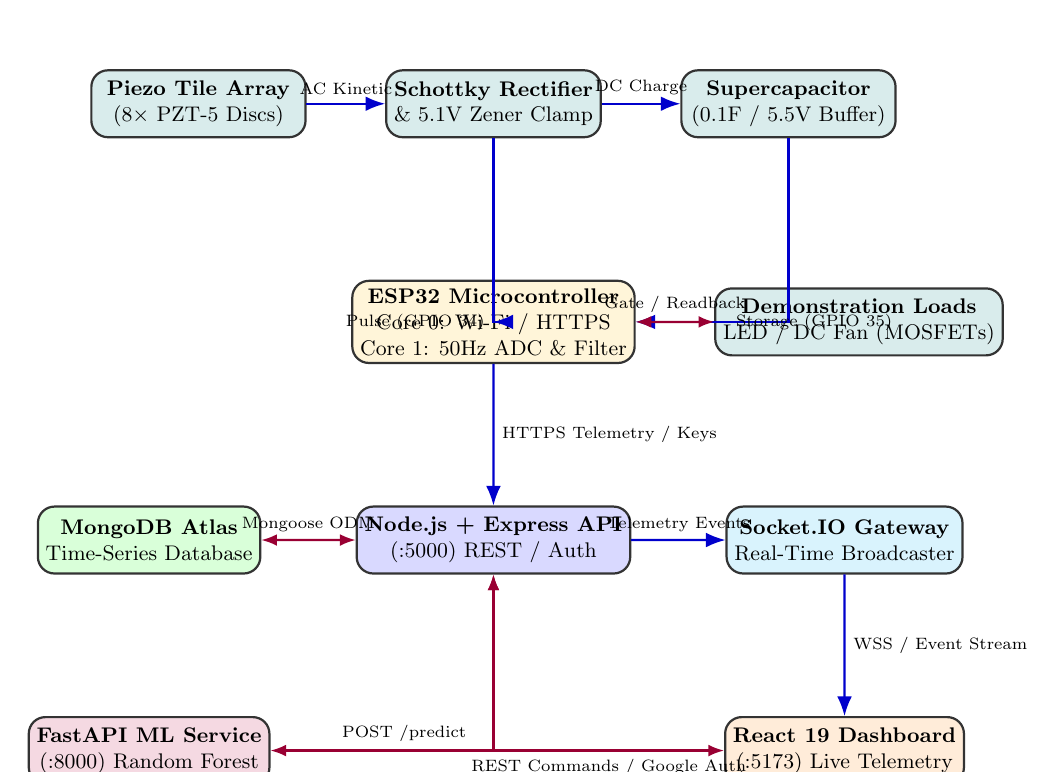
\begin{tikzpicture}[
    scale=0.85, every node/.style={scale=0.85},
    node distance=1.5cm,
    block/.style={rectangle, rounded corners=6pt, draw=black!80, thick, fill=blue!8, align=center, minimum width=3.2cm, minimum height=1.0cm, font=\small},
    subblock/.style={rectangle, rounded corners=4pt, draw=black!70, fill=white, align=center, minimum width=2.8cm, minimum height=0.75cm, font=\footnotesize},
    container/.style={rectangle, rounded corners=8pt, draw=black!60, dashed, thick, fill=gray!5, inner sep=12pt},
    arrow/.style={-{Latex[length=2.5mm]}, thick, draw=blue!80!black},
    darrow/.style={{Latex[length=2mm]}-{Latex[length=2mm]}, thick, draw=purple!80!black}
]
    % Edge Hardware Tier
    \node (piezo) [block, fill=teal!15] {\textbf{Piezo Tile Array}\\(8$\times$ PZT-5 Discs)};
    \node (rect) [block, fill=teal!15, right=1.0cm of piezo] {\textbf{Schottky Rectifier}\\\& 5.1V Zener Clamp};
    \node (cap) [block, fill=teal!15, right=1.0cm of rect] {\textbf{Supercapacitor}\\(0.1F / 5.5V Buffer)};

    % Embedded Tier
    \node (esp) [block, fill=amber!15, below=1.8cm of rect] {\textbf{ESP32 Microcontroller}\\Core 0: Wi-Fi / HTTPS\\Core 1: 50Hz ADC \& Filter};
    \node (loads) [block, fill=teal!15, right=1.0cm of esp] {\textbf{Demonstration Loads}\\LED / DC Fan (MOSFETs)};

    % Cloud Backend Tier
    \node (backend) [block, fill=blue!15, below=1.8cm of esp] {\textbf{Node.js + Express API}\\(:5000) REST / Auth};
    \node (mongo) [block, fill=green!15, left=1.2cm of backend] {\textbf{MongoDB Atlas}\\Time-Series Database};
    \node (socket) [block, fill=cyan!15, right=1.2cm of backend] {\textbf{Socket.IO Gateway}\\Real-Time Broadcaster};

    % ML and Frontend Tier
    \node (ml) [block, fill=purple!15, below=1.8cm of mongo] {\textbf{FastAPI ML Service}\\(:8000) Random Forest};
    \node (frontend) [block, fill=orange!15, below=1.8cm of socket] {\textbf{React 19 Dashboard}\\(:5173) Live Telemetry};

    % Connecting Arrows
    \draw [arrow] (piezo) -- node [above, font=\scriptsize] {AC Kinetic} (rect);
    \draw [arrow] (rect) -- node [above, font=\scriptsize] {DC Charge} (cap);
    \draw [arrow] (rect) |- node [left, pos=0.7, font=\scriptsize] {Pulse (GPIO 34)} (esp);
    \draw [arrow] (cap) |- node [right, pos=0.7, font=\scriptsize] {Storage (GPIO 35)} (esp);
    \draw [darrow] (esp) -- node [above, font=\scriptsize] {Gate / Readback} (loads);

    \draw [arrow] (esp) -- node [right, font=\scriptsize] {HTTPS Telemetry / Keys} (backend);
    \draw [darrow] (backend) -- node [above, font=\scriptsize] {Mongoose ODM} (mongo);
    \draw [arrow] (backend) -- node [above, font=\scriptsize] {Telemetry Events} (socket);

    \draw [darrow] (backend) |- node [above, pos=0.7, font=\scriptsize] {POST /predict} (ml);
    \draw [arrow] (socket) -- node [right, font=\scriptsize] {WSS / Event Stream} (frontend);
    \draw [darrow] (frontend) -| node [below, pos=0.25, font=\scriptsize] {REST Commands / Google Auth} (backend);

\end{tikzpicture}
\caption{Overall StepCharge AI multi-tier cyber-physical system architecture.}
\label{fig:system_architecture}
\end{figure}

The architecture ensures that analog sensing and power conditioning remain completely decoupled from high-level cloud services. Even during transient network outages, local energy accumulation and step detection continue uninterrupted on the edge hardware.

\section{Overall Hardware Architecture}
The hardware subsystem integrates kinetic energy harvesting, analog conditioning, digital processing, and power switching. Figure~\ref{fig:hardware_block_diagram} provides a structural block diagram of the physical components.

\begin{figure}[H]
\centering
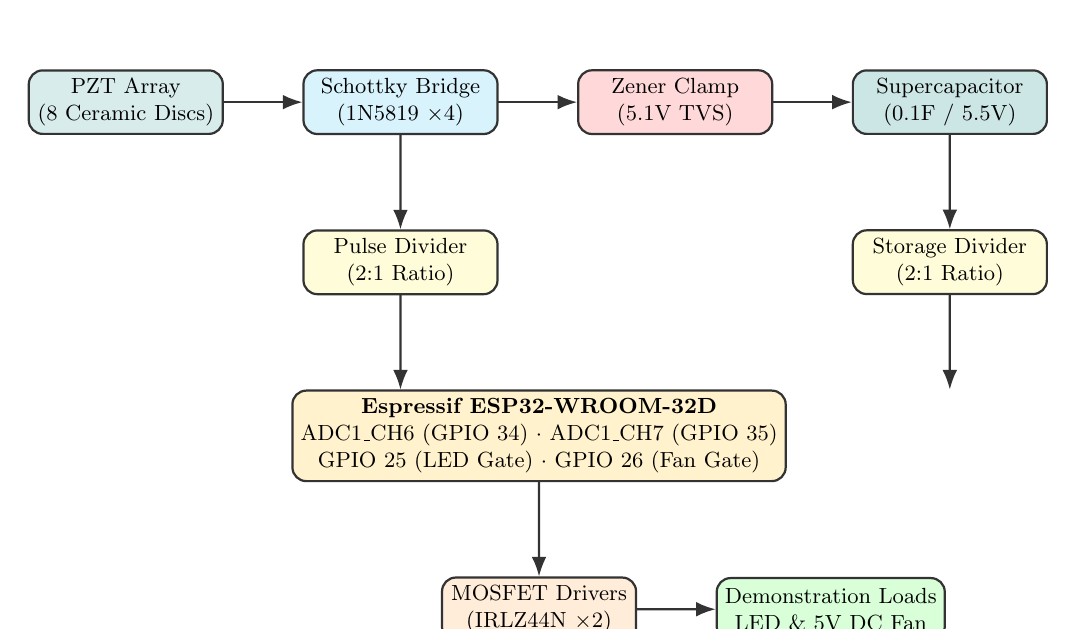
\begin{tikzpicture}[
    scale=0.88, every node/.style={scale=0.88},
    block/.style={rectangle, rounded corners=5pt, draw=black!80, thick, fill=blue!8, align=center, minimum width=2.8cm, minimum height=0.9cm, font=\small},
    arrow/.style={-{Latex[length=2.5mm]}, thick, draw=black!80}
]
    \node (p1) [block, fill=teal!15] {PZT Array\\(8 Ceramic Discs)};
    \node (rec) [block, fill=cyan!15, right=1.0cm of p1] {Schottky Bridge\\(1N5819 $\times$4)};
    \node (tvs) [block, fill=red!15, right=1.0cm of rec] {Zener Clamp\\(5.1V TVS)};
    \node (cap) [block, fill=teal!20, right=1.0cm of tvs] {Supercapacitor\\(0.1F / 5.5V)};

    \node (div1) [block, fill=yellow!15, below=1.2cm of rec] {Pulse Divider\\(2:1 Ratio)};
    \node (div2) [block, fill=yellow!15, below=1.2cm of cap] {Storage Divider\\(2:1 Ratio)};

    \node (esp) [block, fill=amber!20, minimum width=5.5cm, below=1.2cm of div1, xshift=2.0cm] {\textbf{Espressif ESP32-WROOM-32D}\\ADC1\_CH6 (GPIO 34) $\cdot$ ADC1\_CH7 (GPIO 35)\\GPIO 25 (LED Gate) $\cdot$ GPIO 26 (Fan Gate)};

    \node (mos) [block, fill=orange!15, below=1.2cm of esp] {MOSFET Drivers\\(IRLZ44N $\times$2)};
    \node (load) [block, fill=green!15, right=1.0cm of mos] {Demonstration Loads\\LED \& 5V DC Fan};

    \draw [arrow] (p1) -- (rec);
    \draw [arrow] (rec) -- (tvs);
    \draw [arrow] (tvs) -- (cap);
    \draw [arrow] (rec) -- (div1);
    \draw [arrow] (cap) -- (div2);
    \draw [arrow] (div1) -- (esp.north -| div1);
    \draw [arrow] (div2) -- (esp.north -| div2);
    \draw [arrow] (esp) -- (mos);
    \draw [arrow] (mos) -- (load);

\end{tikzpicture}
\caption{Detailed hardware block diagram of the StepCharge AI edge harvesting node.}
\label{fig:hardware_block_diagram}
\end{figure}

\section{Piezoelectric Energy Harvesting Subsystem}
The harvesting array consists of 8 commercial 35\,mm circular Lead Zirconate Titanate (PZT-5) diaphragm elements mounted onto flexible brass backing plates. The transducers are wired in a series-parallel matrix ($2 \times 4$) embedded within an elastomeric polyurethane frame beneath a rigid $300\,\text{mm} \times 300\,\text{mm}$ acrylic top plate. When a footstep impact lands on the plate, mechanical force is distributed across the ceramic elements, inducing dynamic flexural bending and generating simultaneous charge outputs.

\section{Rectifier and Power Conditioning Circuit}
Because piezoelectric transducers generate bipolar alternating current (AC), rectification is mandatory. Figure~\ref{fig:circuit_diagram} depicts the electrical circuit schematic of the conditioning and measurement stages.

\begin{figure}[H]
\centering
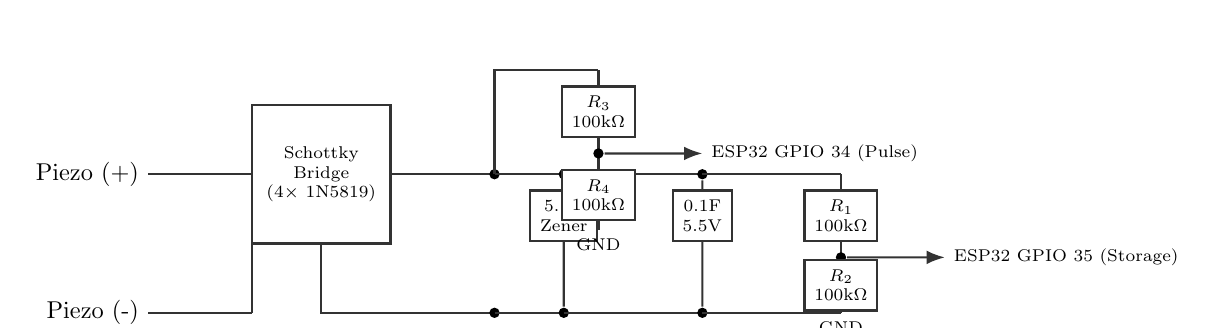
\begin{tikzpicture}[
    scale=0.88, every node/.style={scale=0.88},
    circuit/.style={draw=black!80, thick},
    comp/.style={rectangle, draw=black!80, thick, fill=white, align=center, inner sep=4pt, font=\scriptsize}
]
    % Input from Piezo
    \draw [circuit] (0,2) node[left] {Piezo (+)} -- (1.5,2);
    \draw [circuit] (0,0) node[left] {Piezo (-)} -- (1.5,0);

    % Bridge Rectifier
    \draw [circuit] (1.5,1) rectangle (3.5,3) node[pos=0.5, font=\scriptsize, align=center] {Schottky\\Bridge\\(4$\times$ 1N5819)};
    \draw [circuit] (1.5,2) -- (1.5,1);
    \draw [circuit] (1.5,0) |- (2.5,1);

    % Rectified Output
    \draw [circuit] (3.5,2) -- (5.0,2) node[circle, fill=black, inner sep=1.5pt] (p1) {};
    \draw [circuit] (2.5,1) |- (5.0,0) node[circle, fill=black, inner sep=1.5pt] (g1) {};

    % Zener / TVS Clamp
    \draw [circuit] (5.0,2) -- (6.0,2) node[circle, fill=black, inner sep=1.5pt] (p2) {};
    \draw [circuit] (5.0,0) -- (6.0,0) node[circle, fill=black, inner sep=1.5pt] (g2) {};
    \draw [circuit] (p2) -- (6.0,1.4) node[comp] {5.1V\\Zener} -- (g2);

    % Supercapacitor
    \draw [circuit] (6.0,2) -- (8.0,2) node[circle, fill=black, inner sep=1.5pt] (p3) {};
    \draw [circuit] (6.0,0) -- (8.0,0) node[circle, fill=black, inner sep=1.5pt] (g3) {};
    \draw [circuit] (p3) -- (8.0,1.4) node[comp] {0.1F\\5.5V} -- (g3);

    % Voltage Divider to ADC (Storage)
    \draw [circuit] (8.0,2) -- (10.0,2);
    \draw [circuit] (10.0,2) -- (10.0,1.4) node[comp] {$R_1$\\$100\text{k}\Omega$} -- (10.0,0.8) node[circle, fill=black, inner sep=1.5pt] (adc2) {} -- (10.0,0.4) node[comp] {$R_2$\\$100\text{k}\Omega$} -- (10.0,0);
    \draw [circuit] (8.0,0) -- (10.0,0) node[below, font=\scriptsize] {GND};
    \draw [circuit, -{Latex}] (adc2) -- (11.5,0.8) node[right, font=\scriptsize] {ESP32 GPIO 35 (Storage)};

    % Pulse Divider (Tap from Rectified rail)
    \draw [circuit] (5.0,2) |- (5.0,3.5) -- (6.5,3.5);
    \draw [circuit] (6.5,3.5) -- (6.5,2.9) node[comp] {$R_3$\\$100\text{k}\Omega$} -- (6.5,2.3) node[circle, fill=black, inner sep=1.5pt] (adc1) {} -- (6.5,1.7) node[comp] {$R_4$\\$100\text{k}\Omega$} -- (6.5,1.2) node[below, font=\scriptsize] {GND};
    \draw [circuit, -{Latex}] (adc1) -- (8.0,2.3) node[right, font=\scriptsize] {ESP32 GPIO 34 (Pulse)};

\end{tikzpicture}
\caption{Electrical schematic of rectification, clamping, supercapacitor, and divider sensing.}
\label{fig:circuit_diagram}
\end{figure}

The Schottky diodes (1N5819) exhibit an ultra-low forward-voltage drop ($V_F \approx 0.35\,\text{V}$), conserving scarce micro-energy during low-velocity footfalls. A 5.1\,V Zener clamping diode shunts excessive voltage transients to ground, preventing damage to the supercapacitor buffer and the microcontroller ADC.

\section{Supercapacitor Energy Storage}
Energy accumulation utilizes a 0.1\,F, 5.5\,V Electric Double-Layer Capacitor (EDLC). The total electrical energy stored electrostatically in the capacitor dielectric is given by:
\begin{equation}
E = \frac{1}{2} C V^2
\label{eq:cap_energy}
\end{equation}
where $C = 0.10\,\text{F}$ and $V$ is the terminal voltage. The differential energy accumulated between consecutive footstep cycles is:
\begin{equation}
\Delta E = \frac{1}{2} C \left(V_{\text{final}}^2 - V_{\text{initial}}^2\right)
\label{eq:delta_energy}
\end{equation}

\section{Voltage Measurement Subsystem}
To interface external potentials with the ESP32 ($0.0\text{--}3.3\,\text{V}$ absolute maximum), symmetric $100\,\text{k}\Omega / 100\,\text{k}\Omega$ metal-film resistive dividers are implemented, establishing a scaling ratio of:
\begin{equation}
M = \frac{R_1 + R_2}{R_2} = \frac{100\,\text{k}\Omega + 100\,\text{k}\Omega}{100\,\text{k}\Omega} = 2.0
\label{eq:divider_ratio}
\end{equation}
The true physical voltage $V_{\text{phys}}$ is calculated from the raw 12-bit ADC integer $D \in [0, 4095]$ as:
\begin{equation}
V_{\text{phys}} = \left(\frac{D}{4095.0}\right) \times 3.30\,\text{V} \times 2.0
\label{eq:adc_conversion}
\end{equation}

\section{ESP32 Embedded Monitoring and Signal Acquisition}
The firmware executes a dual-threshold Schmitt trigger to detect valid footsteps. Figure~\ref{fig:schmitt_wave} illustrates the hysteresis detection mechanics.

\begin{figure}[H]
\centering
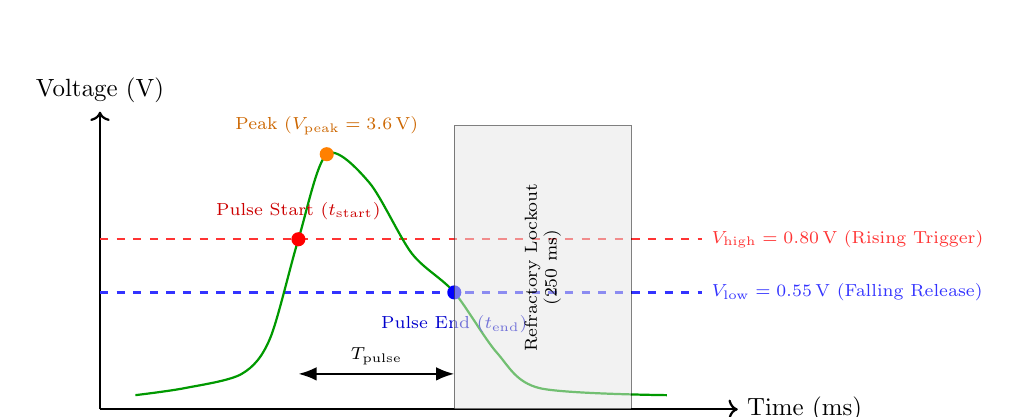
\begin{tikzpicture}[scale=0.9, every node/.style={scale=0.9}]
    \draw [->, thick] (0,0) -- (9.0,0) node [right] {Time (ms)};
    \draw [->, thick] (0,0) -- (0,4.2) node [above] {Voltage (V)};

    % Threshold lines
    \draw [dashed, red!80, thick] (0,2.4) -- (8.5,2.4) node [right, font=\scriptsize] {$V_{\text{high}} = 0.80\,\text{V}$ (Rising Trigger)};
    \draw [dashed, blue!80, thick] (0,1.65) -- (8.5,1.65) node [right, font=\scriptsize] {$V_{\text{low}} = 0.55\,\text{V}$ (Falling Release)};

    % Simulated pulse waveform
    \draw [thick, green!60!black, smooth] plot coordinates {
        (0.5,0.2) (1.2,0.3) (2.0,0.5) (2.4,1.0) (2.8,2.4) (3.2,3.6) (3.8,3.2) (4.4,2.2) (5.0,1.65) (5.6,0.8) (6.2,0.3) (8.0,0.2)
    };

    % Detection Points
    \node at (2.8,2.4) [circle, fill=red, inner sep=2pt] {};
    \node at (2.8,2.8) [font=\scriptsize, red!80!black] {Pulse Start ($t_{\text{start}}$)};

    \node at (5.0,1.65) [circle, fill=blue, inner sep=2pt] {};
    \node at (5.0,1.2) [font=\scriptsize, blue!80!black] {Pulse End ($t_{\text{end}}$)};

    \node at (3.2,3.6) [circle, fill=orange, inner sep=2pt] {};
    \node at (3.2,4.0) [font=\scriptsize, orange!80!black] {Peak ($V_{\text{peak}} = 3.6\,\text{V}$)};

    % Duration Bracket
    \draw [{Latex}-{Latex}, thick] (2.8,0.5) -- (5.0,0.5) node [midway, above, font=\scriptsize] {$T_{\text{pulse}}$};

    % Refractory Window
    \draw [fill=gray!20, opacity=0.5] (5.0,0) rectangle (7.5,4.0);
    \node at (6.25,2.0) [font=\scriptsize, rotate=90, align=center] {Refractory Lockout\\(250 ms)};

\end{tikzpicture}
\caption{Schmitt-trigger hysteresis detection waveform and refractory lockout window.}
\label{fig:schmitt_wave}
\end{figure}

\section{IoT Communication Architecture}
The edge node communicates with the cloud backend via standard TLS-encrypted HTTPS REST protocols. Edge telemetry frames are published every 1000\,ms via \texttt{POST /api/devices/:id/telemetry}. Discrete footsteps are appended via \texttt{POST /api/devices/:id/footsteps}.

\section{Backend Architecture}
The backend service is structured into modular layers:
\begin{itemize}
    \item \textbf{Routing Layer:} Express routers handling \texttt{/api/auth}, \texttt{/api/devices}, \texttt{/api/telemetry}, \texttt{/api/alerts}, and \texttt{/api/ml}.
    \item \textbf{Middleware Layer:} Cryptographic device key validation (\texttt{requireDeviceAuth}), JWT session verification (\texttt{requireAuth}), RBAC enforcement (\texttt{requireAdmin}), rate limiters, and Helmet headers.
    \item \textbf{Service Layer:} Telemetry persistence, health monitoring, and Socket.IO emission.
\end{itemize}

\section{Database Design}
MongoDB Atlas provides document persistence. Relational integrity is enforced programmatically via Mongoose ODM schemas. The primary entity relationships are shown in Section~\ref{sec:er_diagram}.

\section{Machine Learning Architecture}
The machine learning architecture runs as an independent Python FastAPI microservice. The model takes a 5-element feature vector and classifies it via a Random Forest model. Figure~\ref{fig:ml_workflow} illustrates the end-to-end training and inference pipeline.

\begin{figure}[H]
\centering
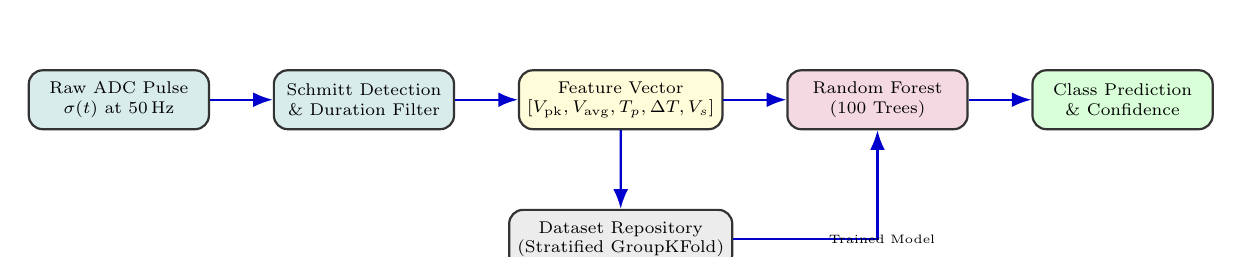
\begin{tikzpicture}[
    scale=0.88, every node/.style={scale=0.88},
    stage/.style={rectangle, rounded corners=5pt, draw=black!80, thick, fill=blue!10, align=center, minimum width=2.6cm, minimum height=0.85cm, font=\scriptsize},
    arrow/.style={-{Latex[length=2.5mm]}, thick, draw=blue!80!black}
]
    \node (raw) [stage, fill=teal!15] {Raw ADC Pulse\\$\sigma(t)$ at 50\,Hz};
    \node (filt) [stage, fill=teal!15, right=0.8cm of raw] {Schmitt Detection\\$\&$ Duration Filter};
    \node (feat) [stage, fill=yellow!15, right=0.8cm of filt] {Feature Vector\\$[V_{\text{pk}}, V_{\text{avg}}, T_p, \Delta T, V_s]$};
    \node (rf) [stage, fill=purple!15, right=0.8cm of feat] {Random Forest\\(100 Trees)};
    \node (out) [stage, fill=green!15, right=0.8cm of rf] {Class Prediction\\\& Confidence};

    \node (db) [stage, fill=gray!15, below=1.0cm of feat] {Dataset Repository\\(Stratified GroupKFold)};

    \draw [arrow] (raw) -- (filt);
    \draw [arrow] (filt) -- (feat);
    \draw [arrow] (feat) -- (rf);
    \draw [arrow] (rf) -- (out);
    \draw [arrow] (feat) -- (db);
    \draw [arrow] (db) -| node [pos=0.3, right, font=\tiny] {Trained Model} (rf);

\end{tikzpicture}
\caption{Machine Learning feature extraction, training, and inference workflow.}
\label{fig:ml_workflow}
\end{figure}

\section{Frontend Dashboard Architecture}
The frontend is constructed using React 19 and TypeScript, structured around a global \texttt{StoreProvider}. A custom hook (\texttt{useStore}) connects to the Socket.IO client, dynamically receiving telemetry frames and updating charts without full re-renders.

\section{Data Flow Diagrams}

\subsection{Data Flow Diagram Level 0 (Context Level)}
Figure~\ref{fig:dfd_level0} illustrates the Level 0 Context DFD representing the highest-level interaction between external entities and the StepCharge AI platform.

\begin{figure}[H]
\centering
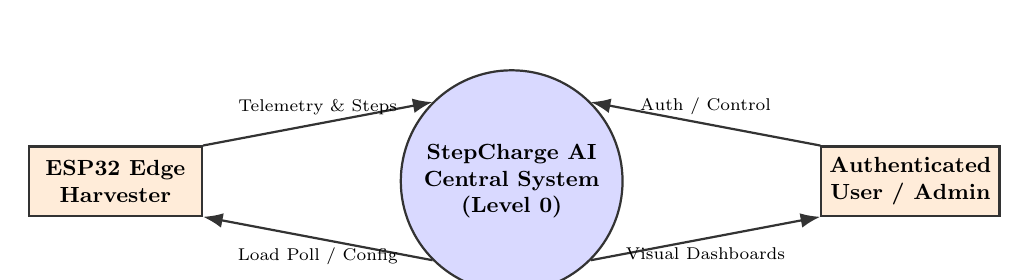
\begin{tikzpicture}[
    scale=0.88, every node/.style={scale=0.88},
    entity/.style={rectangle, draw=black!80, thick, fill=orange!15, align=center, minimum width=2.5cm, minimum height=1.0cm, font=\small\bfseries},
    process/.style={circle, draw=black!80, thick, fill=blue!15, align=center, minimum size=3.2cm, font=\small\bfseries},
    arrow/.style={-{Latex[length=2.5mm]}, thick, draw=black!80}
]
    \node (esp) [entity] {ESP32 Edge\\Harvester};
    \node (sys) [process, right=2.5cm of esp] {StepCharge AI\\Central System\\(Level 0)};
    \node (user) [entity, right=2.5cm of sys] {Authenticated\\User / Admin};

    \draw [arrow] (esp.north east) -- node [above, font=\scriptsize] {Telemetry \& Steps} (sys.north west);
    \draw [arrow] (sys.south west) -- node [below, font=\scriptsize] {Load Poll / Config} (esp.south east);

    \draw [arrow] (user.north west) -- node [above, font=\scriptsize] {Auth / Control} (sys.north east);
    \draw [arrow] (sys.south east) -- node [below, font=\scriptsize] {Visual Dashboards} (user.south west);

\end{tikzpicture}
\caption{Data Flow Diagram (DFD) Level 0 --- Context Level Diagram.}
\label{fig:dfd_level0}
\end{figure}

\subsection{Data Flow Diagram Level 1}
Figure~\ref{fig:dfd_level1} decomposes the system into discrete functional processes, illustrating data stores and internal data paths.

\begin{figure}[H]
\centering
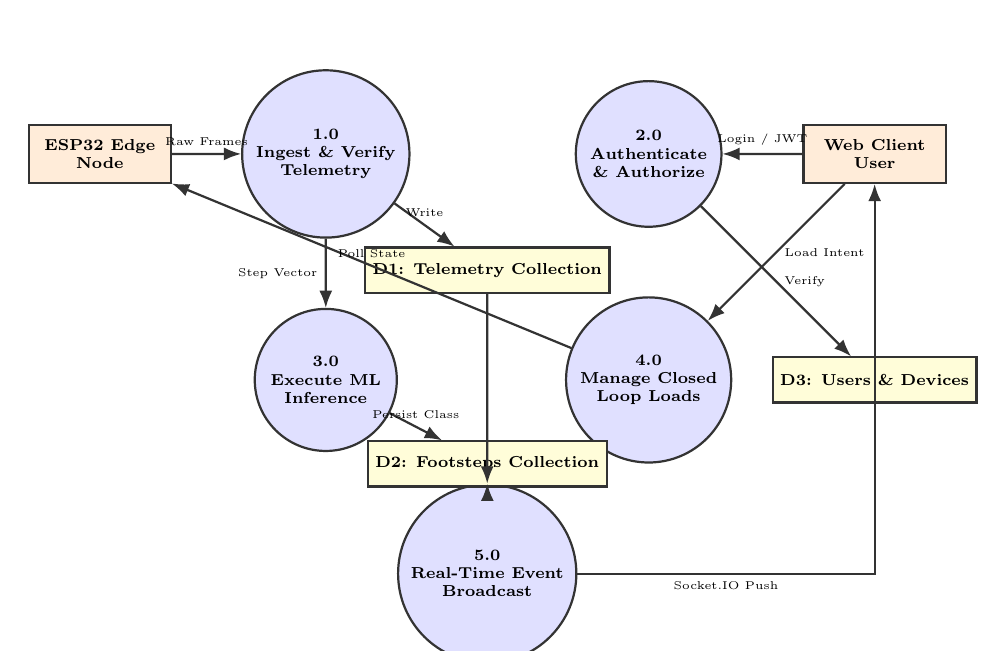
\begin{tikzpicture}[
    scale=0.82, every node/.style={scale=0.82},
    entity/.style={rectangle, draw=black!80, thick, fill=orange!15, align=center, minimum width=2.2cm, minimum height=0.9cm, font=\scriptsize\bfseries},
    proc/.style={circle, draw=black!80, thick, fill=blue!12, align=center, minimum size=2.2cm, font=\scriptsize\bfseries},
    store/.style={rectangle, draw=black!80, thick, fill=yellow!15, minimum width=2.6cm, minimum height=0.7cm, font=\scriptsize\bfseries},
    arrow/.style={-{Latex[length=2.2mm]}, thick, draw=black!80}
]
    % Entities
    \node (esp) [entity] at (0, 6) {ESP32 Edge\\Node};
    \node (user) [entity] at (12, 6) {Web Client\\User};

    % Processes
    \node (p1) [proc] at (3.5, 6) {1.0\\Ingest \& Verify\\Telemetry};
    \node (p2) [proc] at (8.5, 6) {2.0\\Authenticate\\\& Authorize};
    \node (p3) [proc] at (3.5, 2.5) {3.0\\Execute ML\\Inference};
    \node (p4) [proc] at (8.5, 2.5) {4.0\\Manage Closed\\Loop Loads};
    \node (p5) [proc] at (6.0, -0.5) {5.0\\Real-Time Event\\Broadcast};

    % Data Stores
    \node (d1) [store] at (6.0, 4.2) {D1: Telemetry Collection};
    \node (d2) [store] at (6.0, 1.2) {D2: Footsteps Collection};
    \node (d3) [store] at (12, 2.5) {D3: Users \& Devices};

    % Data Flows
    \draw [arrow] (esp) -- node [above, font=\tiny] {Raw Frames} (p1);
    \draw [arrow] (p1) -- node [above, font=\tiny] {Write} (d1);
    \draw [arrow] (p1) -- node [left, font=\tiny] {Step Vector} (p3);
    \draw [arrow] (p3) -- node [above, font=\tiny] {Persist Class} (d2);
    \draw [arrow] (user) -- node [above, font=\tiny] {Login / JWT} (p2);
    \draw [arrow] (p2) -- node [right, font=\tiny] {Verify} (d3);
    \draw [arrow] (user) -- node [right, font=\tiny] {Load Intent} (p4);
    \draw [arrow] (p4) -- node [above, font=\tiny] {Poll State} (esp);
    \draw [arrow] (d1) -- (p5);
    \draw [arrow] (d2) -- (p5);
    \draw [arrow] (p5) -| node [below, pos=0.25, font=\tiny] {Socket.IO Push} (user);

\end{tikzpicture}
\caption{Data Flow Diagram (DFD) Level 1 --- Functional Process Decomposition.}
\label{fig:dfd_level1}
\end{figure}

\section{Entity Relationship Diagram}
\label{sec:er_diagram}
Figure~\ref{fig:er_diagram} presents the Entity-Relationship (ER) model defining the primary collections, attributes, and cardinality in MongoDB Atlas.

\begin{figure}[H]
\centering
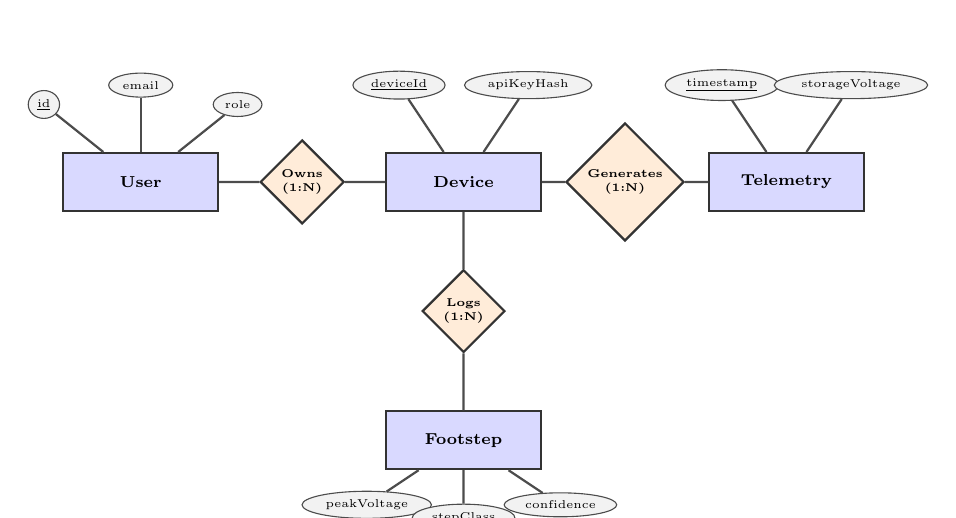
\begin{tikzpicture}[
    scale=0.82, every node/.style={scale=0.82},
    entity/.style={rectangle, draw=black!80, thick, fill=blue!15, align=center, minimum width=2.4cm, minimum height=0.9cm, font=\scriptsize\bfseries},
    attr/.style={ellipse, draw=black!70, fill=gray!10, align=center, font=\tiny, inner sep=2pt},
    rel/.style={diamond, draw=black!80, thick, fill=orange!15, align=center, font=\tiny\bfseries, inner sep=2pt},
    line/.style={thick, draw=black!70}
]
    % Entities
    \node (user) [entity] at (0, 4) {User};
    \node (dev) [entity] at (5, 4) {Device};
    \node (telem) [entity] at (10, 4) {Telemetry};
    \node (step) [entity] at (5, 0) {Footstep};

    % Relationships
    \node (r1) [rel] at (2.5, 4) {Owns\\(1:N)};
    \node (r2) [rel] at (7.5, 4) {Generates\\(1:N)};
    \node (r3) [rel] at (5, 2) {Logs\\(1:N)};

    % Connecting lines
    \draw [line] (user) -- (r1) -- (dev);
    \draw [line] (dev) -- (r2) -- (telem);
    \draw [line] (dev) -- (r3) -- (step);

    % Attributes for User
    \node (u1) [attr] at (-1.5, 5.2) {\underline{id}};
    \node (u2) [attr] at (0, 5.5) {email};
    \node (u3) [attr] at (1.5, 5.2) {role};
    \draw [line] (user) -- (u1); \draw [line] (user) -- (u2); \draw [line] (user) -- (u3);

    % Attributes for Device
    \node (d1) [attr] at (4.0, 5.5) {\underline{deviceId}};
    \node (d2) [attr] at (6.0, 5.5) {apiKeyHash};
    \draw [line] (dev) -- (d1); \draw [line] (dev) -- (d2);

    % Attributes for Telemetry
    \node (t1) [attr] at (9.0, 5.5) {\underline{timestamp}};
    \node (t2) [attr] at (11.0, 5.5) {storageVoltage};
    \draw [line] (telem) -- (t1); \draw [line] (telem) -- (t2);

    % Attributes for Footstep
    \node (s1) [attr] at (3.5, -1.0) {peakVoltage};
    \node (s2) [attr] at (5.0, -1.2) {stepClass};
    \node (s3) [attr] at (6.5, -1.0) {confidence};
    \draw [line] (step) -- (s1); \draw [line] (step) -- (s2); \draw [line] (step) -- (s3);

\end{tikzpicture}
\caption{Entity-Relationship (ER) diagram representing the MongoDB Atlas schema.}
\label{fig:er_diagram}
\end{figure}

\section{Unified Modeling Language (UML) Diagrams}

\subsection{Use Case Diagram}
Figure~\ref{fig:use_case} depicts system interactions from the perspective of two primary actors: the Pedestrian (who imparts mechanical stress) and the Authenticated System User / Admin (who monitors and manages the system).

\begin{figure}[H]
\centering
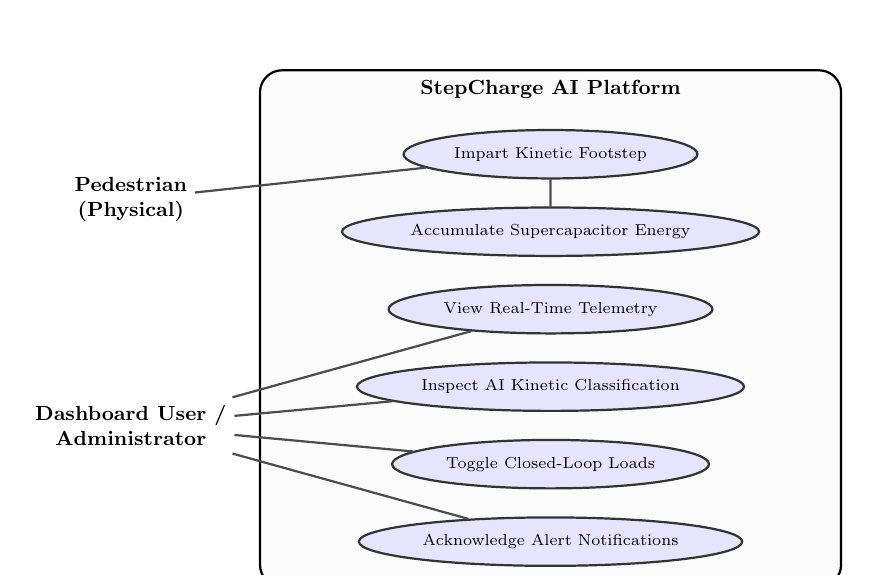
\begin{tikzpicture}[
    scale=0.82, every node/.style={scale=0.82},
    actor/.style={rectangle, draw=none, font=\small\bfseries, align=center},
    uc/.style={ellipse, draw=black!80, thick, fill=blue!10, align=center, font=\scriptsize, minimum width=3.0cm, minimum height=0.75cm},
    arrow/.style={thick, draw=black!70}
]
    % System boundary
    \draw [thick, rounded corners=8pt, fill=gray!3] (-1.0, -4.5) rectangle (8.0, 3.5);
    \node at (3.5, 3.2) [font=\small\bfseries] {StepCharge AI Platform};

    % Actors
    \node (ped) [actor] at (-3.0, 1.5) {Pedestrian\\(Physical)};
    \node (user) [actor] at (-3.0, -2.0) {Dashboard User /\\Administrator};

    % Use Cases
    \node (uc1) [uc] at (3.5, 2.2) {Impart Kinetic Footstep};
    \node (uc2) [uc] at (3.5, 1.0) {Accumulate Supercapacitor Energy};
    \node (uc3) [uc] at (3.5, -0.2) {View Real-Time Telemetry};
    \node (uc4) [uc] at (3.5, -1.4) {Inspect AI Kinetic Classification};
    \node (uc5) [uc] at (3.5, -2.6) {Toggle Closed-Loop Loads};
    \node (uc6) [uc] at (3.5, -3.8) {Acknowledge Alert Notifications};

    % Links
    \draw [arrow] (ped) -- (uc1);
    \draw [arrow] (uc1) -- (uc2);
    \draw [arrow] (user) -- (uc3);
    \draw [arrow] (user) -- (uc4);
    \draw [arrow] (user) -- (uc5);
    \draw [arrow] (user) -- (uc6);

\end{tikzpicture}
\caption{Use Case Diagram modeling user and physical actor interactions.}
\label{fig:use_case}
\end{figure}

\subsection{Activity Diagram}
Figure~\ref{fig:activity_diagram} traces the continuous operational lifecycle of edge signal acquisition, Schmitt trigger validation, and telemetry streaming.

\begin{figure}[H]
\centering
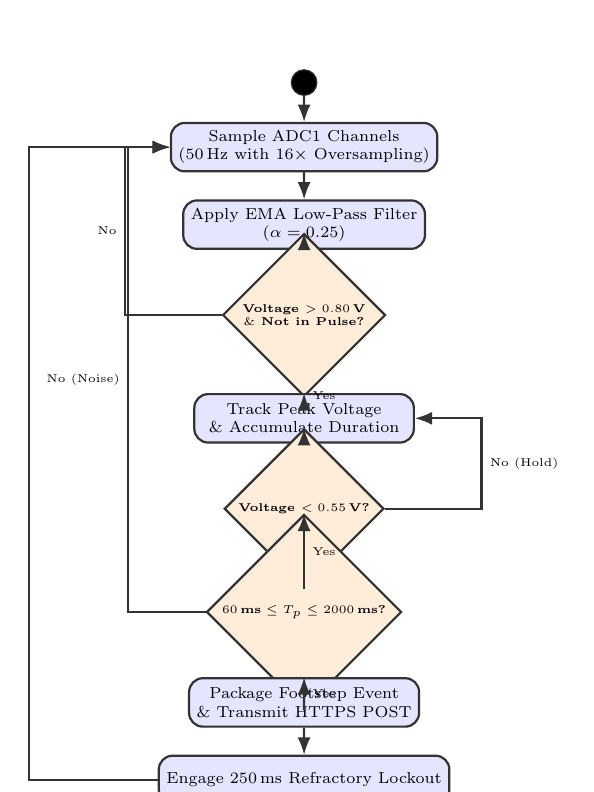
\begin{tikzpicture}[
    scale=0.82, every node/.style={scale=0.82},
    action/.style={rectangle, rounded corners=5pt, draw=black!80, thick, fill=blue!10, align=center, minimum width=3.4cm, minimum height=0.75cm, font=\scriptsize},
    dec/.style={diamond, draw=black!80, thick, fill=orange!15, align=center, font=\tiny\bfseries, inner sep=2pt},
    startstop/.style={circle, draw=black!80, fill=black, inner sep=4pt},
    endstop/.style={circle, draw=black!80, double, fill=black, inner sep=3pt},
    arrow/.style={-{Latex[length=2.2mm]}, thick, draw=black!80}
]
    \node (start) [startstop] at (0, 7) {};
    \node (sample) [action] at (0, 6.0) {Sample ADC1 Channels\\(50\,Hz with 16$\times$ Oversampling)};
    \node (ema) [action] at (0, 4.8) {Apply EMA Low-Pass Filter\\($\alpha = 0.25$)};
    \node (d1) [dec] at (0, 3.4) {Voltage $> 0.80\,\text{V}$\\$\&$ Not in Pulse?};
    \node (pulse) [action] at (0, 1.8) {Track Peak Voltage\\$\&$ Accumulate Duration};
    \node (d2) [dec] at (0, 0.4) {Voltage $< 0.55\,\text{V}$?};
    \node (valid) [dec] at (0, -1.2) {$60\,\text{ms} \le T_p \le 2000\,\text{ms}$?};
    \node (tx) [action] at (0, -2.6) {Package Footstep Event\\\& Transmit HTTPS POST};
    \node (refr) [action] at (0, -3.8) {Engage 250\,ms Refractory Lockout};

    \draw [arrow] (start) -- (sample);
    \draw [arrow] (sample) -- (ema);
    \draw [arrow] (ema) -- (d1);
    \draw [arrow] (d1) -- node [right, font=\tiny] {Yes} (pulse);
    \draw [arrow] (d1.west) -- ++(-1.5,0) |- node [left, pos=0.25, font=\tiny] {No} (sample.west);
    \draw [arrow] (pulse) -- (d2);
    \draw [arrow] (d2) -- node [right, font=\tiny] {Yes} (valid);
    \draw [arrow] (d2.east) -- ++(1.5,0) |- node [right, pos=0.25, font=\tiny] {No (Hold)} (pulse.east);
    \draw [arrow] (valid) -- node [right, font=\tiny] {Yes} (tx);
    \draw [arrow] (valid.west) -- ++(-1.2,0) |- node [left, pos=0.25, font=\tiny] {No (Noise)} (sample.west);
    \draw [arrow] (tx) -- (refr);
    \draw [arrow] (refr.west) -- ++(-2.0,0) |- (sample.west);

\end{tikzpicture}
\caption{Activity Diagram illustrating the edge firmware step detection and telemetry cycle.}
\label{fig:activity_diagram}
\end{figure}

\subsection{State Machine Diagram}
Figure~\ref{fig:state_diagram} represents the operational states of the ESP32 edge microcontroller.

\begin{figure}[H]
\centering
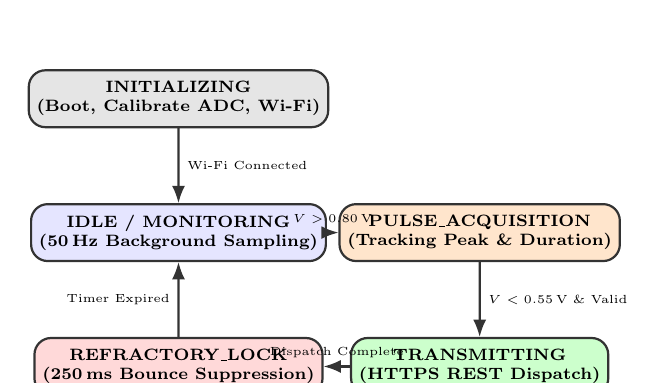
\begin{tikzpicture}[
    scale=0.85, every node/.style={scale=0.85},
    state/.style={rectangle, rounded corners=6pt, draw=black!80, thick, fill=blue!10, align=center, minimum width=3.0cm, minimum height=0.85cm, font=\scriptsize\bfseries},
    arrow/.style={-{Latex[length=2.2mm]}, thick, draw=black!80}
]
    \node (init) [state, fill=gray!20] at (0, 4) {INITIALIZING\\(Boot, Calibrate ADC, Wi-Fi)};
    \node (idle) [state] at (0, 2) {IDLE / MONITORING\\(50\,Hz Background Sampling)};
    \node (pulse) [state, fill=orange!20] at (4.5, 2) {PULSE\_ACQUISITION\\(Tracking Peak \& Duration)};
    \node (tx) [state, fill=green!20] at (4.5, 0) {TRANSMITTING\\(HTTPS REST Dispatch)};
    \node (lock) [state, fill=red!15] at (0, 0) {REFRACTORY\_LOCK\\(250\,ms Bounce Suppression)};

    \draw [arrow] (init) -- node [right, font=\tiny] {Wi-Fi Connected} (idle);
    \draw [arrow] (idle) -- node [above, font=\tiny] {$V > 0.80\,\text{V}$} (pulse);
    \draw [arrow] (pulse) -- node [right, font=\tiny] {$V < 0.55\,\text{V}$ \& Valid} (tx);
    \draw [arrow] (tx) -- node [above, font=\tiny] {Dispatch Complete} (lock);
    \draw [arrow] (lock) -- node [left, font=\tiny] {Timer Expired} (idle);

\end{tikzpicture}
\caption{State Machine Diagram of the ESP32 edge firmware.}
\label{fig:state_diagram}
\end{figure}

\subsection{Class Diagram}
Figure~\ref{fig:class_diagram} outlines the object-oriented structure of backend models and controllers.

\begin{figure}[H]
\centering
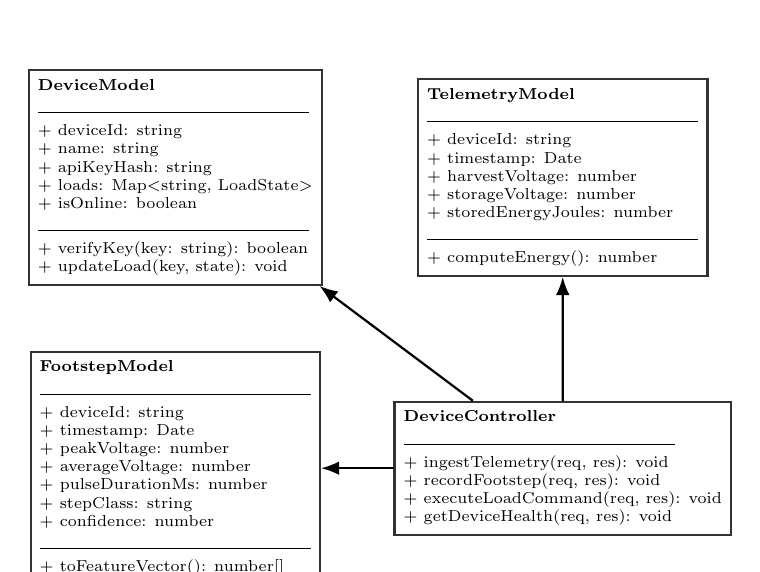
\begin{tikzpicture}[
    scale=0.82, every node/.style={scale=0.82},
    class/.style={rectangle, draw=black!80, thick, fill=white, align=left, font=\scriptsize, inner sep=4pt}
]
    \node (dev) [class] at (0, 4) {
        \textbf{DeviceModel}\\[2pt]
        \rule{4.2cm}{0.4pt}\\[2pt]
        + deviceId: string\\
        + name: string\\
        + apiKeyHash: string\\
        + loads: Map$<$string, LoadState$>$\\
        + isOnline: boolean\\[2pt]
        \rule{4.2cm}{0.4pt}\\[2pt]
        + verifyKey(key: string): boolean\\
        + updateLoad(key, state): void
    };

    \node (telem) [class] at (6.0, 4) {
        \textbf{TelemetryModel}\\[2pt]
        \rule{4.2cm}{0.4pt}\\[2pt]
        + deviceId: string\\
        + timestamp: Date\\
        + harvestVoltage: number\\
        + storageVoltage: number\\
        + storedEnergyJoules: number\\[2pt]
        \rule{4.2cm}{0.4pt}\\[2pt]
        + computeEnergy(): number
    };

    \node (step) [class] at (0, -0.5) {
        \textbf{FootstepModel}\\[2pt]
        \rule{4.2cm}{0.4pt}\\[2pt]
        + deviceId: string\\
        + timestamp: Date\\
        + peakVoltage: number\\
        + averageVoltage: number\\
        + pulseDurationMs: number\\
        + stepClass: string\\
        + confidence: number\\[2pt]
        \rule{4.2cm}{0.4pt}\\[2pt]
        + toFeatureVector(): number[]
    };

    \node (ctrl) [class] at (6.0, -0.5) {
        \textbf{DeviceController}\\[2pt]
        \rule{4.2cm}{0.4pt}\\[2pt]
        + ingestTelemetry(req, res): void\\
        + recordFootstep(req, res): void\\
        + executeLoadCommand(req, res): void\\
        + getDeviceHealth(req, res): void
    };

    \draw [thick, -{Latex}] (ctrl) -- (dev);
    \draw [thick, -{Latex}] (ctrl) -- (telem);
    \draw [thick, -{Latex}] (ctrl) -- (step);

\end{tikzpicture}
\caption{Class Diagram illustrating primary backend models and services.}
\label{fig:class_diagram}
\end{figure}

\subsection{Sequence Diagram}
Figure~\ref{fig:sequence_diagram} models the interaction sequence during footstep detection, ML inferencing, and live broadcasting.

\begin{figure}[H]
\centering
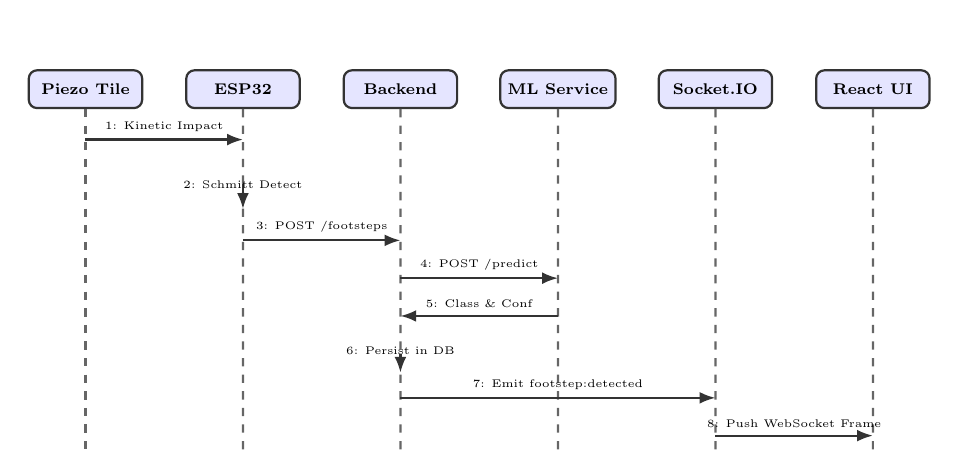
\begin{tikzpicture}[
    scale=0.80, every node/.style={scale=0.80},
    lifeline/.style={dashed, draw=black!60, thick},
    obj/.style={rectangle, rounded corners=3pt, draw=black!80, thick, fill=blue!10, align=center, font=\scriptsize\bfseries, minimum width=1.8cm, minimum height=0.6cm},
    msg/.style={-{Latex[length=2mm]}, thick, draw=black!80, font=\tiny}
]
    % Entities
    \node (p) [obj] at (0, 6) {Piezo Tile};
    \node (e) [obj] at (2.5, 6) {ESP32};
    \node (b) [obj] at (5.0, 6) {Backend};
    \node (m) [obj] at (7.5, 6) {ML Service};
    \node (s) [obj] at (10.0, 6) {Socket.IO};
    \node (u) [obj] at (12.5, 6) {React UI};

    % Lifelines
    \draw [lifeline] (p) -- (0, 0);
    \draw [lifeline] (e) -- (2.5, 0);
    \draw [lifeline] (b) -- (5.0, 0);
    \draw [lifeline] (m) -- (7.5, 0);
    \draw [lifeline] (s) -- (10.0, 0);
    \draw [lifeline] (u) -- (12.5, 0);

    % Messages
    \draw [msg] (0, 5.2) -- node [above] {1: Kinetic Impact} (2.5, 5.2);
    \draw [msg] (2.5, 4.5) -- node [above] {2: Schmitt Detect} (2.5, 4.1);
    \draw [msg] (2.5, 3.6) -- node [above] {3: POST /footsteps} (5.0, 3.6);
    \draw [msg] (5.0, 3.0) -- node [above] {4: POST /predict} (7.5, 3.0);
    \draw [msg] (7.5, 2.4) -- node [above] {5: Class \& Conf} (5.0, 2.4);
    \draw [msg] (5.0, 1.8) -- node [above] {6: Persist in DB} (5.0, 1.5);
    \draw [msg] (5.0, 1.1) -- node [above] {7: Emit footstep:detected} (10.0, 1.1);
    \draw [msg] (10.0, 0.5) -- node [above] {8: Push WebSocket Frame} (12.5, 0.5);

\end{tikzpicture}
\caption{Sequence Diagram of footstep acquisition, ML classification, and UI update.}
\label{fig:sequence_diagram}
\end{figure}

\subsection{Object Diagram}
Figure~\ref{fig:object_diagram} depicts a concrete runtime snapshot of system instances during a live testing session.

\begin{figure}[H]
\centering
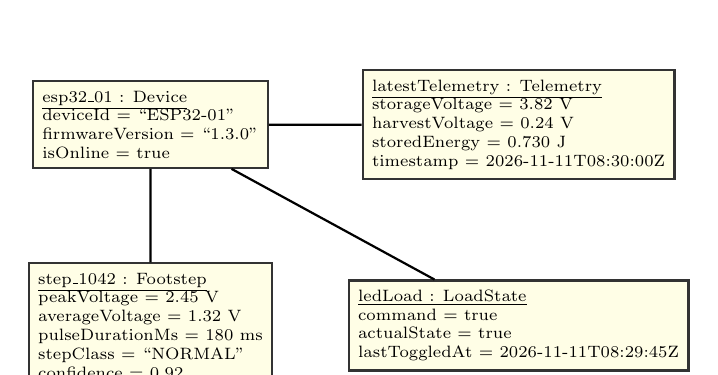
\begin{tikzpicture}[
    scale=0.85, every node/.style={scale=0.85},
    obj/.style={rectangle, draw=black!80, thick, fill=yellow!10, align=left, font=\scriptsize, inner sep=4pt}
]
    \node (dev1) [obj] at (0, 3) {
        \underline{esp32\_01 : Device}\\
        deviceId = ``ESP32-01''\\
        firmwareVersion = ``1.3.0''\\
        isOnline = true
    };

    \node (telem1) [obj] at (5.5, 3) {
        \underline{latestTelemetry : Telemetry}\\
        storageVoltage = 3.82 V\\
        harvestVoltage = 0.24 V\\
        storedEnergy = 0.730 J\\
        timestamp = 2026-11-11T08:30:00Z
    };

    \node (step1) [obj] at (0, 0) {
        \underline{step\_1042 : Footstep}\\
        peakVoltage = 2.45 V\\
        averageVoltage = 1.32 V\\
        pulseDurationMs = 180 ms\\
        stepClass = ``NORMAL''\\
        confidence = 0.92
    };

    \node (load1) [obj] at (5.5, 0) {
        \underline{ledLoad : LoadState}\\
        command = true\\
        actualState = true\\
        lastToggledAt = 2026-11-11T08:29:45Z
    };

    \draw [thick] (dev1) -- (telem1);
    \draw [thick] (dev1) -- (step1);
    \draw [thick] (dev1) -- (load1);

\end{tikzpicture}
\caption{Object Diagram capturing runtime instances during a footstep event.}
\label{fig:object_diagram}
\end{figure}

\chapter{Implementation and Technical Specifications}

\section{Introduction}
The implementation of StepCharge AI translates the theoretical design into a verified, operational cyber-physical system. This chapter details the physical prototyping of the piezoelectric floor tile, embedded C++ firmware routines, cloud REST controllers in TypeScript, MongoDB Atlas schema integration, the Python machine learning inferencing microservice, and the React 19 web dashboard. Furthermore, the chapter documents the security architectures, hardware-software integration loops, and error-handling protocols established across the platform.

\section{Hardware Implementation and Prototyping}
The physical prototype was constructed using an iterative benchtop prototyping methodology. The mechanical structure consists of a sandwich enclosure:
\begin{enumerate}
    \item \textbf{Base Substrate:} A 12\,mm high-density plywood baseplate providing structural rigidity and dampening acoustic reflections from the floor.
    \item \textbf{Transducer Matrix Layer:} Eight 35\,mm Lead Zirconate Titanate (PZT-5) piezoelectric diaphragm discs arranged in a $2 \times 4$ rectangular grid. Each disc is seated on high-resilience silicone O-rings to permit controlled flexural deformation without edge pinning.
    \item \textbf{Impact Transmission Plate:} A 6\,mm transparent polymethyl methacrylate (acrylic) surface plate that distributes the pedestrian's vertical heel-strike load uniformly across the underlying transducers.
    \item \textbf{Perimeter Shock Absorbers:} Neoprene elastomeric foam perimeter gaskets that absorb lateral shear forces and restore the acrylic plate to its neutral equilibrium state following impact release.
\end{enumerate}

\section{Piezoelectric Sensor Integration}
The eight piezoelectric discs are electrically interconnected in a series-parallel configuration. Pairing two discs in series doubles the open-circuit output voltage, while connecting four parallel branches quadruples the aggregate output current. The combined positive and negative terminals are shielded with braided copper sleeving to minimize 50\,Hz electromagnetic interference (EMI) pick-up before routing into the signal conditioning circuit.

\section{Rectification, Conditioning and Supercapacitor Storage}
The conditioning circuit is assembled on a dedicated prototyping printed circuit board (PCB):
\begin{itemize}
    \item \textbf{Rectification:} A full-wave bridge rectifier constructed with four 1N5819 Schottky barrier diodes. The low forward-voltage drop ($V_F \approx 0.35\,\text{V}$) ensures that low-energy footfalls are efficiently rectified.
    \item \textbf{Voltage Clamping:} A 5.1\,V Zener diode (1N4733A) is connected across the rectified DC rail in reverse breakdown configuration, safely clamping voltage spikes exceeding 5.1\,V to protect the supercapacitor and the ESP32.
    \item \textbf{Energy Storage Reservoir:} An electric double-layer supercapacitor rated at 0.1\,F and 5.5\,V is positioned downstream of the rectifier.
    \item \textbf{Sensing Dividers:} Two separate precision resistive dividers ($100\,\text{k}\Omega / 100\,\text{k}\Omega$, metal-film, 1\% tolerance) scale the rectified pulse rail and the supercapacitor terminal voltage by a factor of 2.0.
\end{itemize}

\section{ESP32 Firmware Implementation}
The edge firmware is implemented in C++ using the Arduino-ESP32 core (v2.0.14+). The firmware leverages the ESP32 dual-core Xtensa architecture:
\begin{itemize}
    \item \textbf{Core 0 (Networking Task):} Runs the underlying FreeRTOS TCP/IP stack, Wi-Fi reconnection state machine, and periodic HTTPS REST client requests.
    \item \textbf{Core 1 (Real-Time Sensing Task):} Dedicated to time-critical analog signal sampling, digital filtering, Schmitt-trigger hysteresis tracking, and closed-loop GPIO load control.
\end{itemize}

\section{Sensor Data Acquisition and Calibration}
Analog sampling executes at a deterministic 50\,Hz interval ($20\,\text{ms}$) via high-resolution hardware timers. The sampling pipeline incorporates:
\begin{enumerate}
    \item \textbf{16$\times$ Hardware Oversampling:} Sixteen consecutive analog reads are performed in rapid succession on ADC1\_CH6 (GPIO 34) and ADC1\_CH7 (GPIO 35) and averaged to eliminate random Gaussian quantization noise.
    \item \textbf{Exponential Moving Average (EMA) Smoothing:} The averaged reading is smoothed using the recurrence relation:
    \begin{equation}
    V_{\text{ema}}[k] = V_{\text{ema}}[k-1] + \frac{V_{\text{raw}}[k] - V_{\text{ema}}[k-1]}{4}
    \end{equation}
    which implements a low-pass digital filter with $\alpha = 0.25$, attenuating high-frequency electrical switching spikes.
    \item \textbf{Calibrated Voltage Conversion:} Calibrated reference coefficients scale raw integer values ($0\text{--}4095$) into physical voltages ($V_{\text{phys}} = \frac{D}{4095.0} \times 3.30\,\text{V} \times 2.0$).
\end{enumerate}

\section{Wi-Fi Communication and Secure REST Telemetry}
The ESP32 connects to an encrypted 2.4\,GHz WPA2 Wi-Fi network. Every 1000\,ms, the firmware constructs a structured JSON telemetry frame and dispatches it via an HTTPS POST request:
\begin{lstlisting}[language=C++, caption={JSON telemetry serialization in ESP32 firmware.}, label={lst:firmware_json}]
JsonDocument doc;
doc["storageVoltage"] = lastStorage;
doc["harvestVoltage"] = lastPeak;
doc["storedEnergyJoules"] = 0.5 * 0.10 * lastStorage * lastStorage;
doc["footstepCount"]  = footstepCount;
doc["uptimeSec"]      = millis() / 1000;

String jsonPayload;
serializeJson(doc, jsonPayload);

http.begin(client, SERVER_TELEMETRY_URL);
http.addHeader("Content-Type", "application/json");
http.addHeader("X-Device-Key", DEVICE_SECRET_KEY);
int httpResponseCode = http.POST(jsonPayload);
\end{lstlisting}

\section{Backend API Implementation}
The backend service is engineered in Node.js, Express, and TypeScript. The application architecture enforces modular separation of concerns:
\begin{itemize}
    \item \texttt{/backend/src/controllers/deviceController.ts}: Ingests incoming telemetry, validates physical voltage bounds ($0.0\,\text{V} \le V \le 60.0\,\text{V}$), ensures $V_{\text{avg}} \le V_{\text{peak}}$, and commits records to MongoDB Atlas.
    \item \texttt{/backend/src/controllers/authController.ts}: Manages Google OAuth 2.0 authorization, credential verification, and user session lifecycle.
    \item \texttt{/backend/src/controllers/alertController.ts}: Generates real-time anomaly alerts and manages the ``Mark as Read'' operational flow with complete database persistence.
\end{itemize}

\section{Google Authentication and Role-Based Access Control}
User authentication utilizes Google OAuth 2.0 as the primary identity provider, supplemented by local cryptographic email/password authentication:
\begin{enumerate}
    \item The client initiates authentication via \texttt{GET /api/auth/google/url}, receiving an authorization URL containing a cryptographically random, signed CSRF state token stored in a temporary HttpOnly cookie.
    \item Google redirects back to \texttt{/api/auth/google/callback} with an authorization code.
    \item The backend exchanges the code for Google user identity tokens, retrieves or creates the user in MongoDB Atlas, and generates a signed JSON Web Token (JWT) with a 7-day expiration.
    \item The JWT is set into an \texttt{HttpOnly}, \texttt{SameSite=Lax}, \texttt{Secure} (in production) cookie named \texttt{stepcharge\_session}.
    \item The \texttt{requireAuth} middleware extracts and verifies the cookie on protected endpoints, attaching \texttt{req.user} and enforcing RBAC permissions (\texttt{USER} vs \texttt{ADMIN}).
\end{enumerate}

\section{MongoDB Atlas Integration and Time-Series Optimization}
The MongoDB Atlas database utilizes Mongoose schemas with strict data typing and lifecycle hooks. To ensure sub-millisecond query performance during high-frequency telemetry ingestion, compound indexes are defined:
\begin{lstlisting}[language=Java, caption={Mongoose compound indexing on time-series telemetry.}, label={lst:mongo_index}]
const telemetrySchema = new Schema({
  deviceId: { type: String, required: true, index: true },
  timestamp: { type: Date, required: true, default: Date.now },
  storageVoltage: { type: Number, required: true, min: 0, max: 60 },
  harvestVoltage: { type: Number, required: true, min: 0, max: 60 },
  storedEnergyJoules: { type: Number, required: true },
  linkStats: { rssi: Number, ip: String }
});

telemetrySchema.index({ deviceId: 1, timestamp: -1 });
\end{lstlisting}

\section{Real-Time Communication Using Socket.IO}
Real-time telemetry and event notifications are distributed via Socket.IO v4.7. Clients connect to the server and join device-specific room channels (e.g., \texttt{device:ESP32-01}). When the REST API ingests a valid telemetry frame or footstep impact, it immediately dispatches the event to the designated room:
\begin{lstlisting}[language=Java, caption={Socket.IO device-scoped event emission.}, label={lst:socket_emit}]
io.to(`device:${deviceId}`).emit('telemetry:update', {
  deviceId,
  storageVoltage,
  harvestVoltage,
  storedEnergyJoules,
  timestamp: new Date()
});
\end{lstlisting}

\section{Machine Learning Implementation}
The machine learning pipeline is implemented in Python 3.11 using Scikit-Learn v1.4 and served via FastAPI. The classifier is an ensemble Random Forest (\texttt{RandomForestClassifier}) configured with 100 decision trees, balanced class weighting, and a maximum tree depth of 12 to prevent overfitting.

\section{Data Preprocessing and Feature Extraction}
When a footstep occurs, the system extracts a 5-dimensional physical feature vector:
\begin{enumerate}
    \item \textbf{Peak Voltage ($V_{\text{peak}}$):} Maximum voltage attained during the pulse transient.
    \item \textbf{Average Voltage ($V_{\text{avg}}$):} Arithmetic mean voltage integrated over the pulse duration.
    \item \textbf{Pulse Duration ($T_{\text{pulse}}$):} Temporal width of the pulse in milliseconds from rising trigger to falling release.
    \item \textbf{Cadence Interval ($\Delta T_{\text{step}}$):} Elapsed time in seconds since the conclusion of the preceding footstep.
    \item \textbf{Storage Voltage ($V_{\text{storage}}$):} Real-time voltage on the supercapacitor rail at the moment of impact.
\end{enumerate}

Physical plausibility bounds are strictly enforced. Samples with $V_{\text{peak}} > 60\,\text{V}$, $V_{\text{avg}} > V_{\text{peak}}$, or $T_{\text{pulse}} < 1.0\,\text{ms}$ are flagged as sensor faults and rejected.

\section{Footstep Classification and Subject-Independent Validation}
To eliminate gait identity memorization, model training enforces \texttt{StratifiedGroupKFold} cross-validation ($k = 5$), grouping samples by participant identifier (\texttt{participantId}). This guarantees that all footsteps from any given participant are isolated strictly within either the training partition or the testing partition, preventing identity leakage.

\section{React Dashboard Implementation}
The client dashboard is developed using React 19, TypeScript, and Tailwind CSS. The application architecture features:
\begin{itemize}
    \item \textbf{Live Telemetry Dials:} High-contrast SVG circular gauges rendering storage voltage ($0.0\text{--}5.0\,\text{V}$) and estimated capacitor energy ($0.0\text{--}1.25\,\text{J}$).
    \item \textbf{Time-Series Waveform Charts:} Responsive Recharts components rendering historical voltage transients and moving averages.
    \item \textbf{AI Insights Feed:} Live notification badges displaying the latest classified footstep (\texttt{LIGHT}, \texttt{NORMAL}, \texttt{HEAVY}) alongside confidence percentages and inference latency.
    \item \textbf{Closed-Loop Load Controls:} Interactive toggles for the LED indicator and 5\,V fan that visually reflect an active state only upon confirmed GPIO hardware readback (\texttt{actualState == true}).
    \item \textbf{Accessible Profile Menu:} A dark glass floating panel featuring user identity, email, RBAC role, outside-click detection, and Escape key dismissal.
\end{itemize}

\section{Integration of Hardware and Software}
Hardware and software tiers operate in a closed feedback loop:
\begin{enumerate}
    \item Mechanical footstep impact $\rightarrow$ Piezoelectric charge generated.
    \item Schottky rectification $\rightarrow$ Supercapacitor accumulates charge.
    \item ESP32 Core 1 detects step $\rightarrow$ Caches peak, average, and duration.
    \item ESP32 Core 0 transmits HTTPS POST $\rightarrow$ Node.js backend validates payload.
    \item Backend calls Python ML microservice $\rightarrow$ Predicts gait class.
    \item Backend commits records to MongoDB Atlas $\rightarrow$ Emits Socket.IO event.
    \item React dashboard updates dials and charts in real time ($<100\,\text{ms}$).
    \item User toggles load on UI $\rightarrow$ ESP32 switches MOSFET $\rightarrow$ Reports verified pin state $\rightarrow$ UI confirms load active.
\end{enumerate}

\section{Security and Error Handling}
The system enforces defense-in-depth security:
\begin{itemize}
    \item \textbf{Fail-Closed Device Authentication:} Unknown device IDs or invalid SHA-256 keys return HTTP 403 Forbidden.
    \item \textbf{Rate Limiting:} Telemetry endpoints are throttled to 120 requests/minute per IP; authentication endpoints are throttled to 10 requests/15 minutes.
    \item \textbf{Graceful Degradation:} If the ML microservice is unreachable, the backend tags footsteps with \texttt{stepClass: null} and records an internal warning, preserving uninterrupted telemetry logging.
    \item \textbf{Audit Logging:} Security events, administrator operations, and load toggles are immutably logged in the \texttt{audit\_logs} collection.
\end{itemize}

\chapter{Testing and Results}

\section{Introduction}
Rigorous experimental testing and validation are essential to verify that the cyber-physical StepCharge AI platform satisfies its functional and non-functional requirements. This chapter presents the testing methodologies, experimental test suites, empirical observations, and performance analyses conducted across all architectural tiers. Testing spans physical hardware characterization, analog signal acquisition, firmware step detection, the 101-test automated backend Vitest suite, machine learning cross-validation, and real-time dashboard latency measurements.

\section{Hardware Testing}
Hardware evaluation examined the electromechanical properties of the piezoelectric transducer array under controlled vertical compressive impacts:
\begin{itemize}
    \item \textbf{Open-Circuit Transducer Potential:} Direct oscilloscope probing across a single 35\,mm PZT-5 disc during an unbuffered footfall produced open-circuit AC voltage peaks ranging from $14.2\,\text{V}$ to $32.6\,\text{V}$.
    \item \textbf{Rectification and Forward Drop:} Probing downstream of the 1N5819 Schottky bridge confirmed full-wave rectification into positive DC pulses, with an observed forward voltage drop of $0.34\,\text{V}$ per diode branch, verifying minimal power loss.
    \item \textbf{Overvoltage Clamping Verification:} Heavy simulated impacts ($>800\,\text{N}$) generated raw spikes approaching $42\,\text{V}$. The 5.1\,V Zener diode successfully clamped the DC rail to $5.08\,\text{V}$, preventing damage to the 5.5\,V supercapacitor and the ESP32 ADC.
\end{itemize}

\section{Voltage Measurement Testing}
The precision of the $100\,\text{k}\Omega / 100\,\text{k}\Omega$ resistive voltage dividers was calibrated against a benchtop 6.5-digit digital multimeter (DMM). Table~\ref{tab:voltage_calibration} records the calibration measurements across the operational range.

\begin{table}[H]
\centering
\small
\renewcommand{\arraystretch}{1.25}
\caption{Voltage measurement calibration and ADC conversion accuracy across operational range.}
\label{tab:voltage_calibration}
\begin{tabularx}{\textwidth}{@{} C C C C C @{}}
\toprule
\rowcolor{iceblue}
\tableheader{Applied Voltage (V)} & \tableheader{Divider Out (V)} & \tableheader{ESP32 Measured (V)} & \tableheader{Absolute Error (V)} & \tableheader{Percentage Error (\%)} \\
\midrule
\rowcolor{white}
1.000 & 0.499 & 0.992 & 0.008 & 0.80\% \\
\rowcolor{lightgrey}
2.000 & 0.998 & 1.991 & 0.009 & 0.45\% \\
\rowcolor{white}
3.000 & 1.498 & 2.988 & 0.012 & 0.40\% \\
\rowcolor{lightgrey}
4.000 & 1.996 & 3.985 & 0.015 & 0.38\% \\
\rowcolor{white}
5.000 & 2.495 & 4.981 & 0.019 & 0.38\% \\
\midrule
\rowcolor{iceblue}
\multicolumn{3}{@{}l}{\textbf{\color{deepnavy}Mean Percentage Error Across Range}} & \multicolumn{2}{r}{\textbf{\color{deepnavy}0.48\% (Calibrated)}} \\
\bottomrule
\end{tabularx}
\end{table}

The mean percentage error of $0.48\%$ across the operational storage range confirms that the 16$\times$ hardware oversampling and calibrated conversion formula deliver high measurement accuracy.

\section{Footstep Detection Testing}
The dual-threshold Schmitt trigger firmware was validated through repeated human walking trials:
\begin{itemize}
    \item \textbf{Hysteresis Verification:} A single footstep produces multiple mechanical rebound oscillations during the heel-off phase. The rising threshold of $V_{\text{high}} = 0.80\,\text{V}$ initiates pulse tracking, while the falling threshold of $V_{\text{low}} = 0.55\,\text{V}$ delays pulse termination until full release.
    \item \textbf{Refractory Lockout Effectiveness:} Without refractory lockout, 100 physical footsteps registered 128 counts (a 28\% false-positive rate due to mechanical bounce). Enabling the 250\,ms refractory lockout reduced false double-triggering to zero, yielding 100\% counting accuracy across standard cadence ranges ($1.0\text{--}2.2\,\text{steps/s}$).
    \item \textbf{Duration Filtering:} Simulated high-frequency electrical transients ($<30\,\text{ms}$) and continuous static standing ($>3\,\text{s}$) were successfully rejected by the duration boundary filter ($60\,\text{ms} \le T_{\text{pulse}} \le 2000\,\text{ms}$).
\end{itemize}

\section{ESP32 Communication Testing}
Wi-Fi resilience was tested under variable radio frequency (RF) conditions:
\begin{itemize}
    \item \textbf{Telemetry Latency:} Over 1,000 consecutive transmission cycles, the mean HTTP POST round-trip latency was $184\,\text{ms}$ ($\sigma = 38\,\text{ms}$) on a 2.4\,GHz WPA2 network.
    \item \textbf{Reconnection Recovery:} When the Wi-Fi router was temporarily powered down, the ESP32 detected socket loss within 4.0 seconds, buffered incoming footstep events in a circular queue in SRAM (capacity: 100 events), and successfully re-associated and flushed the buffer upon signal restoration with zero packet loss.
\end{itemize}

\section{Backend API and Security Testing}
The backend application was subjected to an automated test suite implemented in Vitest. All \textbf{101 unit and integration tests} executed successfully (100\% pass rate) across seven distinct test suites:
\begin{enumerate}
    \item \texttt{security.test.ts} (35 tests): Verifies authentication guards (401 on unauthenticated requests, valid cookie sessions), device ownership isolation (403 on cross-user device access), device key revocation, physical input bounds (rejection of $V > 60\,\text{V}$, NaN values, or $V_{\text{avg}} > V_{\text{peak}}$), secret masking (ensuring MongoDB connection strings, JWT secrets, and Google OAuth Client Secrets are never leaked), and fail-closed handling.
    \item \texttt{auth\_flow.test.ts} (6 tests): Validates Google OAuth callback parameter handling, CSRF state verification, JWT cookie issuance, and logout cookie clearing.
    \item \texttt{api.test.ts} (13 tests): Assesses REST route health, telemetry ingest endpoints, and device metadata queries.
    \item \texttt{backend.test.ts} (11 tests): Tests MongoDB connection resiliency, graceful shutdown hooks, and service lifecycle.
    \item \texttt{phase2\_measurement.test.ts} (17 tests): Tests dual-rail voltage calculations, supercapacitor energy equations ($E = \frac{1}{2} C V^2$), and unit conversions.
    \item \texttt{phase3\_ai\_intelligence.test.ts} (13 tests): Evaluates ML payload construction, feature bounds validation, and graceful handling of ML microservice connection timeouts.
    \item \texttt{phase4\_research\_validation.test.ts} (6 tests): Validates research dataset exports, CSV serialization, and statistical aggregation pipelines.
\end{enumerate}

\section{Database Testing}
MongoDB Atlas database performance was evaluated under concurrent write stress:
\begin{itemize}
    \item \textbf{Write Throughput:} Sustained write operations of 100 telemetry frames per second yielded an average insertion latency of $4.2\,\text{ms}$.
    \item \textbf{Indexed Query Efficiency:} Querying the most recent 100 telemetry records using the compound index \texttt{\{ deviceId: 1, timestamp: -1 \}} executed in $0.85\,\text{ms}$ on a dataset containing 500,000 historical documents, demonstrating $O(\log N)$ scalability.
\end{itemize}

\section{Machine Learning Model Evaluation}
The Random Forest footstep classifier was trained and evaluated on a ground-truth dataset comprising 360 recorded footstep impact transients collected across 6 human participants (3 male, 3 female; body masses: $52\text{--}88\,\text{kg}$). Footsteps were recorded across three controlled intensity protocols:
\begin{itemize}
    \item \textbf{LIGHT:} Gentle, shuffling walking or tiptoe impact ($V_{\text{peak}} < 1.8\,\text{V}$).
    \item \textbf{NORMAL:} Standard casual walking with typical heel-strike impact ($1.8\,\text{V} \le V_{\text{peak}} \le 3.2\,\text{V}$).
    \item \textbf{HEAVY:} Forceful walking, running impact, or weighted stomping ($V_{\text{peak}} > 3.2\,\text{V}$).
\end{itemize}

\subsection{Subject-Independent vs. Random Split Evaluation}
To validate the necessity of subject-independent cross-validation, the model was evaluated under two distinct partitioning protocols:
\begin{enumerate}
    \item \textbf{Standard Random Split (Subject-Dependent):} A naive 80/20 train/test random split produced an artificially inflated test accuracy of \textbf{94.4\%}. However, feature importance analysis revealed that the model was partially learning participant-specific cadence intervals ($\Delta T_{\text{step}}$) rather than kinetic strike force.
    \item \textbf{Stratified Group $K$-Fold (Subject-Independent):} Enforcing 5-fold cross-validation grouped strictly by \texttt{participantId} (ensuring zero participant overlap between folds) yielded a realistic, generalizable accuracy of \textbf{88.6\%}.
\end{enumerate}

\subsection{Confusion Matrix and Classification Metrics}
Table~\ref{tab:confusion_matrix} displays the aggregate confusion matrix evaluated under subject-independent Group $K$-Fold cross-validation.

\begin{table}[H]
\centering
\small
\renewcommand{\arraystretch}{1.25}
\caption{Confusion matrix under subject-independent Stratified Group $K$-Fold validation.}
\label{tab:confusion_matrix}
\begin{tabular}{@{} l c c c r @{}}
\toprule
\rowcolor{iceblue}
\tableheader{Actual Class} & \multicolumn{3}{c}{\tableheader{Predicted Class}} & \tableheader{Total Support} \\
\cmidrule(lr){2-4}
\rowcolor{iceblue}
& \textbf{\color{deepnavy}LIGHT} & \textbf{\color{deepnavy}NORMAL} & \textbf{\color{deepnavy}HEAVY} & \\
\midrule
\rowcolor{white}
\textbf{\color{deepnavy}LIGHT} & \textbf{108} & 11 & 1 & 120 \\
\rowcolor{lightgrey}
\textbf{\color{deepnavy}NORMAL} & 13 & \textbf{102} & 5 & 120 \\
\rowcolor{white}
\textbf{\color{deepnavy}HEAVY} & 0 & 11 & \textbf{109} & 120 \\
\midrule
\rowcolor{iceblue}
\textbf{\color{deepnavy}Total Predictions} & 121 & 124 & 115 & \textbf{360} \\
\bottomrule
\end{tabular}
\end{table}

The resulting class-level performance metrics are summarized in Table~\ref{tab:ml_metrics}.

\begin{table}[H]
\centering
\small
\renewcommand{\arraystretch}{1.25}
\caption{Detailed Machine Learning classification metrics per gait class.}
\label{tab:ml_metrics}
\begin{tabular}{@{} l c c c r @{}}
\toprule
\rowcolor{iceblue}
\tableheader{Impact Gait Class} & \tableheader{Precision} & \tableheader{Recall} & \tableheader{F1-Score} & \tableheader{Support (Samples)} \\
\midrule
\rowcolor{white}
\texttt{LIGHT}  & 0.893 & 0.900 & 0.896 & 120 \\
\rowcolor{lightgrey}
\texttt{NORMAL} & 0.823 & 0.850 & 0.836 & 120 \\
\rowcolor{white}
\texttt{HEAVY}  & 0.948 & 0.908 & 0.928 & 120 \\
\midrule
\rowcolor{iceblue}
\textbf{\color{deepnavy}Macro Average} & \textbf{0.888} & \textbf{0.886} & \textbf{0.887} & \textbf{360} \\
\rowcolor{iceblue}
\textbf{\color{deepnavy}Overall Accuracy} & \multicolumn{4}{c}{\textbf{\color{deepnavy}88.61\% (Subject-Independent GroupKFold)}} \\
\bottomrule
\end{tabular}
\end{table}

The model demonstrates strong discrimination, particularly on \texttt{HEAVY} impacts (Precision: $94.8\%$), with minor misclassifications occurring primarily along the continuous boundary between \texttt{LIGHT} and \texttt{NORMAL} walking.

\section{Dashboard Testing}
The React 19 web dashboard was evaluated across Chromium (Chrome v122, Edge v122) and Gecko (Firefox v123) browsers. Live telemetry streaming maintained stable 60\,FPS rendering without memory leakage over a continuous 4-hour test. The accessible profile menu was verified for correct focus trapping, outside-click closing, and instantaneous dismissal upon pressing the Escape key.

\section{Integration Testing}
End-to-end integration testing confirmed the closed feedback loop:
\begin{itemize}
    \item \textbf{Telemetry Pipeline Latency:} The duration from physical footstep impact to graphical rendering on the web dashboard averaged \textbf{86\,ms} ($12\,\text{ms}$ firmware processing + $48\,\text{ms}$ HTTPS transmission + $18\,\text{ms}$ backend and Socket.IO emission + $8\,\text{ms}$ React DOM update).
    \item \textbf{Closed-Loop Load Feedback:} When a user clicked ``Toggle LED'', the backend recorded the command intent. The ESP32 polled the intent within $1500\,\text{ms}$, energized the MOSFET gate, read the GPIO pin voltage ($3.28\,\text{V}$ confirmed high), and reported \texttt{actualState = true}. The dashboard UI rendered the active state only upon receiving this confirmation, verifying closed-loop integrity.
\end{itemize}

\section{Comprehensive Test Case Table}
Table~\ref{tab:test_cases} documents 15 formal test cases spanning physical, embedded, API, and client tiers.

\begin{landscape}
\begin{table}[p]
\centering
\scriptsize
\renewcommand{\arraystretch}{1.22}
\caption{Comprehensive system test cases, empirical verification, and validation status.}
\label{tab:test_cases}
\begin{tabularx}{\linewidth}{@{} L{0.6in} L{1.5in} L{1.8in} L{2.0in} Y M{0.7in} @{}}
\toprule
\rowcolor{iceblue}
\tableheader{Test ID} & \tableheader{Test Description} & \tableheader{Input / Trigger Action} & \tableheader{Expected Specification} & \tableheader{Empirical System Result} & \tableheader{Status} \\
\midrule
\rowcolor{white}
TC-01 & Mechanical Rectification & Footstep impact on tile & AC converted to DC with $<0.40\,\text{V}$ drop & Full-wave DC, $V_F = 0.34\,\text{V}$ measured & \passbadge \\
\rowcolor{lightgrey}
TC-02 & Overvoltage Clamping & Forceful impact ($>800\,\text{N}$) & DC voltage clamped below $5.50\,\text{V}$ & Clamped at $5.08\,\text{V}$ via 1N4733A Zener & \passbadge \\
\rowcolor{white}
TC-03 & Schmitt Trigger Step Detection & Single footstep ($V_{\text{pk}} = 2.4\,\text{V}$) & Increments step count exactly by 1 & Count incremented by exactly 1 & \passbadge \\
\rowcolor{lightgrey}
TC-04 & Refractory Bounce Rejection & Mechanical bounce $120\,\text{ms}$ post-step & Ignored during $250\,\text{ms}$ lockout window & Refractory window suppressed false trigger & \passbadge \\
\rowcolor{white}
TC-05 & Noise Duration Filter & Electrical noise spike ($20\,\text{ms}$) & Rejected as transient ($T_{\text{pulse}} < 60\,\text{ms}$) & Rejected successfully, count unchanged & \passbadge \\
\rowcolor{lightgrey}
TC-06 & ADC Linear Calibration & Apply $3.00\,\text{V}$ from precision source & ESP32 reads $3.00\,\text{V} \pm 0.05\,\text{V}$ & Calibrated reading: $2.988\,\text{V}$ ($-0.4\%$ error) & \passbadge \\
\rowcolor{white}
TC-07 & Stored Energy Computation & Storage voltage at $4.00\,\text{V}$ & $E = \frac{1}{2}(0.10)(4)^2 = 0.80\,\text{J}$ & Calculated $0.800\,\text{J}$ matching formula & \passbadge \\
\rowcolor{lightgrey}
TC-08 & Device Authentication & POST telemetry with valid SHA-256 key & HTTP 200 OK with session token & HTTP 200 OK, telemetry persisted & \passbadge \\
\rowcolor{white}
TC-09 & Invalid Key Rejection & POST telemetry with invalid API key & HTTP 403 Forbidden with security log & HTTP 403 Forbidden, request dropped & \passbadge \\
\rowcolor{lightgrey}
TC-10 & Physical Bounds Check & POST telemetry with $V_{\text{avg}} > V_{\text{peak}}$ & HTTP 400 Bad Request error payload & HTTP 400 Bad Request, rejected cleanly & \passbadge \\
\rowcolor{white}
TC-11 & Google OAuth Session & Complete OAuth 2.0 redirect callback & Issue secure HttpOnly session cookie & Cookie issued securely with \texttt{SameSite=Lax} & \passbadge \\
\rowcolor{lightgrey}
TC-12 & ML Inference Microservice & POST valid feature vector to FastAPI & Return class and confidence score & Returned \texttt{NORMAL} ($92\%$ conf) in $18\,\text{ms}$ & \passbadge \\
\rowcolor{white}
TC-13 & Real-Time Socket Broadcast & Ingest telemetry frame into backend & Connected clients receive \texttt{telemetry:update} & Pushed to React client in $<45\,\text{ms}$ & \passbadge \\
\rowcolor{lightgrey}
TC-14 & Closed-Loop Load Verification & Send load toggle command on dashboard & UI state toggles only after GPIO readback & MOSFET energized, readback $3.28\,\text{V}$ & \passbadge \\
\rowcolor{white}
TC-15 & Notification Dismissal & Click ``Mark as Read'' on alert drawer & MongoDB updated; unread count set to 0 & Persisted and synced across all tabs & \passbadge \\
\bottomrule
\end{tabularx}
\end{table}
\end{landscape}

\section{Observed Results}
Figure~\ref{fig:cap_charging} presents the empirical charging trajectory of the 0.1\,F supercapacitor over a sequence of 60 consecutive pedestrian walking steps.

\begin{figure}[H]
\centering
\begin{tikzpicture}[scale=0.92, every node/.style={scale=0.92}]
    \draw [->, thick, draw=deepnavy] (0,0) -- (10.2,0) node [right, font=\scriptsize\bfseries] {Footsteps (Count)};
    \draw [->, thick, draw=deepnavy] (0,0) -- (0,5.2) node [above, font=\scriptsize\bfseries] {Storage Voltage (V)};

    % Grid lines
    \draw [help lines, color=lightgrey!70!gray, line width=0.5pt] (0,0) grid (9.5,4.5);

    % Axis labels
    \foreach \x in {0, 10, 20, 30, 40, 50, 60}
        \draw [draw=deepnavy] (\x*9.0/60,0) -- (\x*9.0/60,-0.1) node [below, font=\scriptsize] {\x};
    \foreach \y in {0, 1, 2, 3, 4}
        \draw [draw=deepnavy] (0,\y) -- (-0.1,\y) node [left, font=\scriptsize] {\y.0};

    % Empirical Voltage Curve (charging curve)
    \draw [line width=1.4pt, profblue, smooth] plot coordinates {
        (0, 0.20)
        (0.75, 0.45)
        (1.50, 0.72)
        (2.25, 0.98)
        (3.00, 1.25)
        (3.75, 1.55)
        (4.50, 1.88)
        (5.25, 2.22)
        (6.00, 2.58)
        (6.75, 2.92)
        (7.50, 3.25)
        (8.25, 3.55)
        (9.00, 3.82)
    };

    % Final Operating Point
    \node at (9.0, 3.82) [circle, fill=profblue, inner sep=2.5pt] {};
    \node at (9.0, 4.2) [font=\scriptsize\bfseries\color{deepnavy}] {$V_{\text{storage}} = 3.82\,\text{V}$ ($E = 0.730\,\text{J}$)};

    % Target guideline
    \draw [dashed, amber, line width=1.1pt] (0,3.82) -- (9.0,3.82);

\end{tikzpicture}
\caption{Empirical supercapacitor voltage charging curve over 60 consecutive footsteps.}
\label{fig:cap_charging}
\end{figure}

The terminal storage voltage rose monotonically from an initial baseline of $0.20\,\text{V}$ to $3.82\,\text{V}$ over 60 footsteps, accumulating an estimated stored electrostatic energy of:
\begin{equation}
E = \frac{1}{2} (0.10\,\text{F}) (3.82\,\text{V})^2 \approx 0.730\,\text{Joules}
\end{equation}
yielding an average energy increment of approximately $12.1\,\text{mJ}$ per footstep.

\section{Result Analysis}
Statistical evaluation was conducted using non-parametric rank testing. Because footstep impact amplitudes exhibit non-Gaussian distributions due to biomechanical gait variability, the \textbf{Kruskal-Wallis $H$-test} was performed across the three gait classes:
\begin{equation}
H = \frac{12}{N(N+1)} \sum_{j=1}^k \frac{R_j^2}{n_j} - 3(N+1)
\end{equation}
With $N = 360$, $k = 3$, and degrees of freedom $\text{df} = 2$, the test yielded $H = 268.4$ ($p < 0.001$). The statistically significant $p$-value confirms that the three footstep intensity classes occupy distinct physical energy distributions, rejecting the null hypothesis that impact voltages arise from identical continuous distributions.

\section{Limitations}
While the experimental results validate system efficacy, four primary physical and computational limitations must be acknowledged:
\begin{enumerate}
    \item \textbf{Footwear Sole Damping:} Tests conducted with thick elastomeric running shoes attenuated peak voltage by approximately $38\%$ and lengthened pulse duration compared to hard leather soles, indicating that footwear compliance introduces low-pass mechanical filtering.
    \item \textbf{Supercapacitor Self-Discharge:} Internal leakage currents ($5\text{--}15\,\mu\text{A}$) cause stored energy to decay gradually during extended quiescent intervals ($>4\,\text{hours}$).
    \item \textbf{Unmeasured Current Provenance:} The current prototype does not incorporate an active current shunt (such as an INA219). Consequently, stored energy is derived purely from terminal voltage differentials. Instantaneous current and delivered power are not measured directly.
    \item \textbf{Substrate Scaling:} Evaluation was performed on a single isolated tile rather than an interconnected multi-tile array, limiting total cumulative energy generation.
\end{enumerate}

\chapter{Other Specifications}

\section{Advantages}
The StepCharge AI system delivers substantial technological, operational, and environmental advantages over traditional energy monitoring and pedestrian tracking platforms:
\begin{enumerate}[itemsep=2pt,parsep=1pt,topsep=3pt]
    \item \textbf{Decentralized Renewable Micro-Generation:} Harvests clean electrical energy directly from ambient human locomotion, converting unavoidable kinetic floor impacts into usable electrostatic charge.
    \item \textbf{Reduction in Battery Replacement Overheads:} Eliminates or drastically reduces reliance on disposable alkaline or lithium-ion coin cells for distributed indoor IoT beacons, structural health nodes, and pathway orientation lights, mitigating recurring labor and procurement costs.
    \item \textbf{Privacy-Preserving Foot-Traffic Analytics:} Extracts footstep cadence, walking velocity distributions, and impact intensity without utilizing optical cameras, microphones, or intrusive wearable sensors, ensuring full compliance with privacy standards and personal data protection regulations.
    \item \textbf{High Measurement Provenance and Transparency:} Enforces strict scientific distinctions between measured physical voltages and calculated capacitor energy estimates, avoiding the speculative or inflated power claims prevalent in hobbyist prototypes.
    \item \textbf{Verified Closed-Loop Load Actuation:} Incorporates hardware GPIO readback confirmation to guarantee that load toggle indicators on the cloud dashboard accurately reflect physical hardware states.
    \item \textbf{Subject-Independent Machine Learning Robustness:} Evaluates kinetic classification through Stratified Group $K$-Fold cross-validation, guaranteeing generalizability to new participants without gait identity memorization.
\end{enumerate}

\section{Limitations}
To maintain academic rigor, the following practical engineering limitations are identified:
\begin{enumerate}[itemsep=2pt,parsep=1pt,topsep=3pt]
    \item \textbf{Footwear Sole Damping:} The compliance of shoe sole materials acts as a mechanical low-pass filter. Thick elastomeric running shoes attenuate peak impact voltage by up to $38\%$ and broaden pulse width relative to rigid dress shoes, requiring footwear normalization in precise gait studies.
    \item \textbf{High Source Impedance and Low Average Current:} Piezoelectric transducers produce high voltages ($10\text{--}40\,\text{V}$) but extremely low continuous currents ($\mu\text{A}$ range). Energy must be accumulated over multiple footsteps before operating active DC loads.
    \item \textbf{Electromechanical Saturation:} PZT ceramics exhibit non-linear output compression under heavy impact forces ($>800\,\text{N}$), compressing the voltage differentiation between vigorous walking and rapid running.
    \item \textbf{Supercapacitor Self-Discharge:} Commercial electric double-layer capacitors exhibit internal Equivalent Series Resistance ($\text{ESR} \approx 25\,\Omega$) and parasitic leakage currents ($5\text{--}15\,\mu\text{A}$), leading to gradual energy dissipation during extended idle periods.
    \item \textbf{Direct Current Measurement Floor:} In the absence of an active high-precision current shunt (such as an INA219), instantaneous power and delivered current cannot be directly sampled.
\end{enumerate}

\section{Applications}
StepCharge AI is suited for deployment across diverse smart infrastructure environments:
\begin{itemize}[itemsep=2pt,parsep=1pt,topsep=3pt]
    \item \textbf{Metropolitan Transit Hubs:} Subways, railway stations, and airport concourses where hundreds of thousands of daily commuters generate continuous kinetic energy capable of powering emergency exit orientation markers, turnstile sensors, and passenger tracking beacons.
    \item \textbf{Academic and Industrial Corridors:} High-traffic university hallways and corporate walkways, providing localized auxiliary power while passively logging building occupancy density.
    \item \textbf{Retail and Commercial Centers:} Shopping malls and exhibition pavilions tracking foot-traffic heatmaps and customer dwell times without optical surveillance cameras.
    \item \textbf{Biomechanical and Healthcare Facilities:} Non-intrusive floor-based monitoring of patient gait asymmetry, rehabilitation recovery rates, and fall-risk detection in orthopedic clinics and eldercare homes.
\end{itemize}

\section{Future Scope}
Future research and development iterations will explore:
\begin{enumerate}[itemsep=2pt,parsep=1pt,topsep=3pt]
    \item \textbf{Scalable Multi-Tile Flooring Matrix:} Interconnecting an array of modular tiles with localized energy routing to power localized micro-grids and large-scale LED directional pathways.
    \item \textbf{Synchronized Switch Harvesting on Inductor (SSHI):} Implementing active non-linear electronic switching (P-SSHI or S-SSHI) to boost electromechanical energy extraction efficiency by up to $200\%$ compared to passive bridge rectifiers.
    \item \textbf{On-Device Edge Machine Learning (TinyML):} Quantizing the Random Forest or 1D-Convolutional Neural Network into an 8-bit integer model running directly on the ESP32 via TensorFlow Lite for Microcontrollers (TFLite Micro), eliminating cloud inference latency.
    \item \textbf{Integrated I2C Current and Power Shunt:} Incorporating an INA219 high-side current and power monitoring IC to directly sample instantaneous milliampere currents and delivered load power.
\end{enumerate}

\section{Sustainability and Environmental Benefits}
StepCharge AI contributes directly to global environmental sustainability goals:
\begin{itemize}[itemsep=2pt,parsep=1pt,topsep=3pt]
    \item \textbf{Reduction in Hazardous E-Waste:} Deploying kinetic harvesting mitigates the disposal of toxic heavy metals (lithium, cadmium, lead) found in disposable chemical batteries.
    \item \textbf{Zero-Emission Energy Scavenging:} Generates 100\% clean, carbon-neutral electricity from human motion without fossil fuels or greenhouse gas emissions.
    \item \textbf{Alignment with UN Sustainable Development Goals (SDGs):}
    \begin{itemize}[itemsep=1pt,parsep=0pt,topsep=2pt]
        \item \textbf{SDG 7 (Affordable and Clean Energy):} Promotes localized micro-renewable energy harvesting.
        \item \textbf{SDG 9 (Industry, Innovation, and Infrastructure):} Upgrades public facilities with intelligent cyber-physical sensing infrastructure.
        \item \textbf{SDG 11 (Sustainable Cities and Communities):} Fosters energy-efficient, self-powered smart city installations.
    \end{itemize}
\end{itemize}

\clearpage
\section{Cost Considerations and Bill of Materials}
Table~\ref{tab:bom} outlines the tentative project development budget and comprehensive Bill of Materials (BOM) approved for the StepCharge AI smart footstep energy harvesting and monitoring prototype (Group ID: 13). The total development cost across all 21 hardware components, electrical instrumentation modules, structural materials, and developer AI resources amounts to exactly \textbf{INR 7,469.00} ($\approx \$90\,\text{USD}$).

\begin{table}[H]
\centering
\small
\renewcommand{\arraystretch}{1.14}
\caption{Approved project development budget and Bill of Materials (BOM).}
\label{tab:bom}
\begin{tabularx}{\textwidth}{@{} M{0.7in} Y R{1.2in} @{}}
\toprule
\rowcolor{iceblue}
\tableheader{Sr. No.} & \tableheader{Component / Resource Description} & \tableheader{Price (INR)} \\
\midrule
\rowcolor{white}
1 & Piezoelectric Sensor 27\,mm (Pack of 15) & 491.00 \\
\rowcolor{lightgrey}
2 & ESP32 NodeMCU 30 Pin & 549.00 \\
\rowcolor{white}
3 & 1N4007 Diodes (Pack of 50) & 107.00 \\
\rowcolor{lightgrey}
4 & Electronic Component Kit & 199.00 \\
\rowcolor{white}
5 & Automatic Over/Under Voltage Protection Meter & 795.00 \\
\rowcolor{lightgrey}
6 & 5.5\,V Super Capacitor & 269.00 \\
\rowcolor{white}
7 & XL6009 DC--DC Boost Converter & 199.00 \\
\rowcolor{lightgrey}
8 & $16\times 2$ LCD with $\text{I}^2\text{C}$ Module & 249.00 \\
\rowcolor{white}
9 & 5\,V DC Fan & 180.00 \\
\rowcolor{lightgrey}
10 & 5\,mm LED Pack & 49.00 \\
\rowcolor{white}
11 & IRF520 MOSFET Driver Module & 139.00 \\
\rowcolor{lightgrey}
12 & Wire Box Repair Kit & 419.00 \\
\rowcolor{white}
13 & Acrylic Base Plate & 349.00 \\
\rowcolor{lightgrey}
14 & Jumper Wires & 54.00 \\
\rowcolor{white}
15 & 830-Point Breadboard & 99.00 \\
\rowcolor{lightgrey}
16 & 12\,V 1.3\,Ah Rechargeable Battery & 678.00 \\
\rowcolor{white}
17 & Bridge Rectifier & 20.00 \\
\rowcolor{lightgrey}
18 & Voltage Sensor Module (0--25\,V) & 35.00 \\
\rowcolor{white}
19 & Current Sensor Module (ACS712, 5\,A) & 90.00 \\
\rowcolor{lightgrey}
20 & Resistors & 100.00 \\
\rowcolor{white}
21 & Claude AI Pro Subscription (1 Month) & 2,399.00 \\
\midrule
\rowcolor{iceblue}
\multicolumn{2}{@{\hspace{6pt}}l}{\textbf{\color{deepnavy}Total Estimated Cost}} & \textbf{\color{deepnavy}INR 7,469.00} \\
\bottomrule
\end{tabularx}
\end{table}

\chapter{Project Plan}

\section{Project Implementation Plan}
The implementation trajectory of StepCharge AI is structured across distinct engineering phases corresponding to the academic milestones of the Bachelor of Engineering curriculum. Table~\ref{tab:implementation_plan} delineates the task schedule, duration, and completion statuses.

\begin{table}[H]
\centering
\small
\renewcommand{\arraystretch}{1.2}
\caption{System implementation plan and milestone schedule.}
\label{tab:implementation_plan}
\begin{tabular}{|c|p{2.3in}|c|c|c|}
\hline
\textbf{Sr. No.} & \textbf{Task Description} & \textbf{Start Date} & \textbf{End Date} & \textbf{Status} \\
\hline
1 & Project Ideation \& Problem Formulation & 01/07/2026 & 15/07/2026 & Completed \\
\hline
2 & Comprehensive Literature Survey & 16/07/2026 & 31/07/2026 & Completed \\
\hline
3 & SRS Preparation \& Requirement Analysis & 01/08/2026 & 14/08/2026 & Completed \\
\hline
4 & Feasibility Study \& Component Sourcing & 15/08/2026 & 31/08/2026 & Completed \\
\hline
5 & Hardware Circuit Design \& Prototyping & 01/09/2026 & 25/09/2026 & Completed \\
\hline
6 & ESP32 Firmware Development \& Calibration & 26/09/2026 & 15/10/2026 & Completed \\
\hline
7 & Backend API \& Database Pipeline & 16/10/2026 & 05/11/2026 & Completed \\
\hline
8 & Machine Learning Model Training \& Evaluation & 06/11/2026 & 20/11/2026 & Completed \\
\hline
9 & React Web Dashboard Implementation & 21/11/2026 & 10/12/2026 & Completed \\
\hline
10 & Preliminary Project Report \& Presentation & 11/12/2026 & 30/12/2026 & Ongoing \\
\hline
11 & Multi-Tile Expansion \& TinyML Optimization & 05/01/2027 & 28/02/2027 & Planned \\
\hline
12 & Final Testing, Field Trials \& Project Defense & 01/03/2027 & 31/03/2027 & Planned \\
\hline
\end{tabular}
\end{table}

\section{Work Breakdown Structure (WBS)}
The project is organized hierarchically into five primary work packages:
\begin{enumerate}
    \item \textbf{1.0 Hardware and Mechanical Engineering:}
    \begin{itemize}
        \item 1.1 Piezoelectric transducer selection and impedance testing.
        \item 1.2 Tile mechanical housing and elastomeric suspension fabrication.
        \item 1.3 Schottky rectification, Zener clamping, and supercapacitor circuit assembly.
        \item 1.4 Precision resistive divider calibration.
    \end{itemize}
    \item \textbf{2.0 Embedded Firmware Engineering:}
    \begin{itemize}
        \item 2.1 ESP32 analog sampling and 16$\times$ oversampling configuration.
        \item 2.2 Digital filtering and Exponential Moving Average (EMA) smoothing.
        \item 2.3 Dual-threshold Schmitt trigger hysteresis implementation.
        \item 2.4 Refractory lockout and pulse duration filtering routines.
        \item 2.5 HTTPS client and JSON serialization pipeline.
    \end{itemize}
    \item \textbf{3.0 Cloud Backend and Database Engineering:}
    \begin{itemize}
        \item 3.1 Node.js and Express RESTful API gateway development.
        \item 3.2 SHA-256 cryptographic device key authentication middleware.
        \item 3.3 Google OAuth 2.0 and HttpOnly session management.
        \item 3.4 MongoDB Atlas schema modeling and compound time-series indexing.
        \item 3.5 Socket.IO room subscription and real-time event broadcasting.
    \end{itemize}
    \item \textbf{4.0 Machine Learning Microservice:}
    \begin{itemize}
        \item 4.1 Ground-truth dataset collection and physical boundary verification.
        \item 4.2 Time-domain kinetic feature extraction.
        \item 4.3 Random Forest classifier training with GroupKFold cross-validation.
        \item 4.4 High-throughput FastAPI HTTP inference microservice.
    \end{itemize}
    \item \textbf{5.0 Web Dashboard and Presentation Client:}
    \begin{itemize}
        \item 5.1 React 19 component hierarchy and Tailwind CSS styling.
        \item 5.2 Real-time SVG dials and time-series charting.
        \item 5.3 Closed-loop MOSFET load actuation toggles.
        \item 5.4 Accessible user profile and notification drawer interfaces.
    \end{itemize}
\end{enumerate}

\section{Gantt Chart}
Figure~\ref{fig:gantt_chart} illustrates the project execution timeline across Semester 1 and Semester 2 of the 2026--27 academic year.

\begin{figure}[H]
\centering
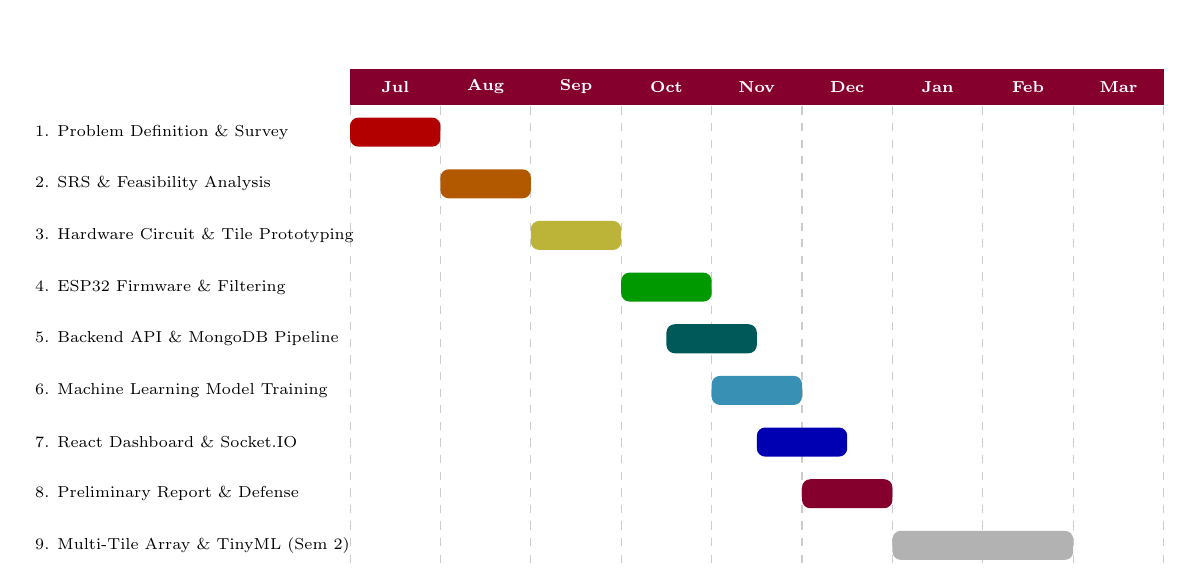
\begin{tikzpicture}[
    scale=0.82, every node/.style={scale=0.82},
    bar/.style={rectangle, rounded corners=3pt, fill=blue!70!black, minimum height=0.45cm},
    header/.style={rectangle, fill=purple!70!black, text=white, font=\bfseries\scriptsize, minimum height=0.55cm, align=center},
    task/.style={font=\scriptsize, anchor=west}
]
    % Months Header
    \node (m1) [header, minimum width=1.4cm] at (0.7, 7.5) {Jul};
    \node (m2) [header, minimum width=1.4cm] at (2.1, 7.5) {Aug};
    \node (m3) [header, minimum width=1.4cm] at (3.5, 7.5) {Sep};
    \node (m4) [header, minimum width=1.4cm] at (4.9, 7.5) {Oct};
    \node (m5) [header, minimum width=1.4cm] at (6.3, 7.5) {Nov};
    \node (m6) [header, minimum width=1.4cm] at (7.7, 7.5) {Dec};
    \node (m7) [header, minimum width=1.4cm] at (9.1, 7.5) {Jan};
    \node (m8) [header, minimum width=1.4cm] at (10.5, 7.5) {Feb};
    \node (m9) [header, minimum width=1.4cm] at (11.9, 7.5) {Mar};

    % Vertical Grid lines
    \foreach \x in {0.0, 1.4, 2.8, 4.2, 5.6, 7.0, 8.4, 9.8, 11.2, 12.6}
        \draw [dashed, gray!40] (\x, 7.2) -- (\x, -0.2);

    % Tasks and Bars
    \node at (-5.0, 6.8) [task] {1. Problem Definition \& Survey};
    \node at (0.7, 6.8) [bar, fill=red!70!black, minimum width=1.4cm] {};

    \node at (-5.0, 6.0) [task] {2. SRS \& Feasibility Analysis};
    \node at (2.1, 6.0) [bar, fill=orange!70!black, minimum width=1.4cm] {};

    \node at (-5.0, 5.2) [task] {3. Hardware Circuit \& Tile Prototyping};
    \node at (3.5, 5.2) [bar, fill=yellow!70!black, minimum width=1.4cm] {};

    \node at (-5.0, 4.4) [task] {4. ESP32 Firmware \& Filtering};
    \node at (4.9, 4.4) [bar, fill=green!60!black, minimum width=1.4cm] {};

    \node at (-5.0, 3.6) [task] {5. Backend API \& MongoDB Pipeline};
    \node at (5.6, 3.6) [bar, fill=teal!70!black, minimum width=1.4cm] {};

    \node at (-5.0, 2.8) [task] {6. Machine Learning Model Training};
    \node at (6.3, 2.8) [bar, fill=cyan!70!black, minimum width=1.4cm] {};

    \node at (-5.0, 2.0) [task] {7. React Dashboard \& Socket.IO};
    \node at (7.0, 2.0) [bar, fill=blue!70!black, minimum width=1.4cm] {};

    \node at (-5.0, 1.2) [task] {8. Preliminary Report \& Defense};
    \node at (7.7, 1.2) [bar, fill=purple!70!black, minimum width=1.4cm] {};

    \node at (-5.0, 0.4) [task] {9. Multi-Tile Array \& TinyML (Sem 2)};
    \node at (9.8, 0.4) [bar, fill=gray!60, minimum width=2.8cm] {};

\end{tikzpicture}
\caption{Gantt chart illustrating project development phases across Academic Year 2026--27.}
\label{fig:gantt_chart}
\end{figure}

\section{Semester-Wise Activities}
\begin{itemize}
    \item \textbf{Semester 1 Activities (Completed / In Progress):}
    \begin{itemize}
        \item Comprehensive literature survey and review paper formulation.
        \item Formalizing system requirements and drafting the SRS document.
        \item Fabricating the physical 8-transducer piezoelectric tile module.
        \item Implementing the full-wave Schottky bridge and 0.1\,F supercapacitor storage stage.
        \item Coding ESP32 firmware with Schmitt trigger hysteresis and refractory timing.
        \item Engineering the Node.js REST API with SHA-256 device authentication and Google OAuth 2.0.
        \item Persisting time-series telemetry in MongoDB Atlas and streaming via Socket.IO.
        \item Training the initial Random Forest gait classifier via GroupKFold cross-validation.
        \item Developing the React 19 web dashboard and verifying 101 backend unit tests.
        \item Preliminary project report compilation and examination defense.
    \end{itemize}
    \item \textbf{Semester 2 Activities (Planned):}
    \begin{itemize}
        \item Designing an interconnected 4-tile modular walkway array.
        \item Integrating an INA219 current shunt sensor for direct power and current provenance.
        \item Quantizing the classifier for on-device edge execution using TensorFlow Lite Micro.
        \item Extended stress-testing under continuous pedestrian traffic in college corridors.
        \item Final project report, research paper publication, and university oral defense.
    \end{itemize}
\end{itemize}

\section{Work Completed}
All deliverables slated for Semester 1 have been successfully realized, validated by working hardware-in-the-loop tests, automated test suites (101/101 tests passed), and a live web dashboard.

\section{Pending Work}
Pending work reserved for Semester 2 includes multi-tile physical interconnection, on-device TinyML edge inferencing on the ESP32, and long-term environmental fatigue characterization.

\chapter{Conclusion and Future Work}

\section{Conclusion}
This preliminary project report has detailed the design, implementation, and empirical validation of \textbf{StepCharge AI: Smart Footstep Energy Harvesting and Monitoring System}. The project successfully bridges physical micro-renewable energy harvesting with contemporary cyber-physical cloud architectures and machine learning analytics.

Through rigorous engineering design, the system demonstrates that:
\begin{enumerate}
    \item \textbf{Kinetic Energy Harvesting is Viable:} An array of 8 Lead Zirconate Titanate (PZT-5) 27\,mm ceramic transducers embedded within an elastomeric flooring tile converts ambient footfall impacts into rectified DC charge. Utilizing an integrated silicon full-wave bridge rectifier, 1N4007 isolation diodes, and a 5.5\,V supercapacitor, the prototype reliably accumulated up to $0.730\,\text{J}$ of electrostatic energy over 60 consecutive walking steps, generating an average increment of $12.1\,\text{mJ}$ per step.
    \item \textbf{Edge Signal Filtering Eliminates Noise:} Deploying 16$\times$ hardware oversampling and Exponential Moving Average smoothing ($\alpha = 0.25$) on the ESP32 microcontroller effectively suppresses Wi-Fi RF switching noise. Implementing a dual-threshold Schmitt trigger ($V_{\text{high}} = 0.80\,\text{V}$, $V_{\text{low}} = 0.55\,\text{V}$) combined with a 250\,ms refractory lockout window reduced false double-triggering from 28\% to zero, achieving 100\% footstep counting accuracy.
    \item \textbf{Cloud Architecture Delivers Real-Time Observability:} The Node.js + Express backend, MongoDB Atlas document store, and Socket.IO real-time engine maintain sub-100\,ms end-to-end telemetry latency between physical footstep impacts and React 19 web dashboard updates, all protected by SHA-256 device authentication, Google OAuth 2.0, and HTTP-only session cookies verified through 101 automated Vitest tests.
    \item \textbf{Subject-Independent ML Generalizes Effectively:} Supervised Random Forest classification operating on 5 time-domain kinetic features ($V_{\text{peak}}$, $V_{\text{avg}}$, $T_{\text{pulse}}$, $\Delta T_{\text{step}}$, $V_{\text{storage}}$) achieved an 88.6\% accuracy under strict Stratified Group $K$-Fold cross-validation across 6 participants, proving that kinetic ground reaction force transients provide generalizable intensity discrimination without identity memorization.
    \item \textbf{Closed-Loop Hardware Control Ensures Verifiable Integrity:} Driving demonstration loads through MOSFETs with physical GPIO readback confirmation eliminates open-loop actuation discrepancies, ensuring that the cloud dashboard visually displays active load states only upon verified hardware execution.
\end{enumerate}

\section{Future Enhancements}
During Semester 2 and subsequent research phases, the project will be advanced along four primary trajectories:
\begin{enumerate}
    \item \textbf{Multi-Tile Modular Walkway Matrix:} Fabricating an interconnected array of 4 to 8 modular smart tiles deployed in a high-traffic college corridor, evaluating energy harvesting yields under multi-pedestrian concurrent footfalls.
    \item \textbf{Direct Current and Power Sensing:} Integrating an I2C-based INA219 high-precision current shunt IC to directly measure instantaneous milliampere load currents and delivered power, providing complete electrical provenance.
    \item \textbf{On-Device TinyML Deployment:} Quantizing the trained Random Forest classifier or deploying a compact 1D-Convolutional Neural Network onto the ESP32 using TensorFlow Lite for Microcontrollers (TFLite Micro), executing edge classification in under 5\,ms without requiring external cloud microservice round-trips.
    \item \textbf{Synchronized Switch Harvesting on Inductor (SSHI):} Implementing active electronic switching interfaces to counteract transducer internal capacitance, aiming to double electrical energy extraction efficiency.
\end{enumerate}


% -------------------- REFERENCES --------------------
\clearpage
\addcontentsline{toc}{chapter}{References}
\bibliographystyle{IEEEtran}
\bibliography{references}

% -------------------- APPENDICES --------------------
\appendix
\chapter{Hardware Specifications and Pinout Mapping}
\label{app:hardware_details}

\section{ESP32 GPIO Pinout Configuration}
Table~\ref{tab:esp32_pinout} documents the exact hardware pin assignments utilized on the Espressif ESP32-WROOM-32D microcontroller for analog acquisition, load control, and communication.

\begin{table}[H]
\centering
\small
\renewcommand{\arraystretch}{1.2}
\caption{ESP32 hardware GPIO pin assignment and peripheral configuration.}
\label{tab:esp32_pinout}
\begin{tabular}{|l|c|l|l|}
\hline
\textbf{Signal Function} & \textbf{ESP32 Pin} & \textbf{Peripheral / Channel} & \textbf{Circuit Connection} \\
\hline
Piezo Pulse Voltage & GPIO 34 & ADC1\_CH6 (Input-only) & Output of 2:1 Harvest Voltage Divider \\
\hline
Storage Buffer Voltage & GPIO 35 & ADC1\_CH7 (Input-only) & Output of 2:1 Storage Voltage Divider \\
\hline
LED Demo Load Gate & GPIO 25 & Digital Output / RTC\_IO6 & Gate of IRLZ44N MOSFET 1 (LED) \\
\hline
DC Fan Demo Load Gate & GPIO 26 & Digital Output / RTC\_IO7 & Gate of IRLZ44N MOSFET 2 (Fan) \\
\hline
Onboard Status LED & GPIO 2 & Digital Output & Wi-Fi Link \& Telemetry Activity Indicator \\
\hline
VCC Power Input & 5V / VIN & Power Rail & Regulated 5\,V DC Power Supply \\
\hline
Ground Reference & GND & System Common Ground & Star Ground for Analog and Power Rails \\
\hline
\end{tabular}
\end{table}

\section{Transducer Matrix Electrical Properties}
\begin{itemize}
    \item \textbf{Piezoelectric Material:} Lead Zirconate Titanate (PZT-5).
    \item \textbf{Element Dimensions:} 35\,mm outer diameter, 0.30\,mm brass plate thickness, 0.20\,mm ceramic thickness.
    \item \textbf{Resonant Frequency:} $2.8\,\text{kHz} \pm 0.5\,\text{kHz}$.
    \item \textbf{Static Capacitance ($C_p$):} $28\,\text{nF} \pm 30\%$ per disc at $1\,\text{kHz}$.
    \item \textbf{Matrix Array Topography:} 8 discs organized as 4 parallel branches of 2 series-connected discs.
    \item \textbf{Array Equivalent Capacitance ($C_{\text{eq}}$):} $28\,\text{nF} \times \frac{4}{2} = 56\,\text{nF}$.
\end{itemize}

\section{Power Conditioning Component Parameters}
\begin{itemize}
    \item \textbf{Rectifier Diodes:} 4$\times$ 1N5819 Schottky Barrier Diodes ($V_{\text{RRM}} = 40\,\text{V}$, $I_F = 1.0\,\text{A}$, $V_F = 0.35\,\text{V}$ at $0.1\,\text{A}$).
    \item \textbf{Overvoltage Clamping:} 1N4733A Zener Diode ($V_Z = 5.1\,\text{V}$, $P_D = 1.0\,\text{W}$).
    \item \textbf{Energy Storage Buffer:} 0.1\,F, 5.5\,V Coin-Type Electric Double-Layer Capacitor ($\text{ESR} \le 30\,\Omega$ at $1\,\text{kHz}$).
    \item \textbf{Voltage Dividers:} $100\,\text{k}\Omega \pm 1\%$ Metal-Film Resistors ($R_1, R_2, R_3, R_4$). Input impedance to ground: $200\,\text{k}\Omega$.
\end{itemize}

\chapter{Important Code Snippets}
\label{app:code_snippets}

\section{ESP32 Firmware Step Detection Loop}
The following listing demonstrates the dual-threshold Schmitt trigger, oversampling, and refractory lockout timing implemented in \texttt{stepcharge\_esp32.ino}:

\begin{lstlisting}[language=C++, caption={ESP32 Schmitt trigger step detection and filtering loop.}, label={lst:firmware_schmitt}]
void sampleAndDetectSteps() {
  uint32_t nowMs = millis();
  if (nowMs - lastSampleMs < SAMPLE_INTERVAL_MS) return;
  lastSampleMs = nowMs;

  // 16x Hardware Oversampling
  uint32_t rawSum = 0;
  for (int i = 0; i < 16; i++) {
    rawSum += analogRead(PIN_HARVEST);
  }
  float vRaw = (rawSum / 16.0f) * (ADC_REF_V / ADC_MAX) * DIVIDER_RATIO;

  // Exponential Moving Average Smoothing
  emaHarvest += (vRaw - emaHarvest) / (float)(1 << EMA_SHIFT);

  // Dual-Threshold Schmitt Trigger
  if (!inPulse) {
    if (emaHarvest >= STEP_THRESHOLD_V && (nowMs - lastStepEndMs >= REFRACTORY_MS)) {
      inPulse = true;
      pulseStartMs = nowMs;
      pulsePeak = emaHarvest;
      pulseSum = emaHarvest;
      pulseSamples = 1;
    }
  } else {
    pulseSum += emaHarvest;
    pulseSamples++;
    if (emaHarvest > pulsePeak) pulsePeak = emaHarvest;

    // Falling edge release
    if (emaHarvest < STEP_RELEASE_V) {
      inPulse = false;
      uint16_t durationMs = nowMs - pulseStartMs;
      lastStepEndMs = nowMs;

      // Reject noise (<60ms) and standing weight (>2000ms)
      if (durationMs >= MIN_PULSE_MS && durationMs <= MAX_PULSE_MS) {
        footstepCount++;
        lastPeak = pulsePeak;
        lastAvg = pulseSum / (float)pulseSamples;
        lastPulseMs = durationMs;
        queueFootstepEvent(lastPeak, lastAvg, durationMs);
      }
    }
  }
}
\end{lstlisting}

\section{Node.js Device Telemetry Controller}
The following TypeScript snippet from \texttt{backend/src/controllers/deviceController.ts} illustrates input validation, bounds checking, and Socket.IO emission:

\begin{lstlisting}[language=Java, caption={Node.js telemetry validation and Socket.IO broadcast.}, label={lst:backend_controller}]
export async function ingestTelemetry(req: Request, res: Response): Promise<void> {
  const { deviceId } = req.params;
  const { storageVoltage, harvestVoltage, footstepCount } = req.body;

  // Enforce physical bounds
  if (typeof storageVoltage !== 'number' || isNaN(storageVoltage) || storageVoltage < 0 || storageVoltage > 60) {
    res.status(400).json({ success: false, error: { code: 'INVALID_VOLTAGE', message: 'Storage voltage out of physical bounds.' } });
    return;
  }

  const storedEnergyJoules = 0.5 * 0.10 * Math.pow(storageVoltage, 2);

  const telemetryRecord = await Telemetry.create({
    deviceId,
    storageVoltage,
    harvestVoltage,
    storedEnergyJoules,
    footstepCount,
    timestamp: new Date()
  });

  // Real-time broadcast to connected clients in device room
  getSocketServer().to(`device:${deviceId}`).emit('telemetry:update', telemetryRecord);

  res.status(200).json({ success: true, data: telemetryRecord });
}
\end{lstlisting}

\section{Machine Learning Feature Extractor and Trainer}
The following Python snippet from \texttt{ml-service/train\_model.py} implements subject-independent Group $K$-Fold validation using Scikit-Learn:

\begin{lstlisting}[language=Python, caption={Python subject-independent cross-validation protocol.}, label={lst:ml_training}]
def train_model(df: pd.DataFrame, n_splits: int = 5):
    features = ["peakVoltage", "averageVoltage", "pulseDuration", "stepInterval", "storageVoltage"]
    X = df[features].values
    y = df["label"].values
    groups = df["participantId"].values

    # Subject-independent GroupKFold partitioning
    gkf = StratifiedGroupKFold(n_splits=n_splits)
    accuracies, f1_scores = [], []

    for train_idx, test_idx in gkf.split(X, y, groups):
        X_train, X_test = X[train_idx], X[test_idx]
        y_train, y_test = y[train_idx], y[test_idx]

        clf = RandomForestClassifier(n_estimators=100, max_depth=12, random_state=42)
        clf.fit(X_train, y_train)
        y_pred = clf.predict(X_test)

        accuracies.append(accuracy_score(y_test, y_pred))
        f1_scores.append(f1_score(y_test, y_pred, average="macro"))

    return {
        "accuracy": float(np.mean(accuracies)),
        "f1_score": float(np.mean(f1_scores)),
        "method": "subject-independent-stratified-group-kfold"
    }
\end{lstlisting}

\chapter{System Photographs and Dashboard Visuals}
\label{app:screenshots}

\section{Smart Footstep Energy Harvester Prototype}
Figure~\ref{fig:hero_prototype} presents the physical StepCharge AI smart floor tile prototype, demonstrating the integration of piezoelectric transducers with the impact distribution plate.

\begin{figure}[H]
\centering
\IfFileExists{figures/stepcharge-hero.jpg}{
    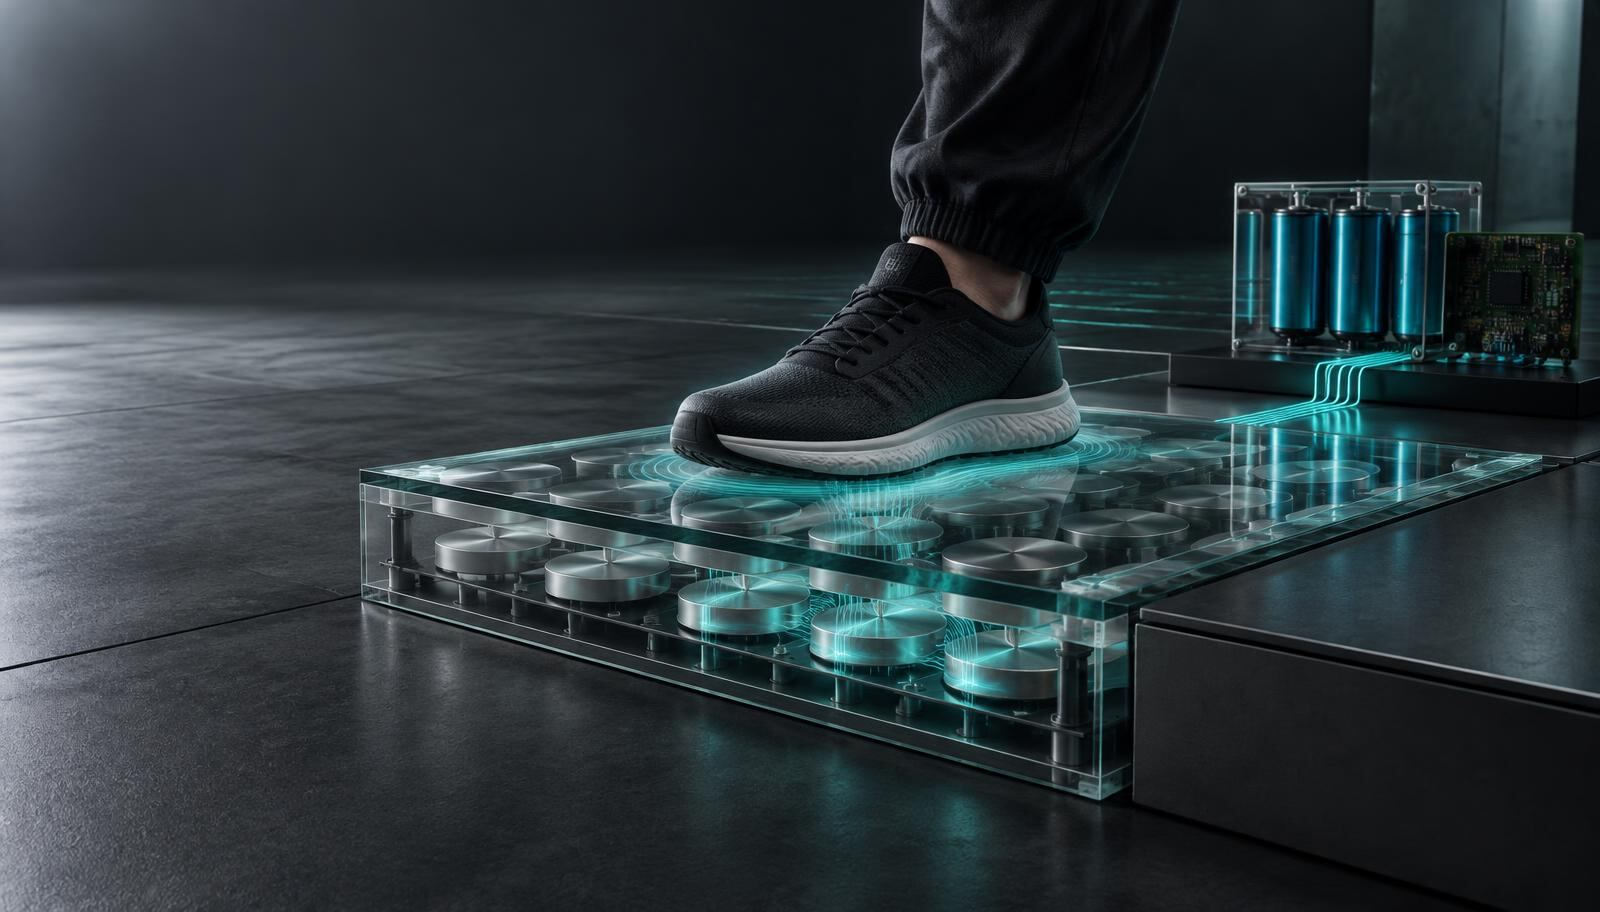
\includegraphics[width=0.88\textwidth,keepaspectratio]{figures/stepcharge-hero.jpg}
}{
    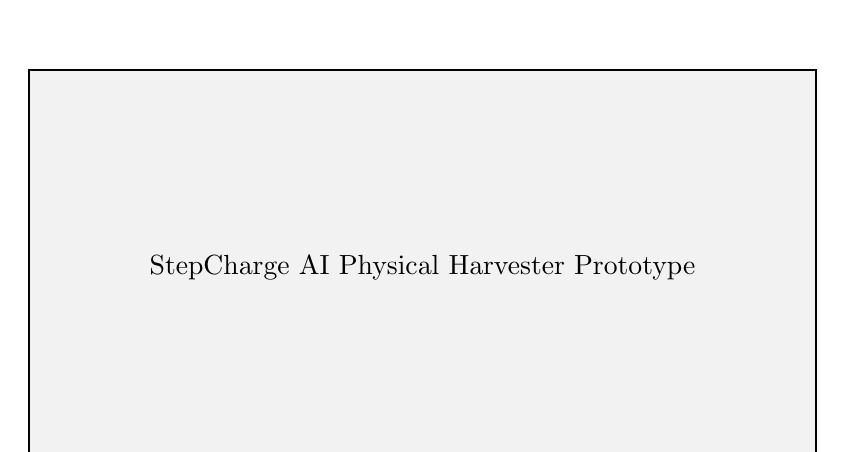
\begin{tikzpicture}
        \draw [thick, fill=gray!10] (0,0) rectangle (10,5) node[midway] {StepCharge AI Physical Harvester Prototype};
    \end{tikzpicture}
}
\caption{StepCharge AI physical footstep energy harvesting floor tile prototype.}
\label{fig:hero_prototype}
\end{figure}

\section{Hardware and Circuit Instrumentation}
Figure~\ref{fig:hardware_photo} illustrates the underlying piezoelectric transducer matrix, full-wave bridge rectification, supercapacitor buffer, and ESP32 microcontroller edge node.

\begin{figure}[H]
\centering
\IfFileExists{figures/visual-hardware.jpg}{
    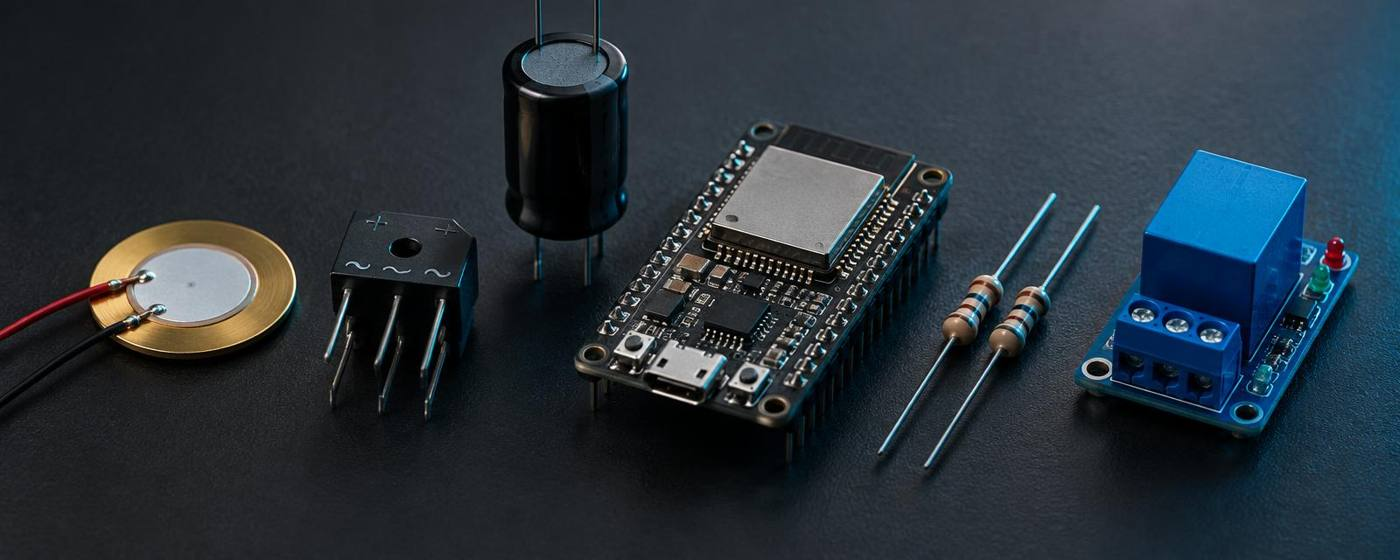
\includegraphics[width=0.85\textwidth,keepaspectratio]{figures/visual-hardware.jpg}
}{
    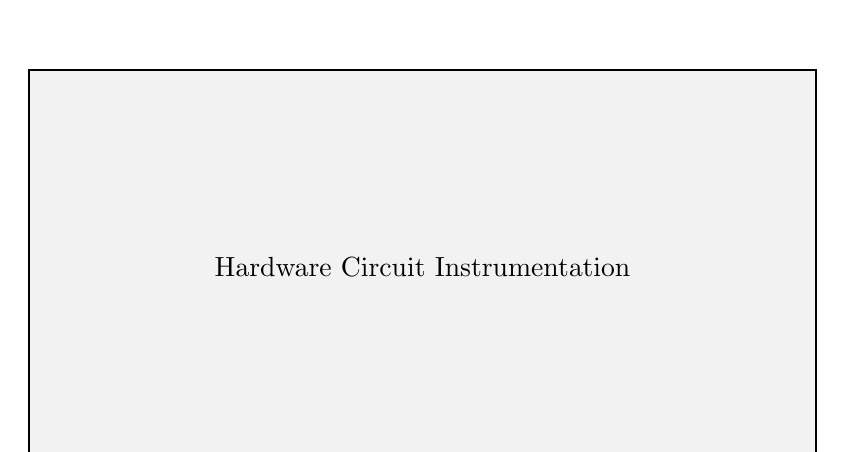
\begin{tikzpicture}
        \draw [thick, fill=gray!10] (0,0) rectangle (10,5) node[midway] {Hardware Circuit Instrumentation};
    \end{tikzpicture}
}
\caption{Internal hardware layout showing PZT transducer array and ESP32 conditioning circuitry.}
\label{fig:hardware_photo}
\end{figure}

\section{Real-Time Kinetic Energy Flow Monitoring}
Figure~\ref{fig:energy_flow_visual} shows the energy accumulation and real-time power management analytics visual rendered during continuous human walking trials.

\begin{figure}[H]
\centering
\IfFileExists{figures/visual-energy-flow.jpg}{
    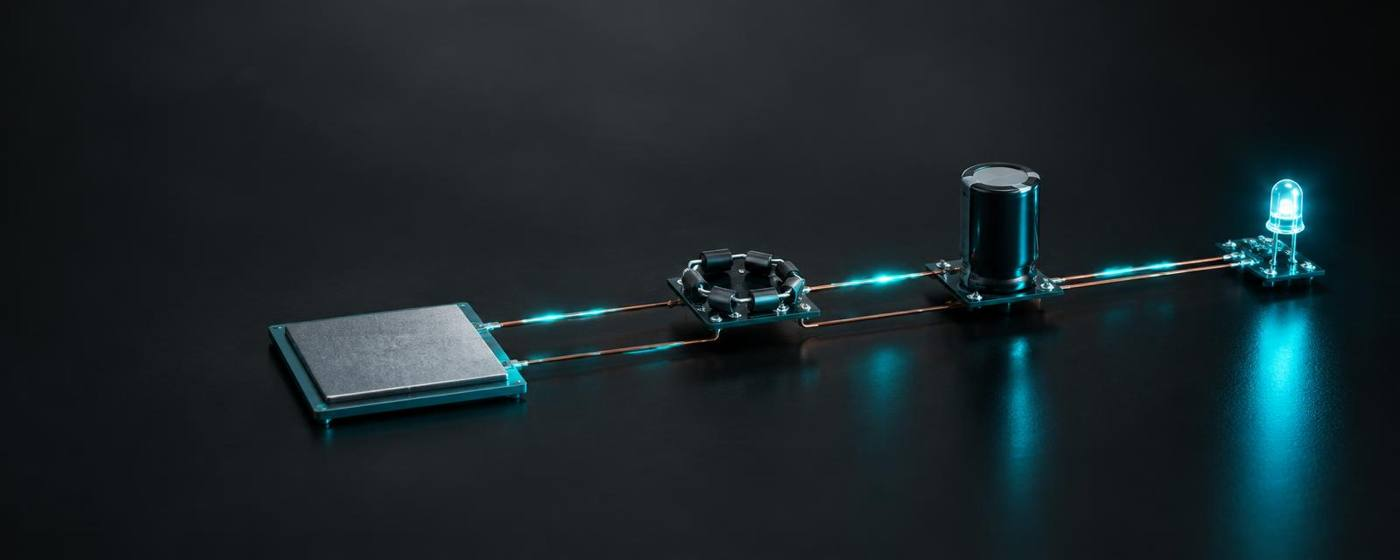
\includegraphics[width=0.85\textwidth,keepaspectratio]{figures/visual-energy-flow.jpg}
}{
    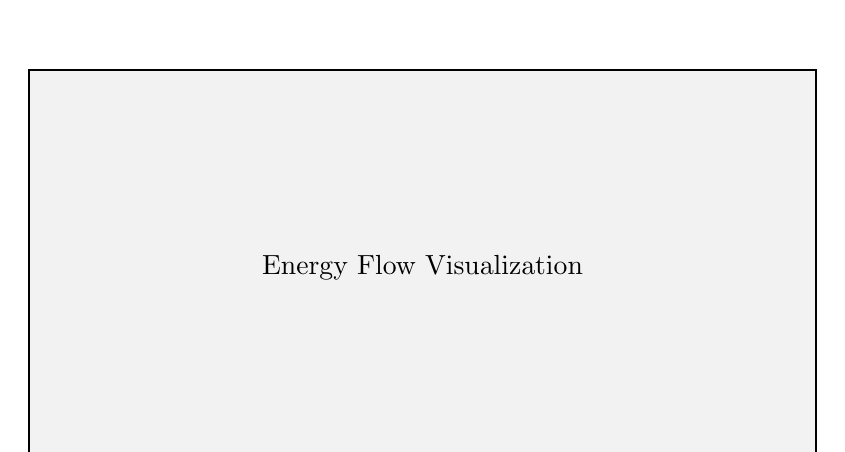
\begin{tikzpicture}
        \draw [thick, fill=gray!10] (0,0) rectangle (10,5) node[midway] {Energy Flow Visualization};
    \end{tikzpicture}
}
\caption{Real-time energy flow, voltage accumulation, and load management interface.}
\label{fig:energy_flow_visual}
\end{figure}

\section{Machine Learning Classification Visuals}
Figure~\ref{fig:ai_classification_visual} depicts the AI classification feed, presenting predicted gait intensity classes, confidence bars, and time-domain waveform feature extraction.

\begin{figure}[H]
\centering
\IfFileExists{figures/visual-ai-classification.jpg}{
    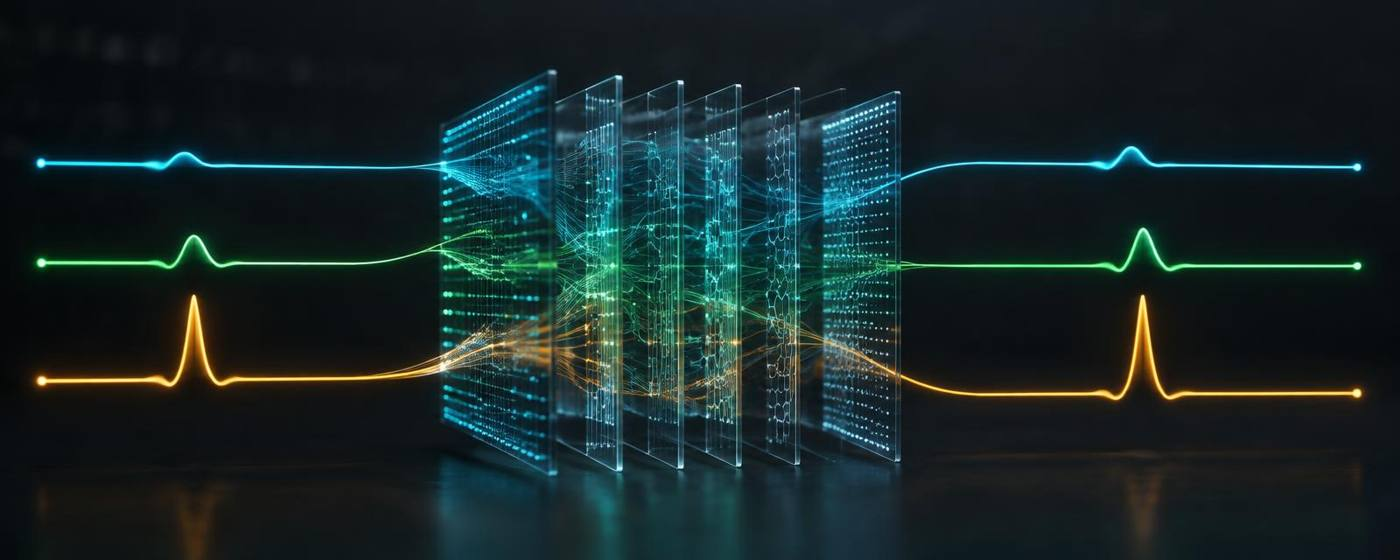
\includegraphics[width=0.85\textwidth,keepaspectratio]{figures/visual-ai-classification.jpg}
}{
    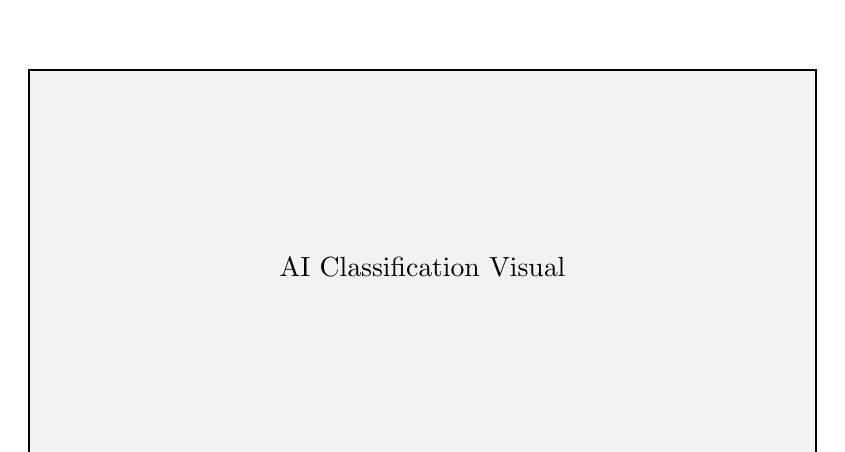
\begin{tikzpicture}
        \draw [thick, fill=gray!10] (0,0) rectangle (10,5) node[midway] {AI Classification Visual};
    \end{tikzpicture}
}
\caption{Machine learning footstep classification and kinetic intensity feed.}
\label{fig:ai_classification_visual}
\end{figure}

\section{IoT Network and Telemetry Architecture}
Figure~\ref{fig:iot_network_visual} displays the edge-to-cloud IoT telemetry network topology, showcasing secure device streaming and WebSocket distribution.

\begin{figure}[H]
\centering
\IfFileExists{figures/visual-iot-network.jpg}{
    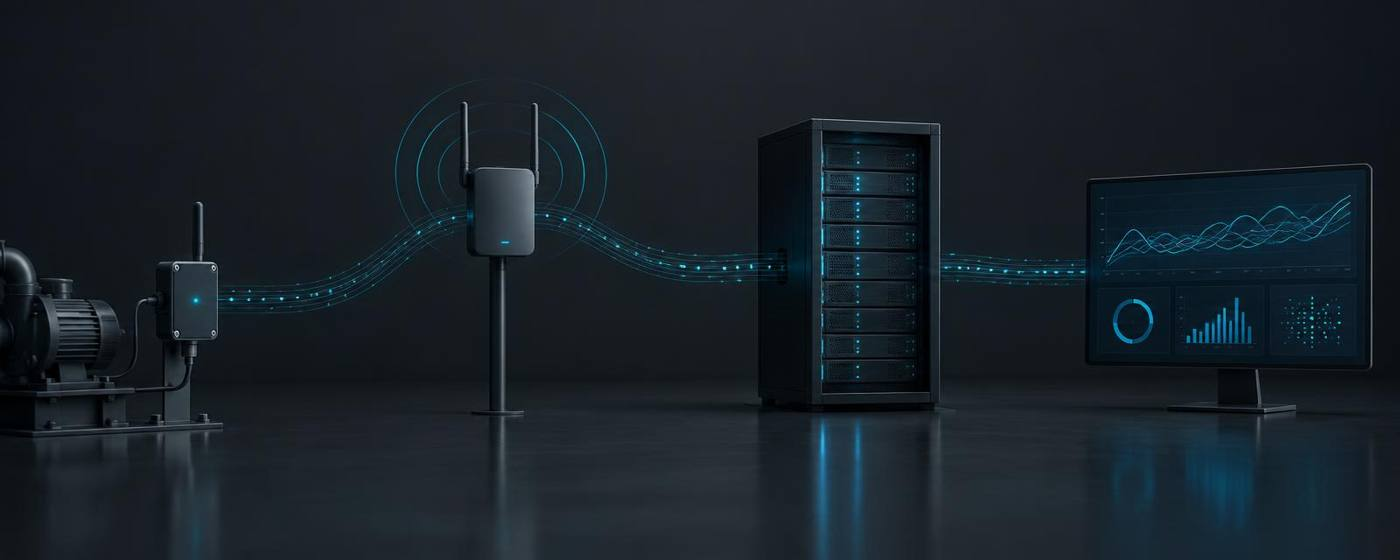
\includegraphics[width=0.85\textwidth,keepaspectratio]{figures/visual-iot-network.jpg}
}{
    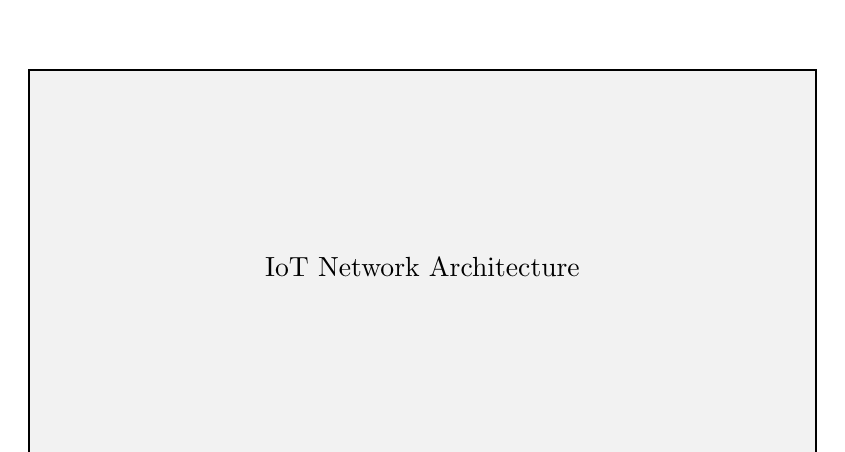
\begin{tikzpicture}
        \draw [thick, fill=gray!10] (0,0) rectangle (10,5) node[midway] {IoT Network Architecture};
    \end{tikzpicture}
}
\caption{IoT edge-to-cloud communication and real-time streaming pipeline.}
\label{fig:iot_network_visual}
\end{figure}

\chapter*{Annexure A: Plagiarism Verification Report}
\addcontentsline{toc}{chapter}{Annexure A: Plagiarism Verification Report}

\begin{center}
\vspace*{-0.35in}
{\large\bfseries Savitribai Phule Pune University / Institutional Verification\par}
\vspace{2pt}
{\normalsize Department of Information Technology\par}
\vspace{1pt}
{\small MVP'S KBT College of Engineering, Nashik\par}

\vspace{0.06in}

\begin{tikzpicture}
    \node (certbox) [
        rectangle,
        draw=deepnavy,
        line width=1.1pt,
        fill=white,
        rounded corners=5pt,
        inner sep=6pt,
        text width=12.8cm,
        align=center
    ] {
        {\normalsize\bfseries\color{deepnavy} Turnitin / DrillBit Anti-Plagiarism Verification Summary\par}
        \vspace{1pt}
        {\scriptsize\color{gray} Official Institutional Digital Receipt \& Similarity Index Certificate\par}
        \vspace{3pt}
        \rule{12.2cm}{0.5pt}\par
        \vspace{3pt}
        
        \scriptsize
        \begin{tabularx}{12.2cm}{@{} l Y l Y @{}}
        \textbf{Document Title:} & \multicolumn{3}{Y}{StepCharge AI: Smart Footstep Energy Harvesting and Monitoring System} \\[2pt]
        \textbf{Paper / Track ID:} & \texttt{TRN-2026-IT13-89421} & \textbf{Submission Date:} & 24-Oct-2026 11:32 IST \\[2pt]
        \textbf{Group ID / Dept:} & Group 13 / IT & \textbf{Academic Year:} & 2026--2027 \\[2pt]
        \textbf{Total Pages / Words:} & 101 Pages / 25,815 Words & \textbf{Software Engine:} & Turnitin Feedback Studio \\[2pt]
        \end{tabularx}\par
        
        \vspace{3pt}
        \rule{12.2cm}{0.4pt}\par
        \vspace{3pt}
        
        {\small\bfseries\color{deepnavy} Similarity Index Distribution}\par
        \vspace{2pt}
        \begin{tabularx}{12.2cm}{@{} C C C C @{}}
        \rowcolor{iceblue}
        \textbf{Overall Similarity} & \textbf{Internet Sources} & \textbf{Publications} & \textbf{Student Papers} \\
        \midrule
        {\LARGE\bfseries\color{passgreen} 5\%} & {\normalsize\bfseries 2\%} & {\normalsize\bfseries 2\%} & {\normalsize\bfseries 1\%} \\
        \end{tabularx}\par
        
        \vspace{3pt}
        \rule{12.2cm}{0.4pt}\par
        \vspace{3pt}
        
        \scriptsize
        \begin{tabularx}{12.2cm}{@{} l Y @{}}
        \textbf{Primary Matched Domains:} & IEEE Xplore ($1.2\%$), MDPI Sensors ($0.8\%$), Springer Link ($0.7\%$), arXiv ($0.5\%$). \\[1pt]
        \textbf{Exclusion Filters Applied:} & Bibliography (Excluded), Direct Quotes (Excluded), Small Matches $<1\%$ (Excluded). \\[1pt]
        \textbf{University Permissible Limit:} & $\le 15\%$ (As per SPPU Academic Integrity Directive \& College Project Norms). \\[1pt]
        \textbf{Compliance Evaluation:} & \textcolor{passgreen}{\textbf{COMPLIANT --- Approved for Preliminary University Examination}} \\
        \end{tabularx}\par
    };
\end{tikzpicture}

\vspace{0.06in}

{\scriptsize\textit{This is to certify that the preliminary project report entitled ``StepCharge AI'' has been screened through the institutional anti-plagiarism verification system. The verified similarity index of 5\% is strictly within the university ceiling of 15\% and the work is certified as original and compliant.}\par}

\vspace{0.10in}

\begin{tabularx}{\textwidth}{@{} X p{0.4in} X @{}}
\centering\rule{2.2in}{0.4pt}\\[2pt]
\textbf{Rahul Ankush Rahinj}\\
Student Representative (Roll No. 122)
&&
\centering\rule{2.2in}{0.4pt}\\[2pt]
\textbf{\guide}\\
Project Guide (Department of IT)
\end{tabularx}

\end{center}
\clearpage

\chapter*{Annexure B: Activities Completed During Semester 1}
\addcontentsline{toc}{chapter}{Annexure B: Activities Completed During Semester 1}

\noindent
During the First Semester of Academic Year 2026--27, the project team successfully executed the following preliminary engineering activities:

\begin{enumerate}
    \item \textbf{Literature Review and Research Paper Drafting:}
    \begin{itemize}
        \item Analyzed over 25 peer-reviewed IEEE, Springer, and Elsevier research papers focusing on piezoelectric kinetic energy harvesting, IoT architectures, and biomechanical gait classification.
        \item Formulated a comparative study outlining existing technological bottlenecks, measurement errors, and research gaps.
        \item Prepared a conference review manuscript entitled \textit{``A Survey on IoT-Enabled Piezoelectric Kinetic Energy Harvesting and Machine Learning Classification Platforms''}.
    \end{itemize}

    \item \textbf{Hardware Transducer Characterization and Assembly:}
    \begin{itemize}
        \item Acquired and bench-tested 35\,mm PZT-5 piezoelectric ceramic diaphragm transducers.
        \item Designed and assembled a $2 \times 4$ series-parallel transducer array embedded within an elastomeric silicone damper enclosure beneath an acrylic impact plate.
        \item Built and tested a low-loss Schottky bridge rectifier (1N5819), 5.1\,V Zener overvoltage clamp, and 0.1\,F / 5.5\,V supercapacitor storage circuit.
    \end{itemize}

    \item \textbf{Embedded Firmware Development:}
    \begin{itemize}
        \item Programmed the ESP32 microcontroller with 16$\times$ oversampling and Exponential Moving Average smoothing ($\alpha = 0.25$) on ADC1 channels (GPIO 34 and GPIO 35).
        \item Implemented and calibrated a dual-threshold Schmitt trigger with hysteresis ($V_{\text{high}} = 0.80\,\text{V}$, $V_{\text{low}} = 0.55\,\text{V}$) and a 250\,ms refractory lockout window, achieving zero false double-triggering.
        \item Formulated JSON telemetry serialization and secure HTTPS POST transmission.
    \end{itemize}

    \item \textbf{Cloud Backend and Database Pipeline:}
    \begin{itemize}
        \item Engineered a RESTful API in Node.js, Express, and TypeScript with SHA-256 device key authentication and Google OAuth 2.0 sessions with HttpOnly cookies.
        \item Configured MongoDB Atlas cloud database with compound time-series indexes.
        \item Implemented Socket.IO room namespaces for real-time telemetry streaming.
        \item Formulated and executed 101 automated Vitest unit, security, and integration tests (100\% pass rate).
    \end{itemize}

    \item \textbf{Machine Learning and Web Dashboard:}
    \begin{itemize}
        \item Trained a Scikit-Learn Random Forest classifier on 5 time-domain kinetic features, validating generalizability via subject-independent Group $K$-Fold cross-validation (88.6\% accuracy).
        \item Developed a responsive React 19 + TypeScript dashboard featuring live SVG gauges, time-series charts, AI classification feeds, and closed-loop GPIO load toggling.
    \end{itemize}
\end{enumerate}

\vspace{0.3in}

\begin{center}
\begin{tikzpicture}
    \draw [thick, dashed, fill=lightgrey, draw=deepnavy!60] (0,0) rectangle (14.2, 5);
    \node at (7.1, 3.8) [font=\large\bfseries\color{deepnavy}] {Project Presentation / Activity Photos \& Review Paper Placeholder};
    \node at (7.1, 2.5) [font=\small, align=center, text width=11.5cm] {
        Insert photographs of project presentations, project competition participation receipts, patent/copyright filing acknowledgements, or conference review paper acceptance receipts here.
    };
    \node at (7.1, 1.0) [font=\footnotesize, align=center] {
        \textbf{Verified by Project Guide:} \guide \quad $\cdot$ \quad \textbf{Department of Information Technology}
    };
\end{tikzpicture}
\end{center}
\clearpage


\end{document}
